%% 
%% Copyright 2019-2021 Elsevier Ltd
%% 
%% This file is part of the 'CAS Bundle'.
%% --------------------------------------
%% 
%% It may be distributed under the conditions of the LaTeX Project Public
%% License, either version 1.2 of this license or (at your option) any
%% later version.  The latest version of this license is in
%%    http://www.latex-project.org/lppl.txt
%% and version 1.2 or later is part of all distributions of LaTeX
%% version 1999/12/01 or later.
%% 
%% The list of all files belonging to the 'CAS Bundle' is
%% given in the file `manifest.txt'.
%% 
%% Template article for cas-sc documentclass for 
%% single column output.

\documentclass[a4paper,fleqn]{cas-sc}

% If the frontmatter runs over more than one page
% use the longmktitle option.

%\documentclass[a4paper,fleqn,longmktitle]{cas-sc}

%\usepackage[numbers]{natbib}
%\usepackage[authoryear]{natbib}
\usepackage[authoryear,longnamesfirst]{natbib}

%%%Author macros
\def\tsc#1{\csdef{#1}{\textsc{\lowercase{#1}}\xspace}}
\tsc{WGM}
\tsc{QE}
%%%

% Uncomment and use as if needed
%\newtheorem{theorem}{Theorem}
%\newtheorem{lemma}[theorem]{Lemma}
%\newdefinition{rmk}{Remark}
%\newproof{pf}{Proof}
%\newproof{pot}{Proof of Theorem \ref{thm}}
% 加入宏包
\usepackage{graphicx}
\usepackage{subcaption}
\usepackage{lscape}
\usepackage{longtable}
\usepackage{booktabs}

\begin{document}
\let\WriteBookmarks\relax
\def\floatpagepagefraction{1}
\def\textpagefraction{.001}

% Short title
% \shorttitle{<short title of the paper for running head>}   
\shorttitle{short title of the paper for running head}    

% Short author
% \shortauthors{<short author list for running head>} 
\shortauthors{short author list for running head}  

% Main title of the paper
\title [mode = title]{Evaluation on the Necessity of Sentinel-1 TOPS Enhanced Spectral Diversity for InSAR} 

% Title footnote mark
% eg: \tnotemark[1]
% \tnotemark[<tnote number>]
\tnotemark[tnote number] 

% 文献引用
% Title footnote 1.
% eg: \tnotetext[1]{Title footnote text}
% \tnotetext[<tnote number>]{<tnote text>} 

% First author
%
% Options: Use if required
% eg: \author[1,3]{Author Name}[type=editor,
%       style=chinese,
%       auid=000,
%       bioid=1,
%       prefix=Sir,
%       orcid=0000-0000-0000-0000,
%       facebook=<facebook id>,
%       twitter=<twitter id>,
%       linkedin=<linkedin id>,
%       gplus=<gplus id>]

\author[1]{Mengwei Li}

% Corresponding author indication
% \cormark[<corr mark no>]

% Footnote of the first author
% \fnmark[<footnote mark no>]

% Email id of the first author
% \ead{<email address>}
\ead{limengwei@mail.nwpu.edu.cn}

% URL of the first author
% \ead[url]{<URL>}

% Credit authorship
% eg: \credit{Conceptualization of this study, Methodology, Software}
% \credit{<Credit authorship details>}

% Address/affiliation
\affiliation[1]{organization={School of Electronics and Information},
            addressline={Northwestern Polytechnical University}, 
            city={Xi'an},
%          citysep={}, % Uncomment if no comma needed between city and postcode
            postcode={710129}, 
            state={Shaanxi},
            country={China}}

\author[1]{Yuxiao Qin}
\cormark[1]

% Footnote of the second author
% \fnmark[2]

% Email id of the second author
\ead{yuxiao.qin@nwpu.edu.cn}

% URL of the second author
% \ead[url]{}

% Credit authorship
% \credit{}

% Address/affiliation
% \affiliation[<aff no>]{organization={},
%             addressline={}, 
%             city={},
% %          citysep={}, % Uncomment if no comma needed between city and postcode
%             postcode={}, 
%             state={},
%             country={}}

% Corresponding author text
\cortext[1]{Corresponding author}

% Footnote text
\fntext[1]{}

% For a title note without a number/mark
%\nonumnote{}

% Here goes the abstract
\begin{abstract}
Since Sentinel-1 (S-1) was launched in 2014, it has become the most influential SAR satellite in the field of earth observation with its open source policy and rich database. Among them, the existence of the special ‘phase slope’ of the TOPS mode of S-1 default imaging leads to the coregistration of this mode must meet the 0.001 pixel accuracy. Based on this, the use of enhanced spectral diversity (ESD) method after geometrical coregistration has become a recognized necessary step in the conventional coregistration of S-1 TOPS data. However, in recent years, ESA official reports have shown that the 3D RMS of precise orbit data has been better than 1.5 cm, and the corresponding theoretical coregistration accuracy is 0.0015 pixel, so there is no need for ESD secondary resampling to reduce the computational overhead. Whether this inference is true or not needs to be quantitatively verified. Based on the above background, this paper studies the necessity of S-1 TOPS ESD coregistration based on ESA SNAP Sentinel-1 platform for precision orbit data released by ESA. The experimental results show that the accuracy of geometrical coregistration depends on the difference in the accuracy of the repeat orbit. The current precision orbit data released by the ESA has not had a significant impact on the accuracy of geometrical coregistration. At the same time, it is found that the error of geometrical coregistration mainly comes from the orbit error of the master image when registering multiple images of the repeat orbit. When the master image has no orbit error, the standard deviation of the coregistration error caused by the relative orbit error of the slave images relative to the master image is only 0.002 pixel. Experiments show that the difference of ESD offset estimated by different bursts of the same track data is mostly more than 0.001 pixel, but in theory, the ESD offset of different bursts of the same track should be a constant value. Therefore, it is speculated that the coregistration error of 0.002 pixel may mainly come from the atmosphere, not the orbit error. The conclusion shows that if the constant value is used for correction of different bursts in the same orbit, it is possible to mistake the atmospheric error as the coregistration error correction. Based on the above content, this paper gives corresponding suggestions. For time series experiments, the influence of orbit error on phase is usually reduced with time series regression analysis. In the secondary coregistration process, the orbit error of the master image can be corrected by calculating the mean value of multiple interferograms, and the use of ESD may introduce additional errors. For a single image experiment, the orbit error of the master image cannot be effectively estimated. When ESD must be used, this paper proposes a coregistration method based on phase without resampling, which can save 40\% of the calculation time.
\end{abstract}

% Use if graphical abstract is present
%\begin{graphicalabstract}
%\includegraphics{}
%\end{graphicalabstract}

% Research highlights
\begin{highlights}
\item 
\item 
\item 
\end{highlights}

% Keywords
% Each keyword is seperated by \sep
\begin{keywords}
Enhanced spectral diversity \sep Sentinel-1 \sep Terrain observation by progressive scans \sep Coregistration
\end{keywords}

\maketitle

% Main text
\section{Introduction}\label{Introduction}

The Sentinel-1(S-1) satellite is an earth observation satellite of the ESA Copernicus program. It carries a C-band synthetic aperture radar imaging sensor and has a scanning imaging mode to achieve wide-area coverage. S-1’s new imaging mode, Terrain Observation by Progressive Scans (TOPS) mode, better realizes the routine operation of wide-area surface observation. However, the Doppler frequency change will cause the phase slope, especially the influence on the azimuth direction can not be eliminated \cite{A_Study_of_Sentinel-1_TOPS_Mode_Co-registration}. Therefore, this mode requires higher coregistration accuracy for subsequent processing and application. The conventional initial coregistration method may not meet the corresponding accuracy requirements, and the enhanced spectral diversity (ESD) method must be used for fine coregistration to obtain the correct interferogram. \par

The geometrical coregistration is one of the most widely-applied coregistration methods. The essence of this method is to obtain the global shift between the master and slave images based on the zero-Doppler geometry of Synthetic Aperture Radar (SAR) images, and its accuracy is mainly affected by the satellite orbit. After using precise orbit products, the orbit accuracy of S-1 satellite is controlled within 5cm \cite{Interferometric_Processing_of_Sentinel-1_TOPS_Data, A_Study_of_Sentinel-1_TOPS_Mode_Co-registration}. In particular, after the orbit adjustment in 2020, it is found in the report of ESA COPERNICUS POD REGULAR SERVICE REVIEW that the orbit accuracy evaluation results of S-1A satellite are gradually improved. Mean of daily RMS less than 1.5cm \cite{copernicus_review_2020.10-2020.12, copernicus_review_2021.01-2021.12, copernicus_review_2022.01-2022.12}. The control of satellite orbit is beneficial to improve the accuracy of the geometrical coregistration. \par

The essence of ESD is to use the phase difference of the overlapping areas between bursts to obtain the shift required for coregistration. The larger the satellite steering angle is, the more sensitive it is to the coregistration error and the higher the coregistration accuracy is \cite{TOPS_Interferometry_With_TerraSAR-X}. However, there is a certain risk to rely solely on the phase difference, which may be affected by large ground displacement, nonstationary miscoregistration and so on. Eventually, the reliability and validity of the valuation are low. At the same time, the mismatch accuracy of ESD is affected by the coherence between SAR images, especially the time decorrelation. The low coherence interferograms can lead to inaccurate estimation of the azimuth miscoregistration. If the orbit accuracy is high enough, only the geometrical coregistration can meet the demand, then ESD will not be necessary for SAR Interferometry (InSAR) and multi-temporal InSAR (MT-InSAR). \par

In historical studies, the ESD method has been applied to TerraSAR-X and S-1 data processing, and has shown good coregistration results \cite{Interferometry_with_TOPS:_coregistration_and_azimuth_shifts, Interferometric_Processing_of_Sentinel-1_TOPS_Data}. The network-based ESD method estimates mismatches by overlapping interferograms of short-term baselines, reducing the negative impact of temporal coherence \cite{A_Network-Based_Enhanced_Spectral_Diversity_Approach_for_TOPS_Time-Series_Analysis}. At present, ESD has become a very critical step in TOPS mode data processing with its extremely high coregistration accuracy. \par

In view of the above situation and thinking, this paper uses the ESD method to calculate the residual error of geometrical coregistration with the assistance of the precision orbit data released by the ESA, judges and evaluates the necessity of the ESD method with the assistance of higher precision orbit data, and studies the method of improving the coregistration efficiency. In the part of ‘Theory’, the requirements of S-1 TOPS coregistration are introduced, and the relationship between geometrical coregistration, ESD and precise orbit data is described. In the part of ‘Method’, the master image correction method and the coregistration method based on phase without resampling are proposed, which greatly improves the coregistration efficiency. In the part of ‘Experiment’, through the interference comparison experiment of a large number of data, the influence of precise orbit data on the residual error of geometrical coregistration is analyzed, and the reliability of ESD results is judged. Finally, the change and magnitude of residual error are explained, and the necessity of ESD is suggested. \par


\section{Theory}\label{Theory}

\subsection{S-1 TOPS Coregistration Accuracy Requirement}
The S-1 satellite mission is to provide an all-weather, day-and-night supply of imagery of Earth’s surface. Among them, TOPS pattern for S-1 Interferometric Wide swath (IW) mode is the main acquisition mode on land, which meets the needs of large-scale land system monitoring, and is also the target mode of this paper. The TOPS pattern for S-1 IW mode is shown in \ref{fig_1}. The corresponding parameters are shown in \ref{table_1}. It can be seen from \ref{fig_1} that in TOPS mode, the satellite has the characteristics of squint imaging, that is, there is squint angle. The greater the change of the squint angle in the azimuth direction, the more obvious the interference phase difference will be generated, which is also called the phase slope. Fundamentally, the sweeping of antenna introduces a quadratic Doppler frequency in azimuth that exceeds the Pulse Repetition Frequency (PRF). Especially at the burst edge, the phase ramp phenomenon is the most obvious, which will lead to interferogram distortion. Therefore, this pattern requires higher coregistration accuracy \cite{Interferometry_with_TOPS:_coregistration_and_azimuth_shifts}. \par

\begin{figure}
	\centering 
	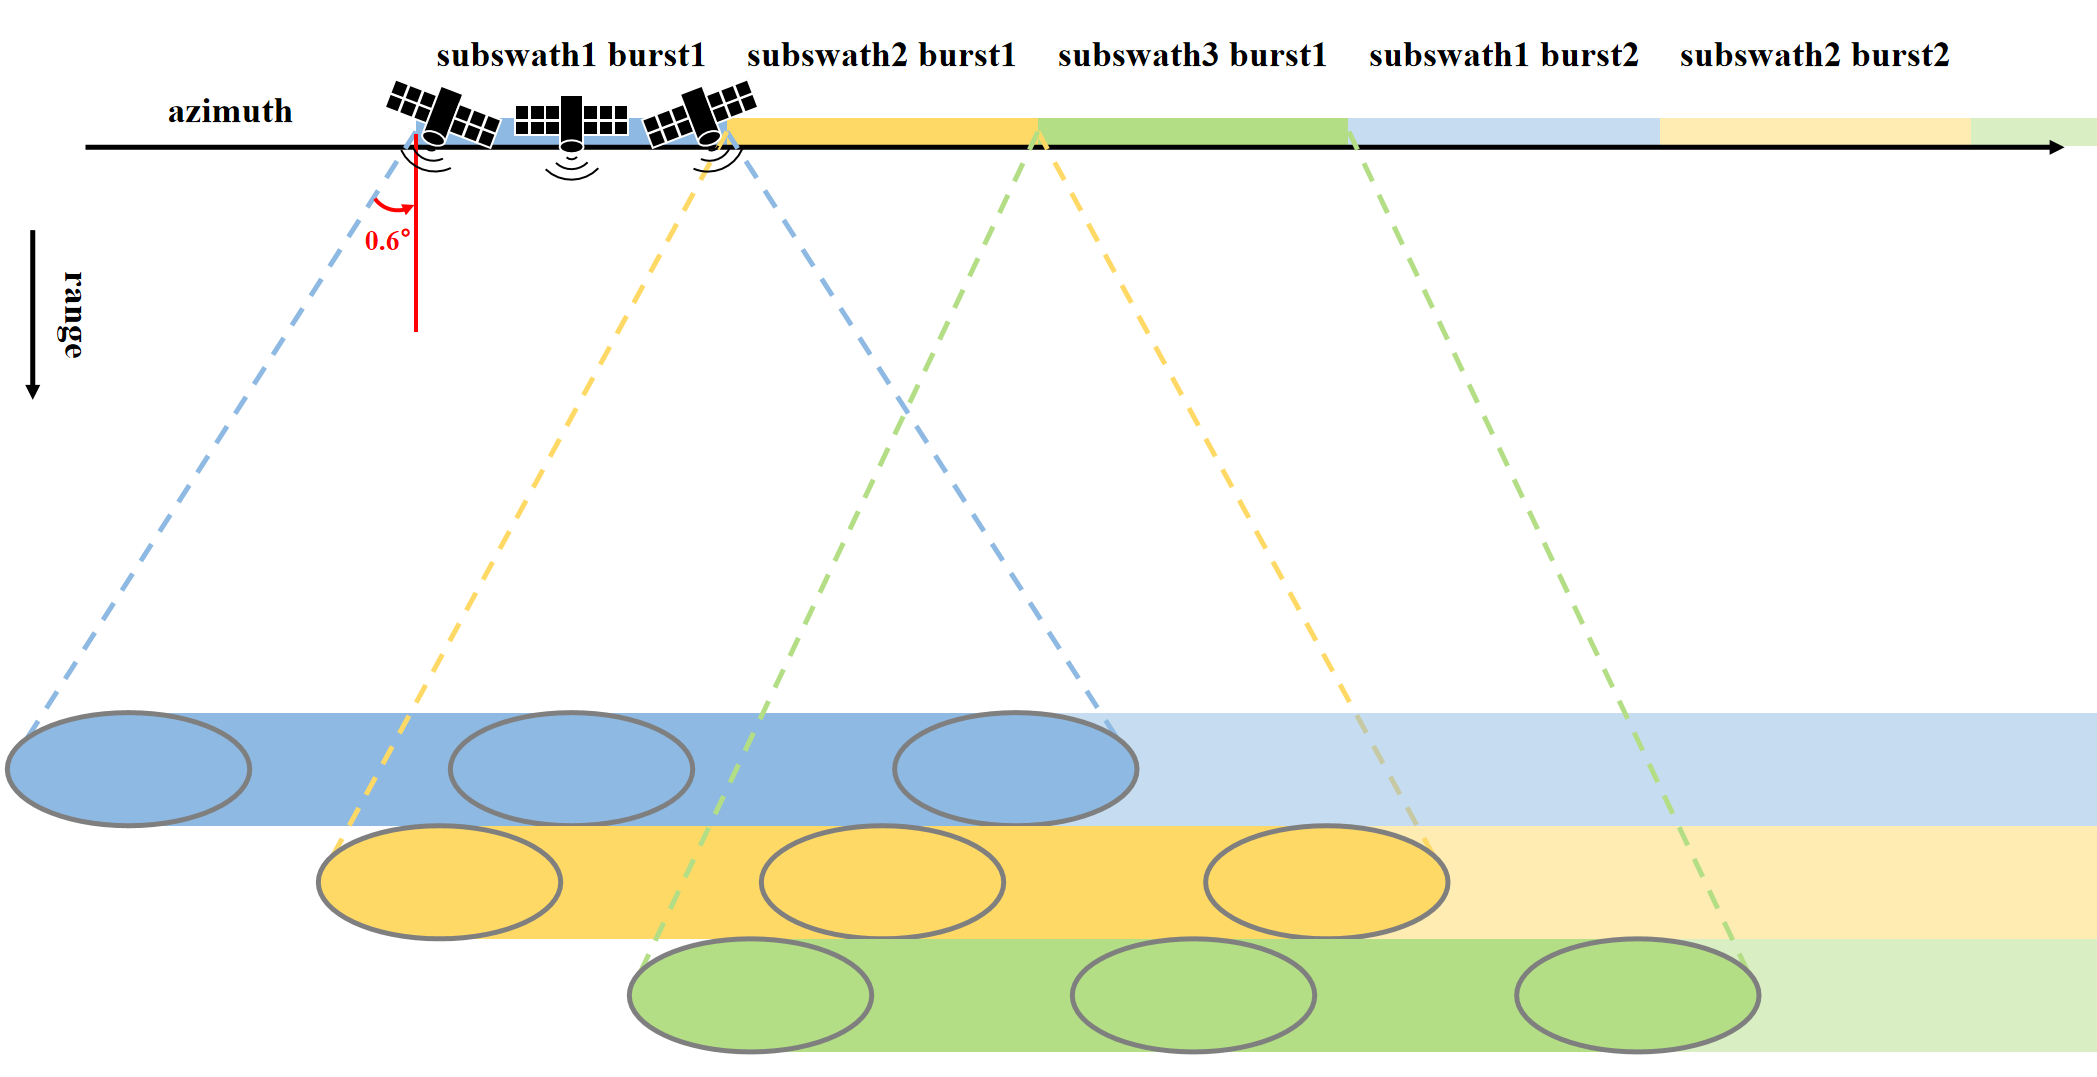
\includegraphics[width=0.8\textwidth]{figure/TOPS Scan pattern for S-1 IW mode.png}	
	\caption{TOPS Scan pattern for S-1 IW mode} 
	\label{fig_1}%
\end{figure}

\begin{table}[htbp]
\caption{SLC product parameters for S-1 IW mode}
\label{table_1}
\begin{tabular*}{\tblwidth}{@{\extracolsep{\fill}}p{0.4\linewidth}p{0.5\linewidth}@{}}
\toprule
Name & Value \\ % Table header row
\midrule
Subswath &
\begin{tabular}[t]{@{}p{0.25\linewidth}p{0.25\linewidth}p{0.25\linewidth}@{}}
iw1 & iw2 & iw3 \\
\end{tabular} \\
Incidence angle &
\begin{tabular}[t]{@{}p{0.25\linewidth}p{0.25\linewidth}p{0.25\linewidth}@{}}
32.9° & 38.3° & 43.1° \\
\end{tabular} \\
Doppler centroid span &
\begin{tabular}[t]{@{}p{0.25\linewidth}p{0.25\linewidth}p{0.25\linewidth}@{}}
5.2kHz & 4.4kHz & 4.6kHz \\
\end{tabular} \\
Azimuth pixel spacing & 14.1m \\
Azimuth sampling frequency & 486.49Hz \\
Squint angle & 0.6° \\
Burst length & 2.75s \\
Ground swath width & 250km \\
Slice length & 170km \\
Orbit height & 689-726km \\
Wavelength & 5.547cm \\
\bottomrule
\end{tabular*}
\end{table}

The miscoregistration time  between the master image and the slave image causes the azimuth phase slope to be \cite{Interferometric_Processing_of_Sentinel-1_TOPS_Data}:\par

\begin{equation}
    \Delta \phi_{\rm az} = 2 \pi \Delta f_{\rm DC} \Delta t = 2 \pi \Delta f_{\rm DC} \frac{\Delta x}{f_{\rm az}}
    \label{eq_1}
\end{equation}

\noindent where $\Delta f_{\rm DC}$ is Doppler centroid span over azimuth, $f_{\rm az}$ is azimuth sampling frequency, and $\Delta x$ is the pixel miscoregistration. In order to limit the phase slope, it is necessary to control the phase deviation at 1\%, that is, 3.6° (or 0.0628 radian) \cite{Interferometric_Processing_of_Sentinel-1_TOPS_Data}. The phase error of 0.0628 radian is transmitted to the deformation error of 0.027cm, which can be ignored for millimeter-level deformation monitoring. In the case of ideal vertical baseline, the phase error of 0.0628 radian is transmitted to the elevation error of tens of centimeters \cite{Effects_of_Phase_Error_on_the_Relative_Height_Accuracy_in_Interferometric_Synthetic_Aperture_Radar}, which can be ignored for meter-level elevation monitoring. Therefore, the phase deviation is controlled within 1\%, which meets the measurement accuracy requirements. Taking the maximum  of 5.2kHz, the miscoregistration time is 1.92$\rm\mu$s. Taking Azimuth sampling frequency of 486.49 Hz, the miscoregistration time is converted to 0.001 pixel. \par

\subsection{ESD}

The S-1 TOPS mode uses the ESD for high-precision coregistration, as shown in \ref{fig_2}. The S-1 TOPS mode has about 7\% to 8\% overlap between adjacent bursts in the azimuth direction. The target is observed twice in the overlap area, then the cross-interferogram is: \par

\begin{equation}
    (m_1 \cdot s_1^*) \cdot (m_2 \cdot s_2^*)^* = {\rm exp} \{j 2 \pi K (t_1 - t_2) \Delta t \}
    \label{eq_2}
\end{equation}

\noindent where $m_1$, $s_1$, $m_2$ and $s_2$ are the master image and slave image at time $t_1$ and $t_2$, respectively; $K$ is the Doppler centroid rate, and $\Delta t$ is miscoregistration time. From \ref{eq_1} and \ref{eq_2}, the ESD phase is: \par

\begin{equation}
    \phi_{\rm ESD} = 2 \pi K (t_1 - t_2) \Delta t = 2 \pi \Delta f_{\rm DC}^{\rm overlap} \frac{\Delta x}{f_{\rm az}}
    \label{eq_3}
\end{equation}

\noindent where $\Delta f_{\rm DC}^{\rm overlap}$ is the Doppler centroid span in the overlap area. In this way, the unique value of $\Delta x$ can be obtained through observations and satellite parameters. \par

\begin{figure}
	\centering 
	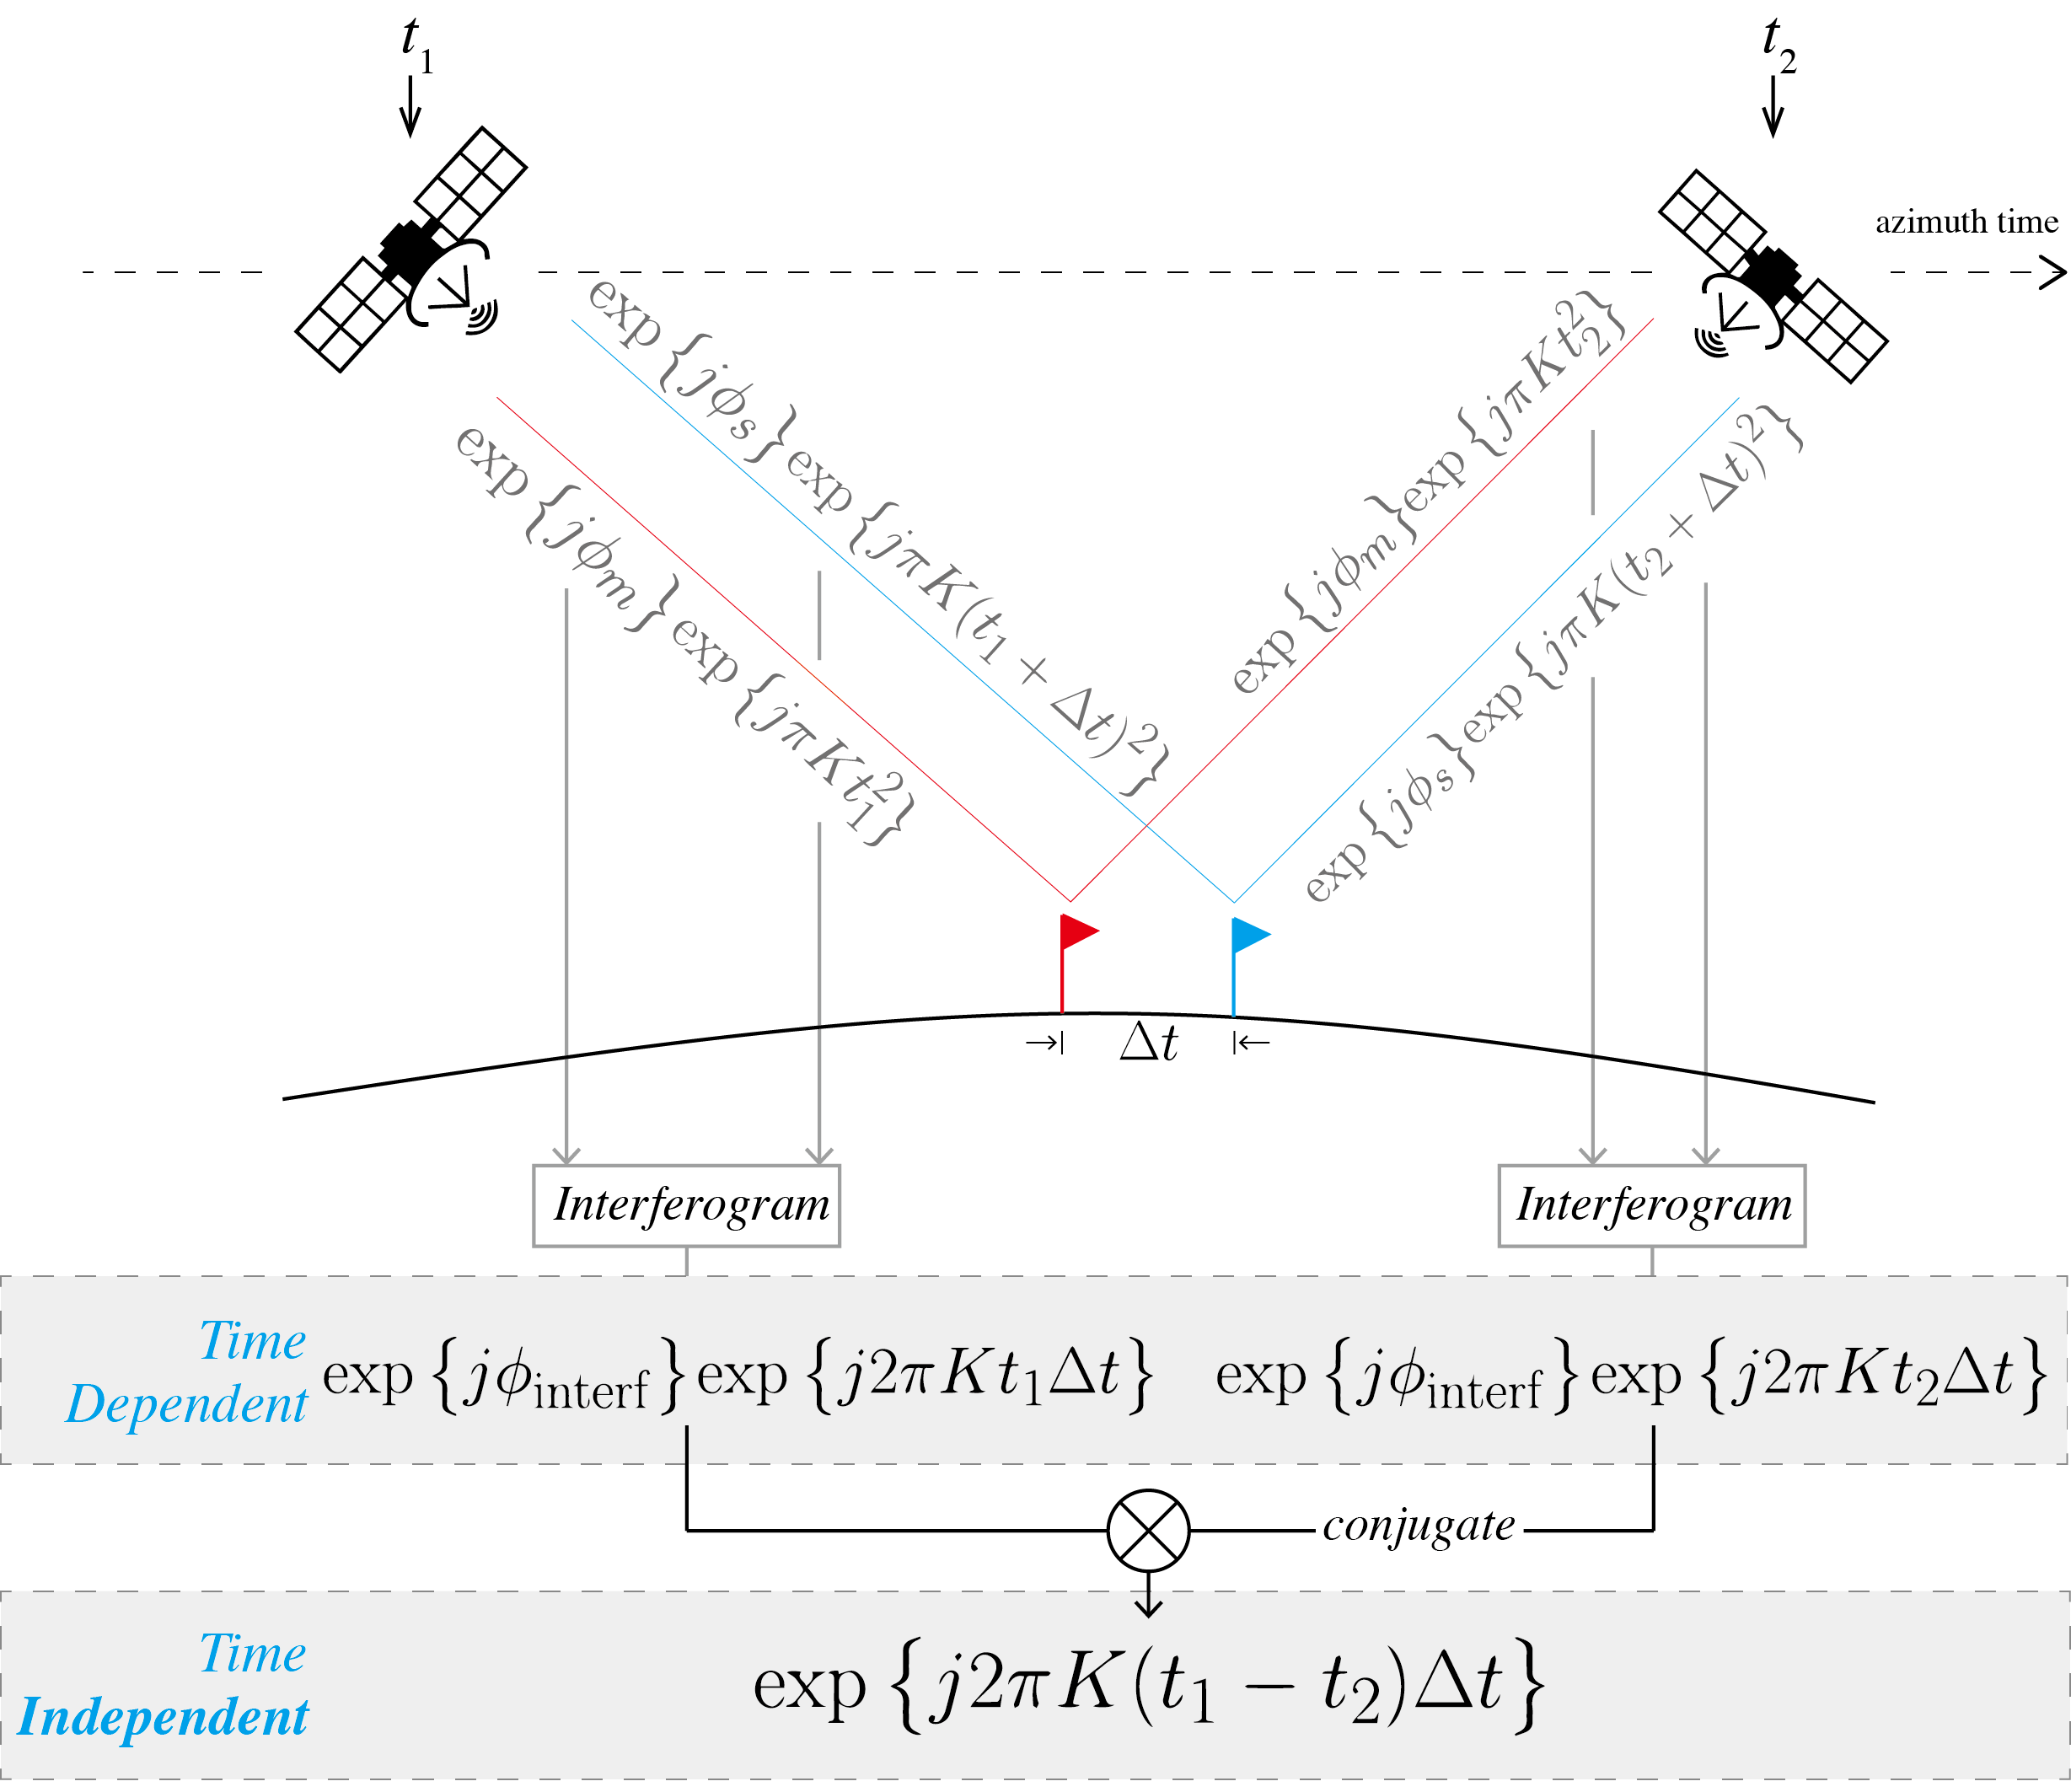
\includegraphics[width=0.6\textwidth]{figure/The principle of ESD.png}	
	\caption{The principle of ESD} 
	\label{fig_2}%
\end{figure}

The azimuth shift phase calculated by the ESD is used to correct the slave image. First, it is transferred to the frequency domain by Fast Fourier Transform (FFT) and rotated in the frequency domain. Then, the inverse FFT is transferred to the spatial domain, and the shift value is remapped to the spatial domain. The calculation formula for shifting the real and imaginary parts of the slave image is: \par

\begin{equation}
    {\rm real} = {\rm real}_0 \cdot {\rm real}_{\Delta x} - {\rm imag}_0 \cdot {\rm imag}_{\Delta x}
    \label{eq_4}
\end{equation}

\begin{equation}
    {\rm imag} = {\rm real}_0 \cdot {\rm imag}_{\Delta x} + {\rm imag}_0 \cdot {\rm real}_{\Delta x}
    \label{eq_5}
\end{equation}

\noindent where ${\rm real}_0$ and ${\rm imag}_0$ are the real and imaginary parts of the original slave image, ${\rm real}_{\Delta x}$ and ${\rm imag}_{\Delta x}$ are the real and imaginary parts of the shift phase. This is the process of signal resampling. Creating a new sample based on a sample with an excessive amount of data consumes a lot of computing power and time. Experimental statistics show that in the operating environment with memory of 180G and parallelism of 56, the ESD processing time of a pair of master image and slave image with size of (subswath*1)*(burst*9) is about 60 seconds, accounting for about 40\% of the entire interference experiment. This experiment is carried out on a higher-configured server. It can be imagined that computing on a generally configured computer will consume more time and computing costs. \par

From \ref{eq_3}, when ignoring the covariance between the two bursts and assuming that the variances of the two bursts are similar, the accuracy of the ESD estimated miscoregistration is: \par

\begin{equation}
    \sigma_{\Delta x} = \frac{\sqrt{2} f_{\rm az} \sigma_\phi}{2 \pi \Delta f_{\rm DC}^{\rm overlap}}
    \label{eq_6}
\end{equation}

\noindent where $\sigma_\phi$ is the phase noise standard deviation, can be approximated as: \par

\begin{equation}
    \sigma_{\phi} = \frac{1}{\sqrt{2N}} \frac{\sqrt{1 - \gamma^2}}{\gamma}
    \label{eq_7}
\end{equation}

\noindent where $N$ is the number of independent averaged samples and $\gamma$ is the interferometric coherence. Relevant research gives the results of the relationship between ESD miscoregistration accuracy and coherence under different sample sizes \cite{A_Network-Based_Enhanced_Spectral_Diversity_Approach_for_TOPS_Time-Series_Analysis}.

\subsection{The Relationship between Geometrical Coregistration Accuracy and Orbit Accuracy}
The essence of geometrical coregistration is to map the master image and slave image to the Cartesian coordinate system by means of satellite orbit information and external digital elevation model (DEM), and then calculate the shift according to the Cartesian coordinate to achieve coregistration. Geometrical coregistration does not rely on coherence, and the coregistration accuracy can be satisfied with the help of external data. Therefore, in fact, the residual error after geometrical coregistration is a constant displacement, which mainly comes from the orbital error. The coregistration error in the azimuth is expressed as \cite{Geometrical_SAR_image_registration}: \par

\begin{equation}
    \delta_{\rm az} = \hat{v} \cdot \frac{\delta_{S_0}}{\Delta^{({\rm az})}}
    \label{eq_8}
\end{equation}

\noindent where $\hat{v}$ is the velocity unit vectors for master image, $\Delta^{({\rm az})}$ is the azimuth sampling spacing (in meters) for master image, and $S_0$ is the shift along the orbital direction between master orbit and slave orbit. This means that the geometrical coregistration error is proportional to the shift along the orbital direction. \par
The precise orbit data provided by European Space Agency (ESA) can control the absolute positioning accuracy of satellite orbit within 5 cm. The orbit evaluation results of S-1 A satellite from 2019 to 2022 are shown in \ref{table_2} \cite{copernicus_review_2015.10-2019.09, copernicus_review_2019.10-2020.01, copernicus_review_2020.02-2020.05, copernicus_review_2020.06-2020.09, copernicus_review_2020.10-2020.12, copernicus_review_2021.01-2021.12, copernicus_review_2022.01-2022.12}. The precision index is the 3D RMS (Root Mean Square) between the Copernicus Precise Orbit Determination (CPOD) and the joint orbit products generated by other institutions. It is noted that the large error from 2019 to 2020 is mainly due to the updated Antenna Reference Point (ARP) and ANTEX (Antenna Exchange Format) configurations used by other institutions. In July 2020, after the ESA approved the update of the S-1 A CPOD configuration, the accuracy met the requirements and gradually became more optimized. \par

\begin{table}[htbp]
\caption{Estimated accuracy of S1-A satellite CPOD products}
\label{table_2}
\raggedright % 表格左对齐
\begin{tabular}{p{0.2\linewidth}p{0.2\linewidth}}
\toprule
Date & 3D RMS(cm) \\ % Table header row
\midrule
2019.02-2019.05 & 1.44 \\
2019.06-2019.09 & 6.29 \\
2019.10-2020.01 & 6.36 \\
2020.02-2020.05 & 6.37 \\
2020.06-2020.09 & 4.18 \\
2020.10-2020.12 & 1.46 \\
2021.01-2021.12 & 0.48 \\
2022.01-2022.12 & 0.60 \\
\bottomrule
\end{tabular}
\end{table}

From \ref{eq_8}, assuming that master orbit and slave orbit are independent, the geometrical coregistration accuracy in the azimuth can be expressed as: \par

\begin{equation}
    \sigma_{\rm az} = \sqrt{\sigma_m^2 + \sigma_s^2}
    \label{eq_9}
\end{equation}

\noindent where $\sigma_m$ and $\sigma_s$ are the accuracy of master orbit and slave orbit. The RMS of the SAR satellite orbit in the report is used as the estimation of $\sigma_m$ and $\sigma_s$ \cite{InSAR_uncertainty_due_to_orbital_errors}. Then, taking the 3D RMS of the track as 1.5cm, the geometrical coregistration accuracy will be better than 2.12cm. From \ref{table_1}, the azimuth pixel sampling is 14.1m, and the geometrical coregistration accuracy can be converted to 0.0015 pixel. \par


\section{Method}

\subsection{The Master Image Correction Method}

Coregistration is a relative process in which the corresponding points of the master and slave image correspond to the same resolution unit. From \ref{eq_8}, it can be seen that the geometrical coregistration error is proportional to the shift along the orbital direction between master orbit and slave orbit. There is a set of SAR images, and the geometrical coregistration error range is: \par

\begin{equation}
    \mu_m \pm \sigma
    \label{eq_10}
\end{equation}

\noindent where $\mu_m$ is the coregistration error of the master image along the track direction, and $\sigma$ is the degree of dispersion of all slave images relative to the master image. If only the master image is corrected with high precision, the coregistration error of the slave image can be ignored. The geometrical coregistration error is: \par

\begin{equation}
    \sigma_{\rm az} = \sigma
    \label{eq_11}
\end{equation}

\noindent Therefore, when the orbit control of the slave image is good, only the correction of the master image after geometrical coregistration can meet the requirements of high-precision coregistration. \par

\subsection{The Coregistration Method Based on Phase without Resampling}

According to the TOPS impulse response function, assuming that the beam-center time $t_c$ is 0, the phase difference between the master image and slave image is: \par

\begin{equation}
\begin{split}
s_s(t + \Delta t) \cdot s_m^*(t) = & s_{a, s}(t + \Delta t) \cdot s_{a, m}(t)  \\
& \cdot {\rm exp} \{-j \frac{4 \pi}{\lambda} \Delta R\} \cdot {\rm exp} \{j 2 \pi K t \Delta t\} \\
& \cdot {\rm exp} \{ j \pi K \Delta t^2\}
\end{split}
\label{eq_12}
\end{equation}

\noindent where $s_a$ is amplitude function, and $t$ is the azimuth zero Doppler time. In general, the value of the miscoregistration time $\Delta t$ is very small, so the changes of $s_a$ and ${\rm exp} \{ j \pi K \Delta t^2\}$ can be ignored. Thus, the following can be obtained: \par

\begin{equation}
    s_s(t + \Delta t) \cdot s_m^*(t) = {\rm exp} \{-j \frac{4 \pi}{\lambda} \Delta R\} \cdot {\rm exp} \{j 2 \pi K t \Delta t\}
    \label{eq_13}
\end{equation}

\noindent There is an observation $s_s(t + \Delta t) \cdot s_m^*(t)$ and two unknowns $\Delta R$ and $\Delta t$. When another measurement is performed, two observations are obtained, and the unique solution of the two unknowns can be solved. \par
Bring \ref{eq_3} into \ref{eq_13}, for a single image can be obtained: \par

\begin{equation}
    s(t) = s(t + \Delta t) \cdot {\rm exp} \{-j \phi_{\rm ESD} \frac{t}{t_1 - t_2}\}
    \label{eq_14}
\end{equation}

\noindent From \ref{eq_14}, the coregistration can be completed by the product of the miscoregistration image and the function of the azimuth time. In theory, ESD does not need to resample to correct the miscoregistration time $\Delta t$, which greatly improves the computational efficiency. \par


\section{Experiment}

The S-1 IW TOPS mode is affected by the change of Doppler frequency, and requires a coregistration accuracy of at least 0.001 pixel. In recent years, the official report of ESA shows that the 3D RMS of the precise orbit data has been better than 1.5cm. In theory, the geometrical coregistration accuracy can meet 0.0015 pixel, and there is no need for ESD secondary resampling. Therefore, this section conducts experimental research. The main purpose is to explore whether the residual error after coregistration of precise orbit data with higher precision is within an acceptable range, and to judge the necessity of ESD. \par

Based on background investigation and theoretical analysis, the factors that need to be considered in the experiment are divided into three categories. The first category is the study area, including the study area with different coherence and the study area located at different latitudes. The second category is SAR data, including ascending or descending, and different numbers of bursts. The third category is precise orbit data, including data before adjustment configuration from 2019 to 2020, data updated after adjustment configuration from 2019 to 2020, and data with higher precision from 2022 to 2023. The above different factors were compared, and Shuttle Radar Topography Mission (SRTM) 30m was used as external DEM data. Since the accuracy of ESD coregistration is very high, the ESD result is used as the reference value of the ‘true value’ in this experiment. Therefore, the azimuth shift difference and phase deviation between the geometrical coregistration result and the reference value are used as the quantitative evaluation indexes of the residual error, and the cross-interferogram between the geometrical coregistration result and the reference value is used as the qualitative evaluation index of the residual error. The experimental design was two groups, as shown in \ref{fig_3}. \par

\begin{figure}
	\centering 
	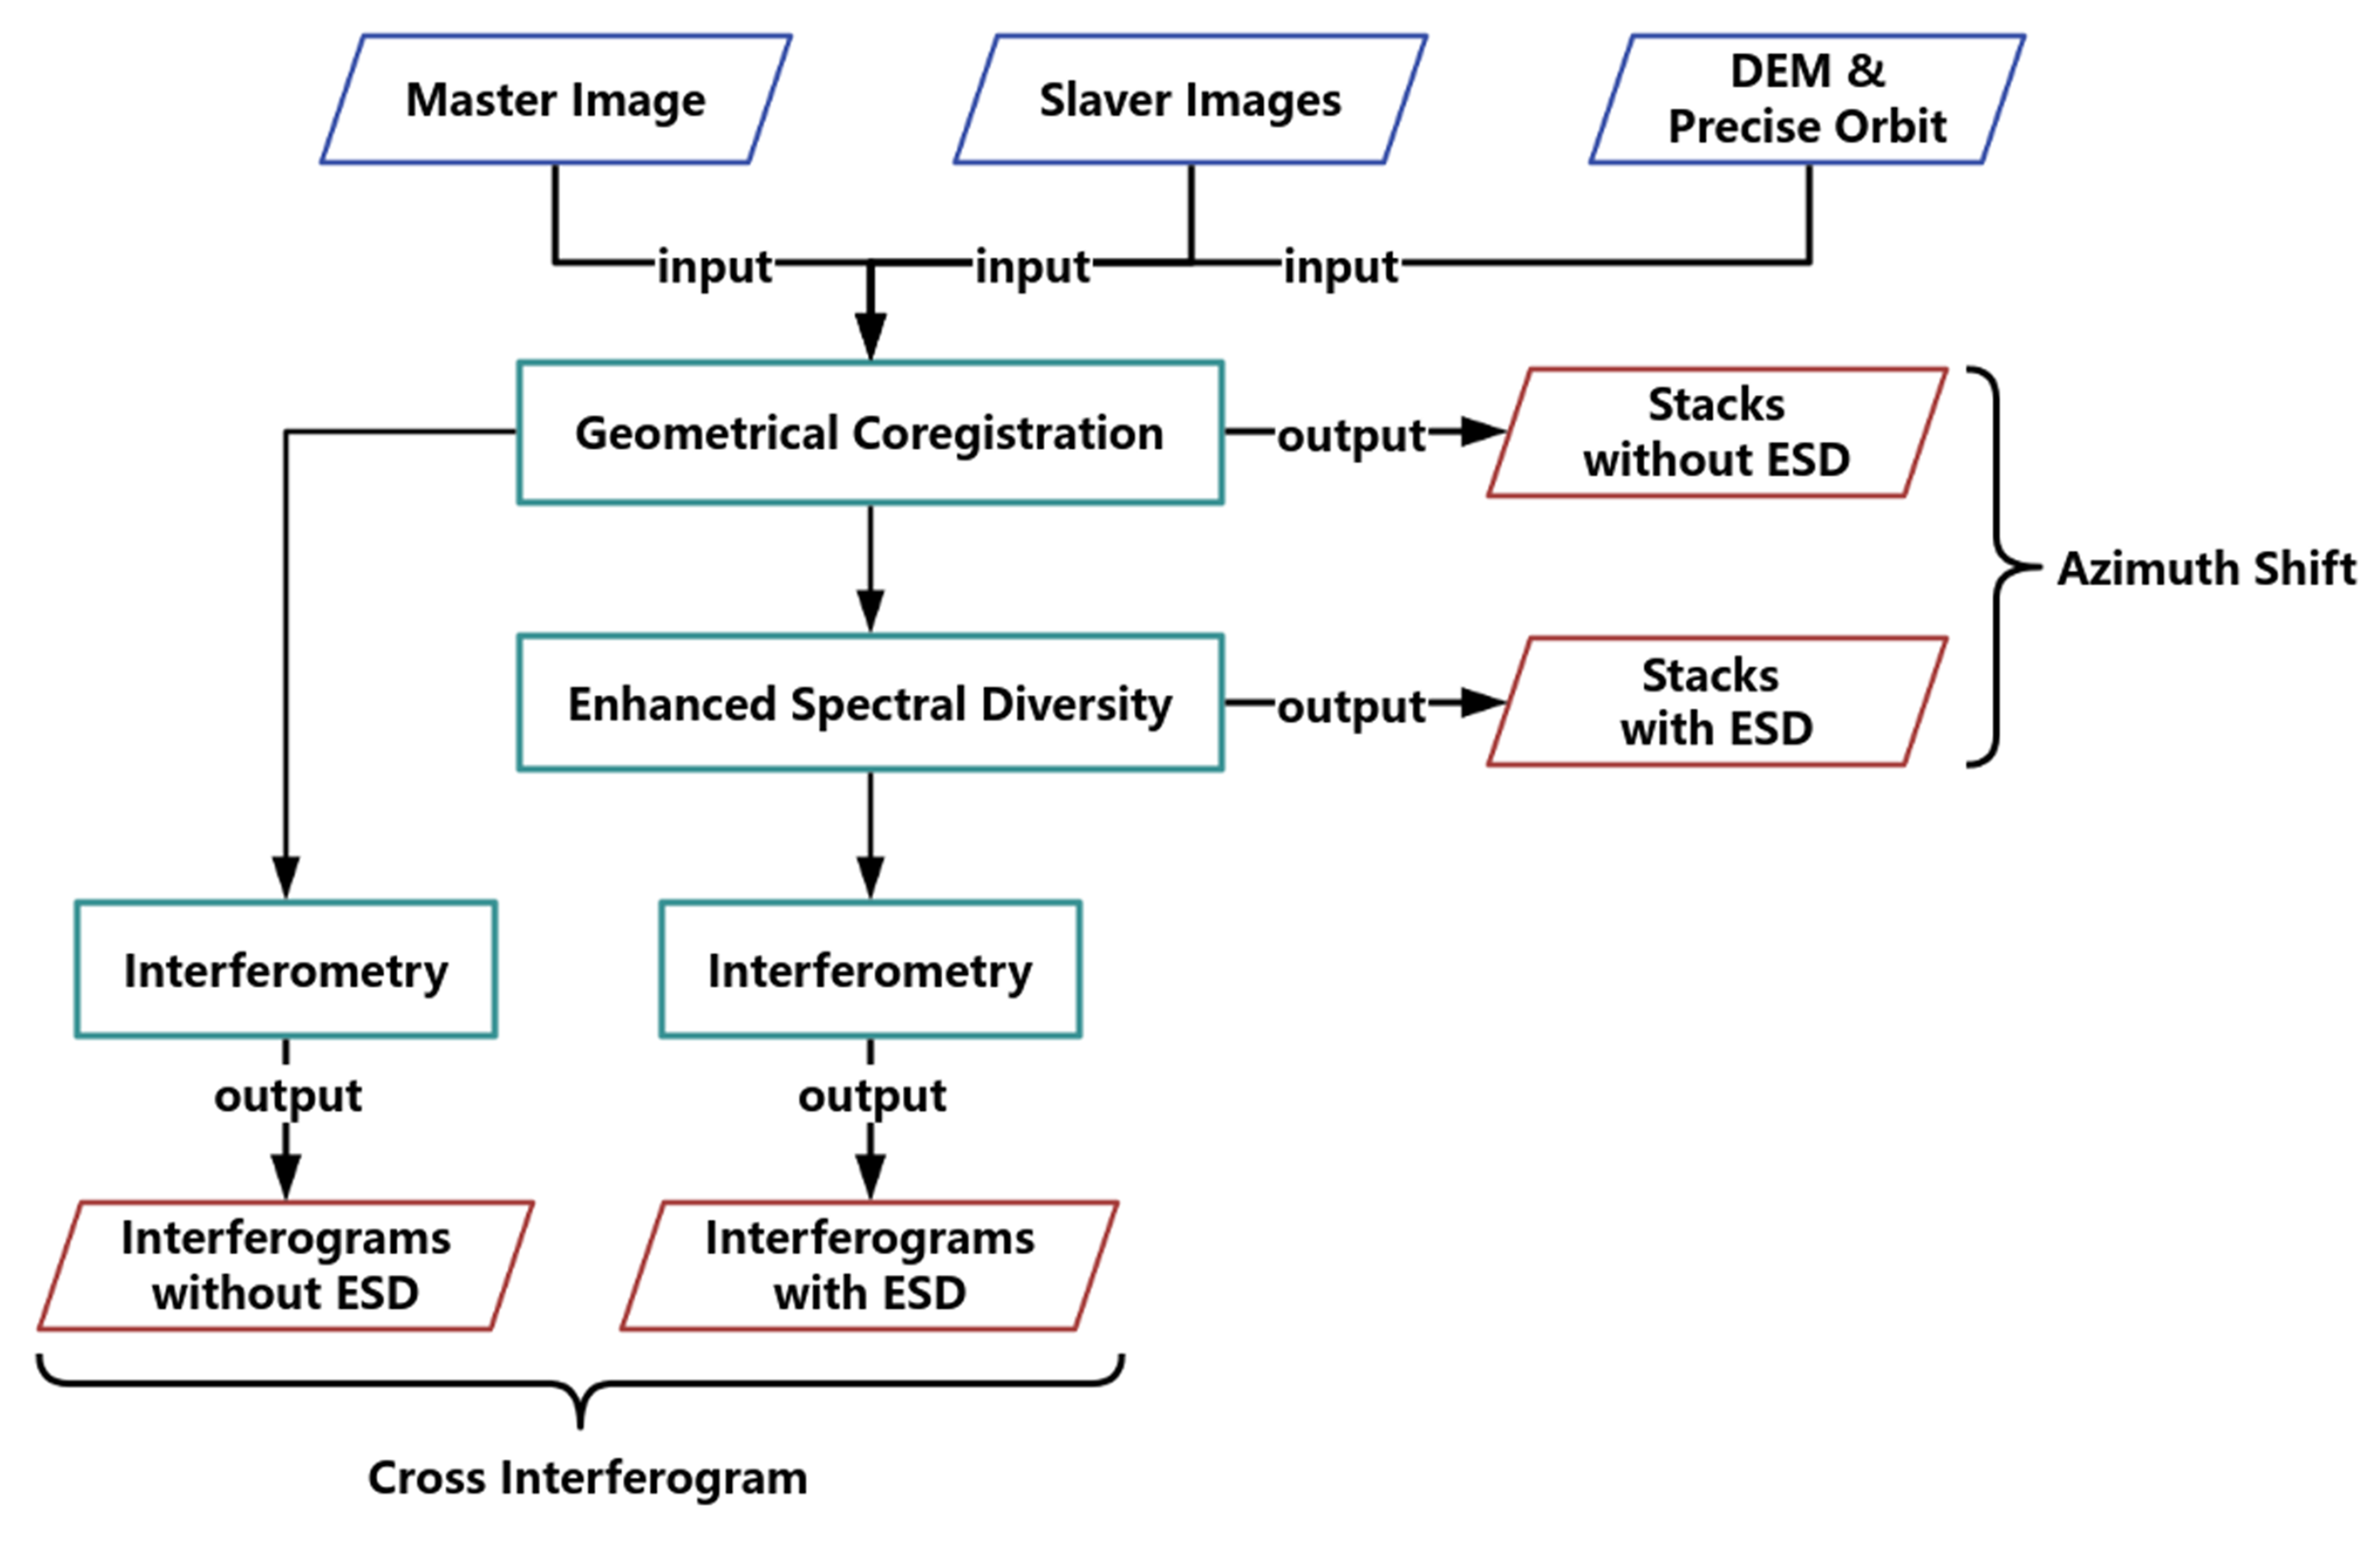
\includegraphics[width=0.7\textwidth]{figure/Experimental flow chart.png}	
	\caption{Experimental flow chart} 
	\label{fig_3}%
\end{figure}

\subsection{Data}

According to the principle of statistical universality, the experiments in this section select five research areas with different correlations and located in different latitudes, including the regions of Taklamakan Desert, Mexico City, Xi’an, Milan and Finland. SAR data covering the above five research areas are shown in \ref{fig_4} (the SAR data of different coverage areas are represented by the name of the study area). The properties of data are shown in \ref{table_3}. The monitoring time includes two periods, from May 2019 to September 2020 and from January 2022 to December 2023. \par

\begin{figure}
    \centering
    \begin{subfigure}{0.32\textwidth}
        \centering
        \includegraphics[width=\textwidth]{figure/SAR data coverage/TaklimakanDesert.png}
        \caption{Taklamakan desert}
        \label{fig_4a}
    \end{subfigure}%
    \begin{subfigure}{0.32\textwidth}
        \centering
        \includegraphics[width=\textwidth]{figure/SAR data coverage/Mexico.png}
        \caption{Mexico City}
        \label{fig_4b}
    \end{subfigure}
    \begin{subfigure}{0.32\textwidth}
        \centering
        \includegraphics[width=\textwidth]{figure/SAR data coverage/XiAn.png}
        \caption{XiAn}
        \label{fig_4c}
    \end{subfigure}
    \medskip
    \begin{subfigure}{0.32\textwidth}
        \centering
        \includegraphics[width=\textwidth]{figure/SAR data coverage/Milan.png}
        \caption{Milan}
        \label{fig_4d}
    \end{subfigure}%
    \begin{subfigure}{0.32\textwidth}
        \centering
        \includegraphics[width=\textwidth]{figure/SAR data coverage/Finland.png}
        \caption{Finland}
        \label{fig_4e}
    \end{subfigure}
    \caption{SAR data coverage}
    \label{fig_4}
\end{figure}

\begin{table}[htbp]
\caption{The properties of SAR data}
\label{table_3}
% \begin{tabular*}{\tblwidth}{@{\extracolsep{\fill}}p{0.16\linewidth}p{0.13\linewidth}p{0.18\linewidth}p{0.05\linewidth}p{0.05\linewidth}p{0.1\linewidth}p{0.11\linewidth}@{}}
\begin{tabular*}{\tblwidth}{@{\extracolsep{\fill}}ccccccc@{}}
\toprule
Area & Flight Direction & Start Date - End Date & Path & Frame & IW \& Burst & Polarization \\ % Table header row
\midrule
\multirow{4}{*}{\centering Taklamakan desert} & \multirow{2}{*}{\centering Ascending} & 2019.05 - 2020.09 & \multirow{2}{*}{\centering 158} & \multirow{2}{*}{\centering 122} & \multirow{4}{*}{\centering 2 \& 1-9} & \multirow{18}{*}{\centering VV} \\
 &  & 2022.01 - 2023.12 &  &  &  &  \\
 & \multirow{2}{*}{\centering Descending} & 2019.05 - 2020.09 & \multirow{2}{*}{\centering 63} & 464 &  &  \\
 &  & 2022.07 - 2023.11 &  & 463 &  &  \\
\cmidrule{1-6}
\multirow{4}{*}{\centering Mexico City} & \multirow{2}{*}{\centering Ascending} & 2019.05 - 2020.09 & \multirow{2}{*}{\centering 5} & \multirow{2}{*}{\centering 57} & \multirow{2}{*}{\centering 1 \& 6-8} &  \\
 &  & 2022.01 - 2023.12 &  &  &  &  \\
 & \multirow{2}{*}{\centering Descending} & 2019.05 - 2020.09 & \multirow{2}{*}{\centering 41} & \multirow{2}{*}{\centering 528} & \multirow{2}{*}{\centering 1 \& 1-3} &  \\
 &  & 2022.01 - 2023.12 &  &  &  &  \\
\cmidrule{1-6}
\multirow{2}{*}{\centering Xi'an} & \multirow{2}{*}{\centering Ascending} & 2019.05 - 2020.09 & \multirow{2}{*}{\centering 84} & \multirow{2}{*}{\centering 105} & \multirow{2}{*}{\centering 2 \& 7-9} &  \\
 &  & 2022.01 - 2023.12 &  &  &  &  \\
\cmidrule{1-6}
\multirow{4}{*}{\centering Milan} & \multirow{2}{*}{\centering Ascending} & 2019.05 - 2020.09 & \multirow{2}{*}{\centering 15} & \multirow{2}{*}{\centering 144} & \multirow{2}{*}{\centering 2 \& 4-6} &  \\
 &  & 2022.01 - 2023.12 &  &  &  &  \\
 & \multirow{2}{*}{\centering Descending} & 2019.05 - 2020.09 & \multirow{2}{*}{\centering 66} & \multirow{2}{*}{\centering 439} & \multirow{2}{*}{\centering 1 \& 6-8} &  \\
 &  & 2022.01 - 2023.12 &  &  &  &  \\
\cmidrule{1-6}
\multirow{4}{*}{\centering Filand} & \multirow{2}{*}{\centering Ascending} & 2019.05 - 2020.09 & \multirow{2}{*}{\centering 160} & \multirow{2}{*}{\centering 193} & \multirow{2}{*}{\centering 2 \& 7-9} &  \\
 &  & 2022.01 - 2023.12 &  &  &  &  \\
 & \multirow{2}{*}{\centering Descending} & 2019.05 - 2020.09 & \multirow{2}{*}{\centering 153} & 392 & 2 \& 1-3 &  \\
 &  & 2022.01 - 2023.12 &  & 388 & 2 \& 6-8 &  \\
\bottomrule
\end{tabular*}
\end{table}

Area 1 (\ref{fig_4a}): Taklamakan desert, which belongs to the plateau and has a dry climate. The quality of the overall coherence in the region is uniform, and there are rivers and traffic lines to determine the geographical location of the pixel. It is a relatively ideal test. Area 2 (\ref{fig_4b}): Mexico City, located in low latitudes. In the past 50 years, the process of ‘urbanization’ has been faster \cite{Urban_growth_and_land_subsidence:_Multi-decadal_investigation_using_human_settlement_data_and_satellite_InSAR_in_Morelia_Mexico}. There is also a certain vegetation coverage in the area, but the city is dominant. The coherence is high, which belongs to the city-led test. Area 3 (\ref{fig_4c}): Xi’an, located in the middle latitudes. The city is located in the basin, and the south is close to the Qinling Mountains, which belongs to the test of city and mountain. Area 4 (\ref{fig_4d}): Milan, located in the middle latitudes. Located in Po Valley, the surrounding cities are dense. There are vegetation coverage areas, and the boundary between urban and non-urban areas is obvious, which belongs to the test of urban and vegetation. Area 5 (\ref{fig_4e}): Finland. The region is mainly concentrated in the urban agglomerations of southern Finland, but the forest coverage is very high and the southern coast. The overall coherence is low, which belongs to the vegetation-dominated test. \par

\subsection{Interference Experiment Result and Analysis}

Combined with different considerations, including the study area, satellite flight direction and orbit data, this section established 27 sets of comparative experiments, using 830 images, and actually processing 1179 images. In order to avoid the influence of other operations, this experiment did not carry out optimization steps such as multi-view and filtering. Details of the experimental results are shown in \ref{table_4}. It can be seen that compared the use of different orbit data, although most of the adjusted results have been improved, they are basically on the order of one ten thousandth of a pixel, and there is no significant difference in phase. It is speculated that there may be other reasons, which is discussed in 5 (1). \par

% 该表格考虑加入附件中
% 先保存当前页面的页边距
\newgeometry{left=1cm,right=1cm,top=1cm,bottom=1cm}

\begin{table}[htbp]
\caption{The interference experiment result}
\label{table_4}
\begin{minipage}[t]{\linewidth}
\centering
\begin{tabular*}{\linewidth}{@{\extracolsep{\fill}}>{\centering\arraybackslash}p{0.11\linewidth}>{\centering\arraybackslash}p{0.18\linewidth}*{9}{>{\centering\arraybackslash}p{0.042\linewidth}} }
\toprule
\multicolumn{2}{c}{\centering The serial number of the experiment} & 1 & 2 & 3 & 4 & 5 & 6 & 7 & 8 & 9 \\ % Table header row
\midrule
\multirow{5}{1\linewidth}{\centering Study area} & Taklamakan desert & $\bigcirc$ & $\bigcirc$ & $\bigcirc$ & $\bigcirc$ & $\bigcirc$ & $\bigcirc$ \\
 & Mexico City &  &  &  &  &  &  & $\bigcirc$ & $\bigcirc$ & $\bigcirc$ \\
 & Xi’an \\
 & Milan \\
 & Finland \\
\midrule
\multirow{2}{1\linewidth}{\centering Flight direction} & Ascending & $\bigcirc$ & $\bigcirc$ & $\bigcirc$ &  &  &  & $\bigcirc$ & $\bigcirc$ & $\bigcirc$ \\
 & Descending &  &  &  & $\bigcirc$ & $\bigcirc$ & $\bigcirc$ \\
\midrule
\multirow{3}{1\linewidth}{\centering Orbit data} & Old (2019-2020) &  &  & $\bigcirc$ &  &  & $\bigcirc$ &  &  & $\bigcirc$ \\
 & New (2019-2020) &  & $\bigcirc$ &  &  & $\bigcirc$ &  &  & $\bigcirc$ \\
 & Normal (2022-2023) & $\bigcirc$ &  &  & $\bigcirc$ &  &  & $\bigcirc$ \\
\midrule
\multicolumn{2}{c}{\centering Number of SAR images} & 59 & 43 & 43 & 34 & 8 & 8 & 60 & 43 & 43 \\
\midrule
Shift & Mean value & -0.31 & -0.36 & 0.21 & -0.30 & 0.28 & 0.43 & 2.78 & -0.51 & 0.46 \\
($*10^{-3}$ pixel) & Standard deviation & 1.07 & 0.98 & 1.14 & 0.77 & 1.14 & 1.10 & 2.86 & 2.12 & 2.37 \\
\midrule
\multirow{2}{1\linewidth}{\centering Phase bias (radian)} & Mean value & -0.02 & -0.02 & 0.01 & -0.02 & 0.02 & 0.02 & 0.19 & -0.03 & 0.03 \\
 & Standard deviation & 0.06 & 0.06 & 0.06 & 0.04 & 0.06 & 0.06 & 0.19 & 0.14 & 0.16 \\
\bottomrule
\end{tabular*}
\end{minipage}

\vspace{0.1cm}

\begin{minipage}[t]{\linewidth}
\centering
\begin{tabular*}{\linewidth}{@{\extracolsep{\fill}}>{\centering\arraybackslash}p{0.11\linewidth}>{\centering\arraybackslash}p{0.18\linewidth}*{9}{>{\centering\arraybackslash}p{0.042\linewidth}} }
\toprule
\multicolumn{2}{c}{\centering The serial number of the experiment} & 10 & 11 & 12 & 13 & 14 & 15 & 16 & 17 & 18 \\ % Table header row
\midrule
\multirow{5}{1\linewidth}{\centering Study area} & Taklamakan desert \\
 & Mexico City & $\bigcirc$ & $\bigcirc$ & $\bigcirc$ \\
 & Xi’an &  &  &  & $\bigcirc$ & $\bigcirc$ & $\bigcirc$ \\
 & Milan &  &  &  &  &  &  & $\bigcirc$ & $\bigcirc$ & $\bigcirc$ \\
 & Finland \\
\midrule
\multirow{2}{1\linewidth}{\centering Flight direction} & Ascending &  &  &  & $\bigcirc$ & $\bigcirc$ & $\bigcirc$ & $\bigcirc$ & $\bigcirc$ & $\bigcirc$ \\
 & Descending & $\bigcirc$ & $\bigcirc$ & $\bigcirc$ \\
\midrule
\multirow{3}{1\linewidth}{\centering Orbit data} & Old (2019-2020) &  &  & $\bigcirc$ &  &  & $\bigcirc$ &  &  & $\bigcirc$ \\
 & New (2019-2020) &  & $\bigcirc$ &  &  & $\bigcirc$ &  &  & $\bigcirc$ \\
 & Normal (2022-2023) & $\bigcirc$ &  &  & $\bigcirc$ &  &  & $\bigcirc$ \\
\midrule
\multicolumn{2}{c}{\centering Number of SAR images} & 55 & 42 & 42 & 33 & 42 & 42 & 61 & 44 & 44 \\
\midrule
Shift & Mean value & -3.25 & 0.61 & 1.27 & 4.88 & 2.06 & 2.47 & -1.02 & -5.35 & -5.64 \\
($*10^{-3}$ pixel) & Standard deviation & 2.30 & 1.70 & 1.49 & 3.26 & 2.21 & 2.25 & 1.80 & 1.78 & 2.20 \\
\midrule
\multirow{2}{1\linewidth}{\centering Phase bias (radian)} & Mean value & -0.22 & 0.04 & 0.09 & 0.28 & 0.12 & 0.14 & -0.06 & -0.30 & -0.32 \\
 & Standard deviation & 0.15 & 0.11 & 0.10 & 0.19 & 0.13 & 0.13 & 0.10 & 0.10 & 0.13 \\
\bottomrule
\end{tabular*}
\end{minipage}

\vspace{0.1cm}

\begin{minipage}[t]{\linewidth}
\centering
\begin{tabular*}{\linewidth}{@{\extracolsep{\fill}}>{\centering\arraybackslash}p{0.11\linewidth}>{\centering\arraybackslash}p{0.18\linewidth}*{9}{>{\centering\arraybackslash}p{0.042\linewidth}} }
\toprule
\multicolumn{2}{c}{\centering The serial number of the experiment} & 19 & 20 & 21 & 22 & 23 & 24 & 25 & 26 & 27 \\ % Table header row
\midrule
\multirow{5}{1\linewidth}{\centering Study area} & Taklamakan desert \\
 & Mexico City \\
 & Xi’an \\
 & Milan & $\bigcirc$ & $\bigcirc$ & $\bigcirc$ \\
 & Finland &  &  &  & $\bigcirc$ & $\bigcirc$ & $\bigcirc$ & $\bigcirc$ & $\bigcirc$ & $\bigcirc$ \\
\midrule
\multirow{2}{1\linewidth}{\centering Flight direction} & Ascending &  &  &  & $\bigcirc$ & $\bigcirc$ & $\bigcirc$ \\
 & Descending & $\bigcirc$ & $\bigcirc$ & $\bigcirc$ &  &  &  & $\bigcirc$ & $\bigcirc$ & $\bigcirc$ \\
\midrule
\multirow{3}{1\linewidth}{\centering Orbit data} & Old (2019-2020) &  &  & $\bigcirc$ &  &  & $\bigcirc$ &  &  & $\bigcirc$ \\
 & New (2019-2020) &  & $\bigcirc$ &  &  & $\bigcirc$ &  &  & $\bigcirc$ \\
 & Normal (2022-2023) & $\bigcirc$ &  &  & $\bigcirc$ &  &  & $\bigcirc$ \\
\midrule
\multicolumn{2}{c}{\centering Number of SAR images} & 60 & 42 & 42 & 60 & 42 & 42 & 59 & 43 & 43 \\
\midrule
Shift & Mean value & -4.57 & -2.81 & -3.87 & 0.55 & -2.82 & -2.91 & 0.06 & 2.43 & 1.67 \\
($*10^{-3}$ pixel) & Standard deviation & 2.13 & 2.08 & 1.95 & 2.99 & 2.46 & 2.73 & 3.81 & 2.00 & 1.99 \\
\midrule
\multirow{2}{1\linewidth}{\centering Phase bias (radian)} & Mean value & -0.31 & -0.19 & -0.26 & 0.03 & -0.16 & -0.17 & 0.00 & 0.14 & 0.10 \\
 & Standard deviation & 0.14 & 0.14 & 0.13 & 0.17 & 0.14 & 0.15 & 0.22 & 0.11 & 0.11 \\
\bottomrule
\end{tabular*}
\end{minipage}
\end{table}

% 恢复原始的页面页边距
\restoregeometry

Assuming that the interferograms are independent, the azimuth shift difference and phase deviation of all images are calculated by taking the proportion of interferograms as the weight. The statistical result of the difference between the azimuth shift is -0.63±2.12 ($*10^{-3}$) pixel, and the phase deviation is -0.04±0.13 radian. In theory, since geometrical coregistration is mainly affected by the orbit, the coregistration of enough SAR data is in line with the standard normal distribution. However, due to the limitation of data, the mean is not zero. The mean value of the individual results involves a large range, about -0.005 to 0.005 pixel, while the standard deviation is about 0.002 pixel. Considering that coregistration is a relative process, we use the mean as the positioning error of the master image and the standard deviation as the coregistration error of the slave images. If the master image error can be corrected, the coregistration accuracy of the lave images is about 0.002 pixel without correction. The overall result meets the absolute positioning accuracy of 1.5 cm for a single scene image, but there is a difference of about 0.001 pixel with the relative accuracy of coregistration and the coregistration requirements of TOPS mode. The error is discussed in 5 (2). \par

The results of interference experiments from January 2022 to January 2023 are taken as reference. The cross-interferogram between interferogram without ESD and interferogram with ESD is shown in \ref{fig_5}. Theoretically, the constant deviation in the direction of azimuth should not affect the difference in the direction of range. Therefore, with coherence as the weight, the weighted average of the range is obtained and visualized (blue line), and the least squares fitting (red line) is performed for each change. The results are shown in \ref{fig_5}. It can be clearly seen that the phase changes periodically in the unit of burst. Overall, most phase deviations are between -0.15 and 0.15 radian. It is found that the noise level is very high in the Taklamakan desert ascending (\ref{fig_5a}), and even an ‘unknown’ trend in the distance direction appears in the cross-interferogram. The phase loss in overlap was found in the Finland ascending (\ref{fig_5h}), which is caused by water incoherence. The above two cases will inevitably affect the calculation of ESD phase, and lead to coregistration errors. \par

\begin{figure}
    \centering
    \begin{subfigure}[c]{0.5\textwidth}
        \centering
        \begin{minipage}[c]{0.5\textwidth}
            \centering
            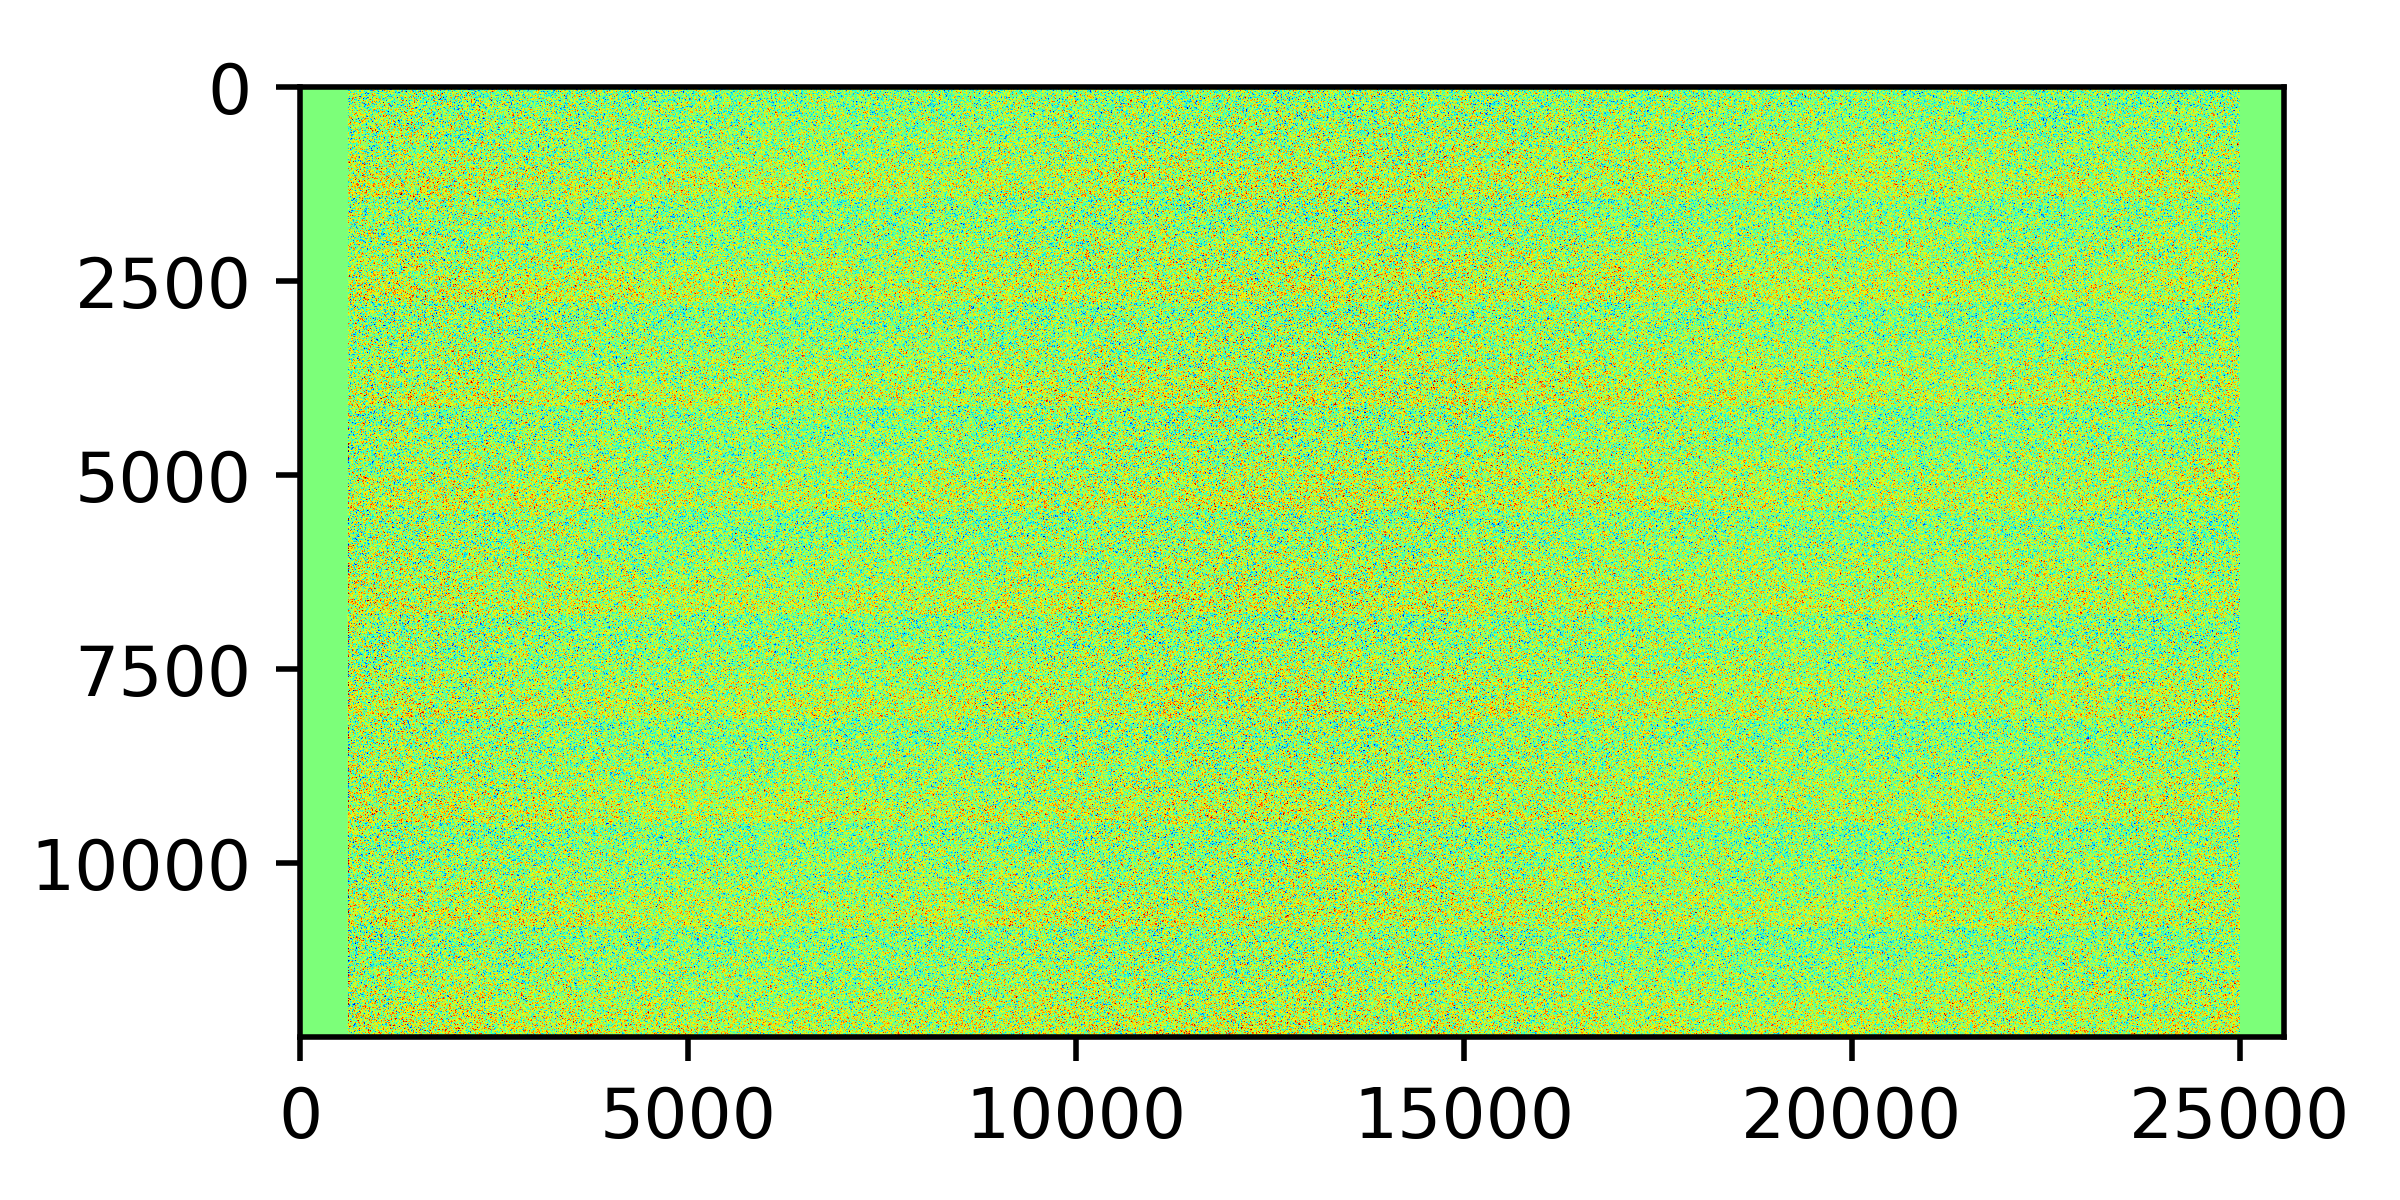
\includegraphics[width=\textwidth]{figure/The cross-interferogram/cross_interf_TaklimakanDesert_asc.png}
        \end{minipage}%
        \begin{minipage}[c]{0.5\textwidth}
            \centering
            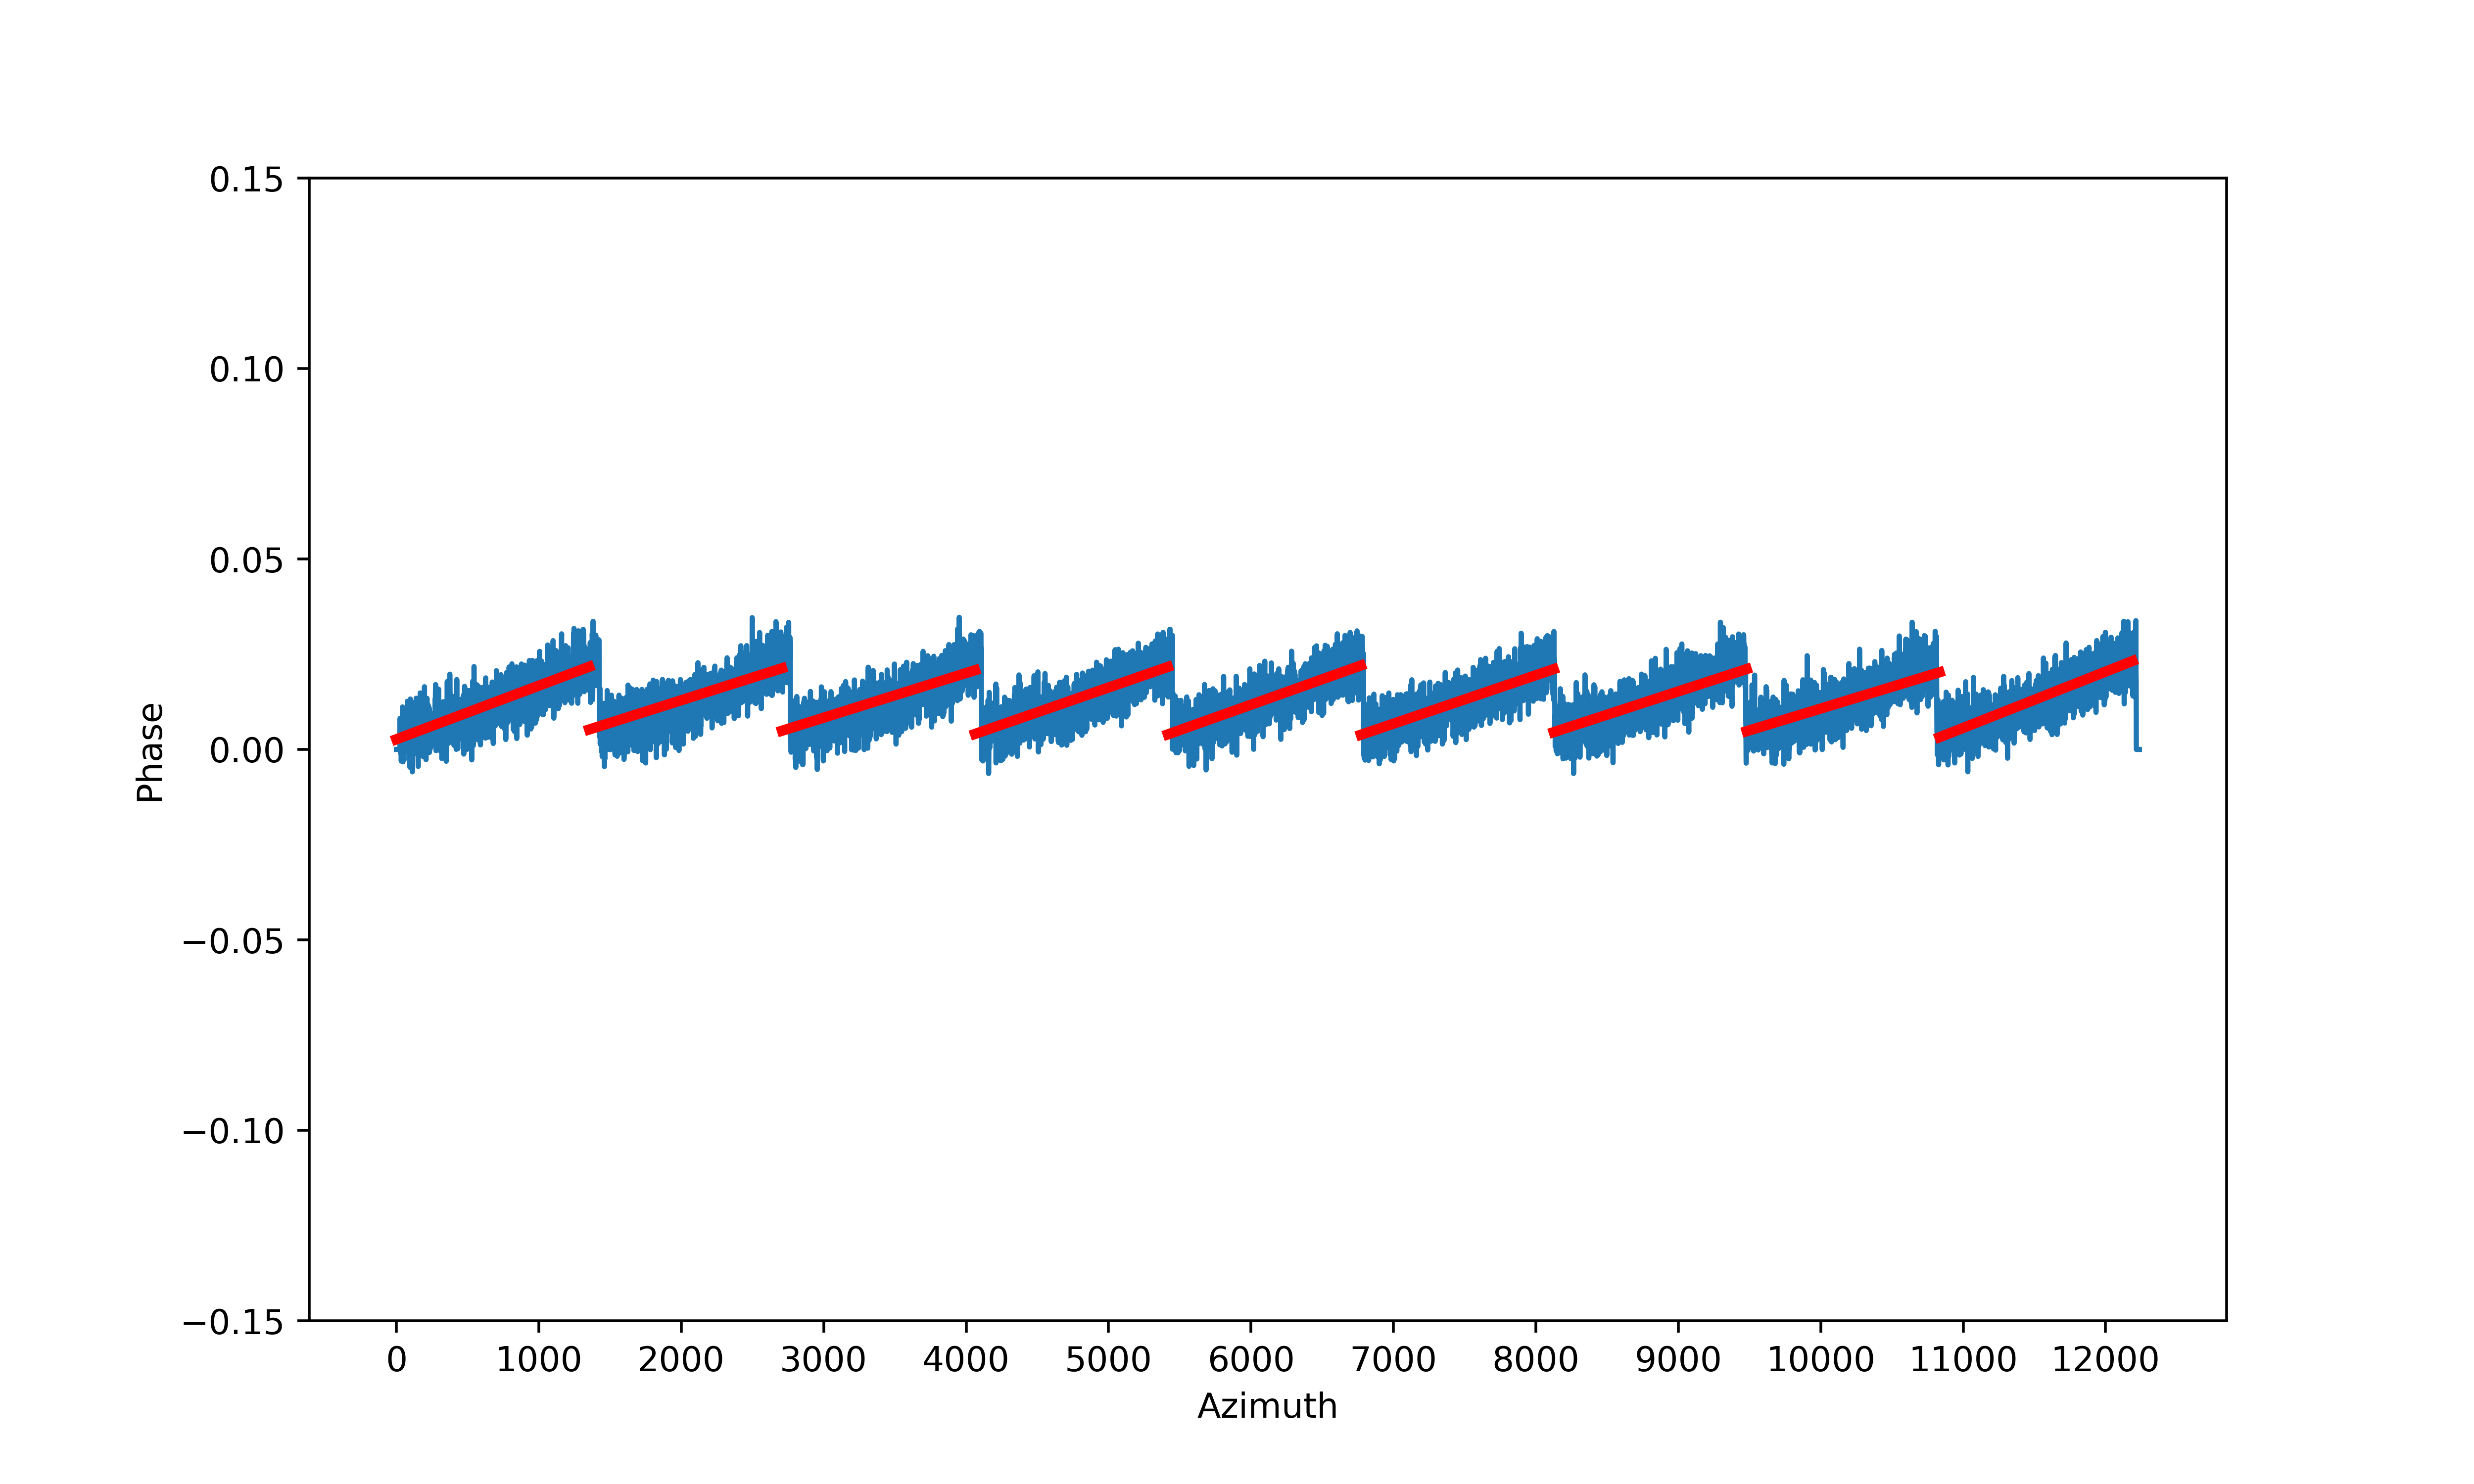
\includegraphics[width=\textwidth]{figure/The cross-interferogram/cross_interf_TaklimakanDesert_asc_row&fitted_20230102.png}
        \end{minipage}
        \caption{Taklamakan desert ascending}
        \label{fig_5a}
    \end{subfigure}%
    \begin{subfigure}[c]{0.5\textwidth}
        \centering
        \begin{minipage}[c]{0.5\textwidth}
            \centering
            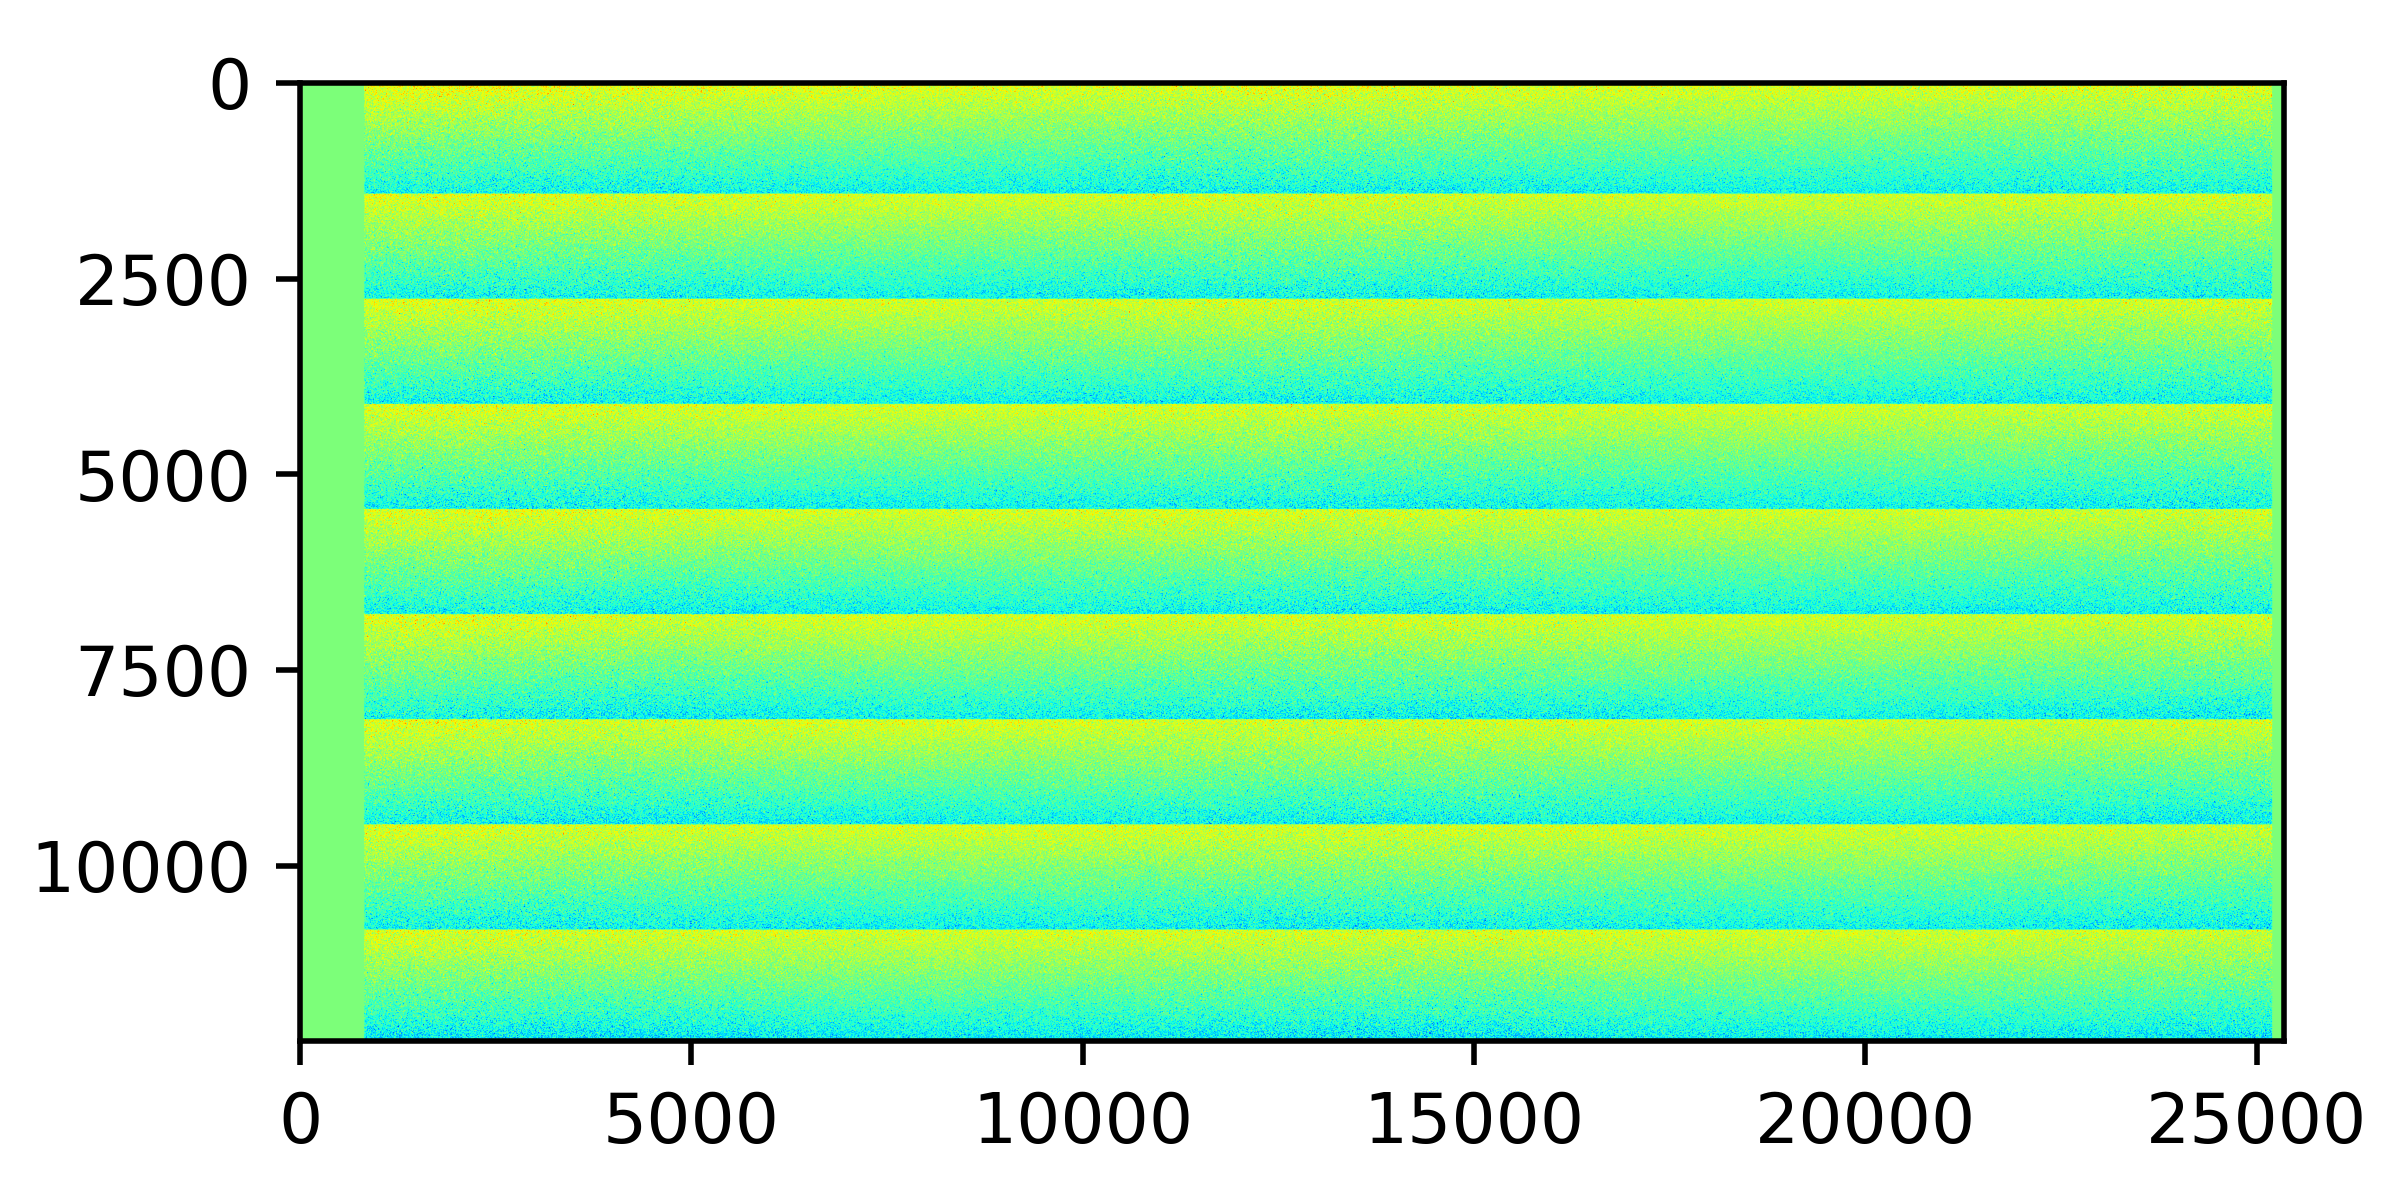
\includegraphics[width=\textwidth]{figure/The cross-interferogram/cross_interf_TaklimakanDesert_des.png}
        \end{minipage}%
        \begin{minipage}[c]{0.5\textwidth}
            \centering
            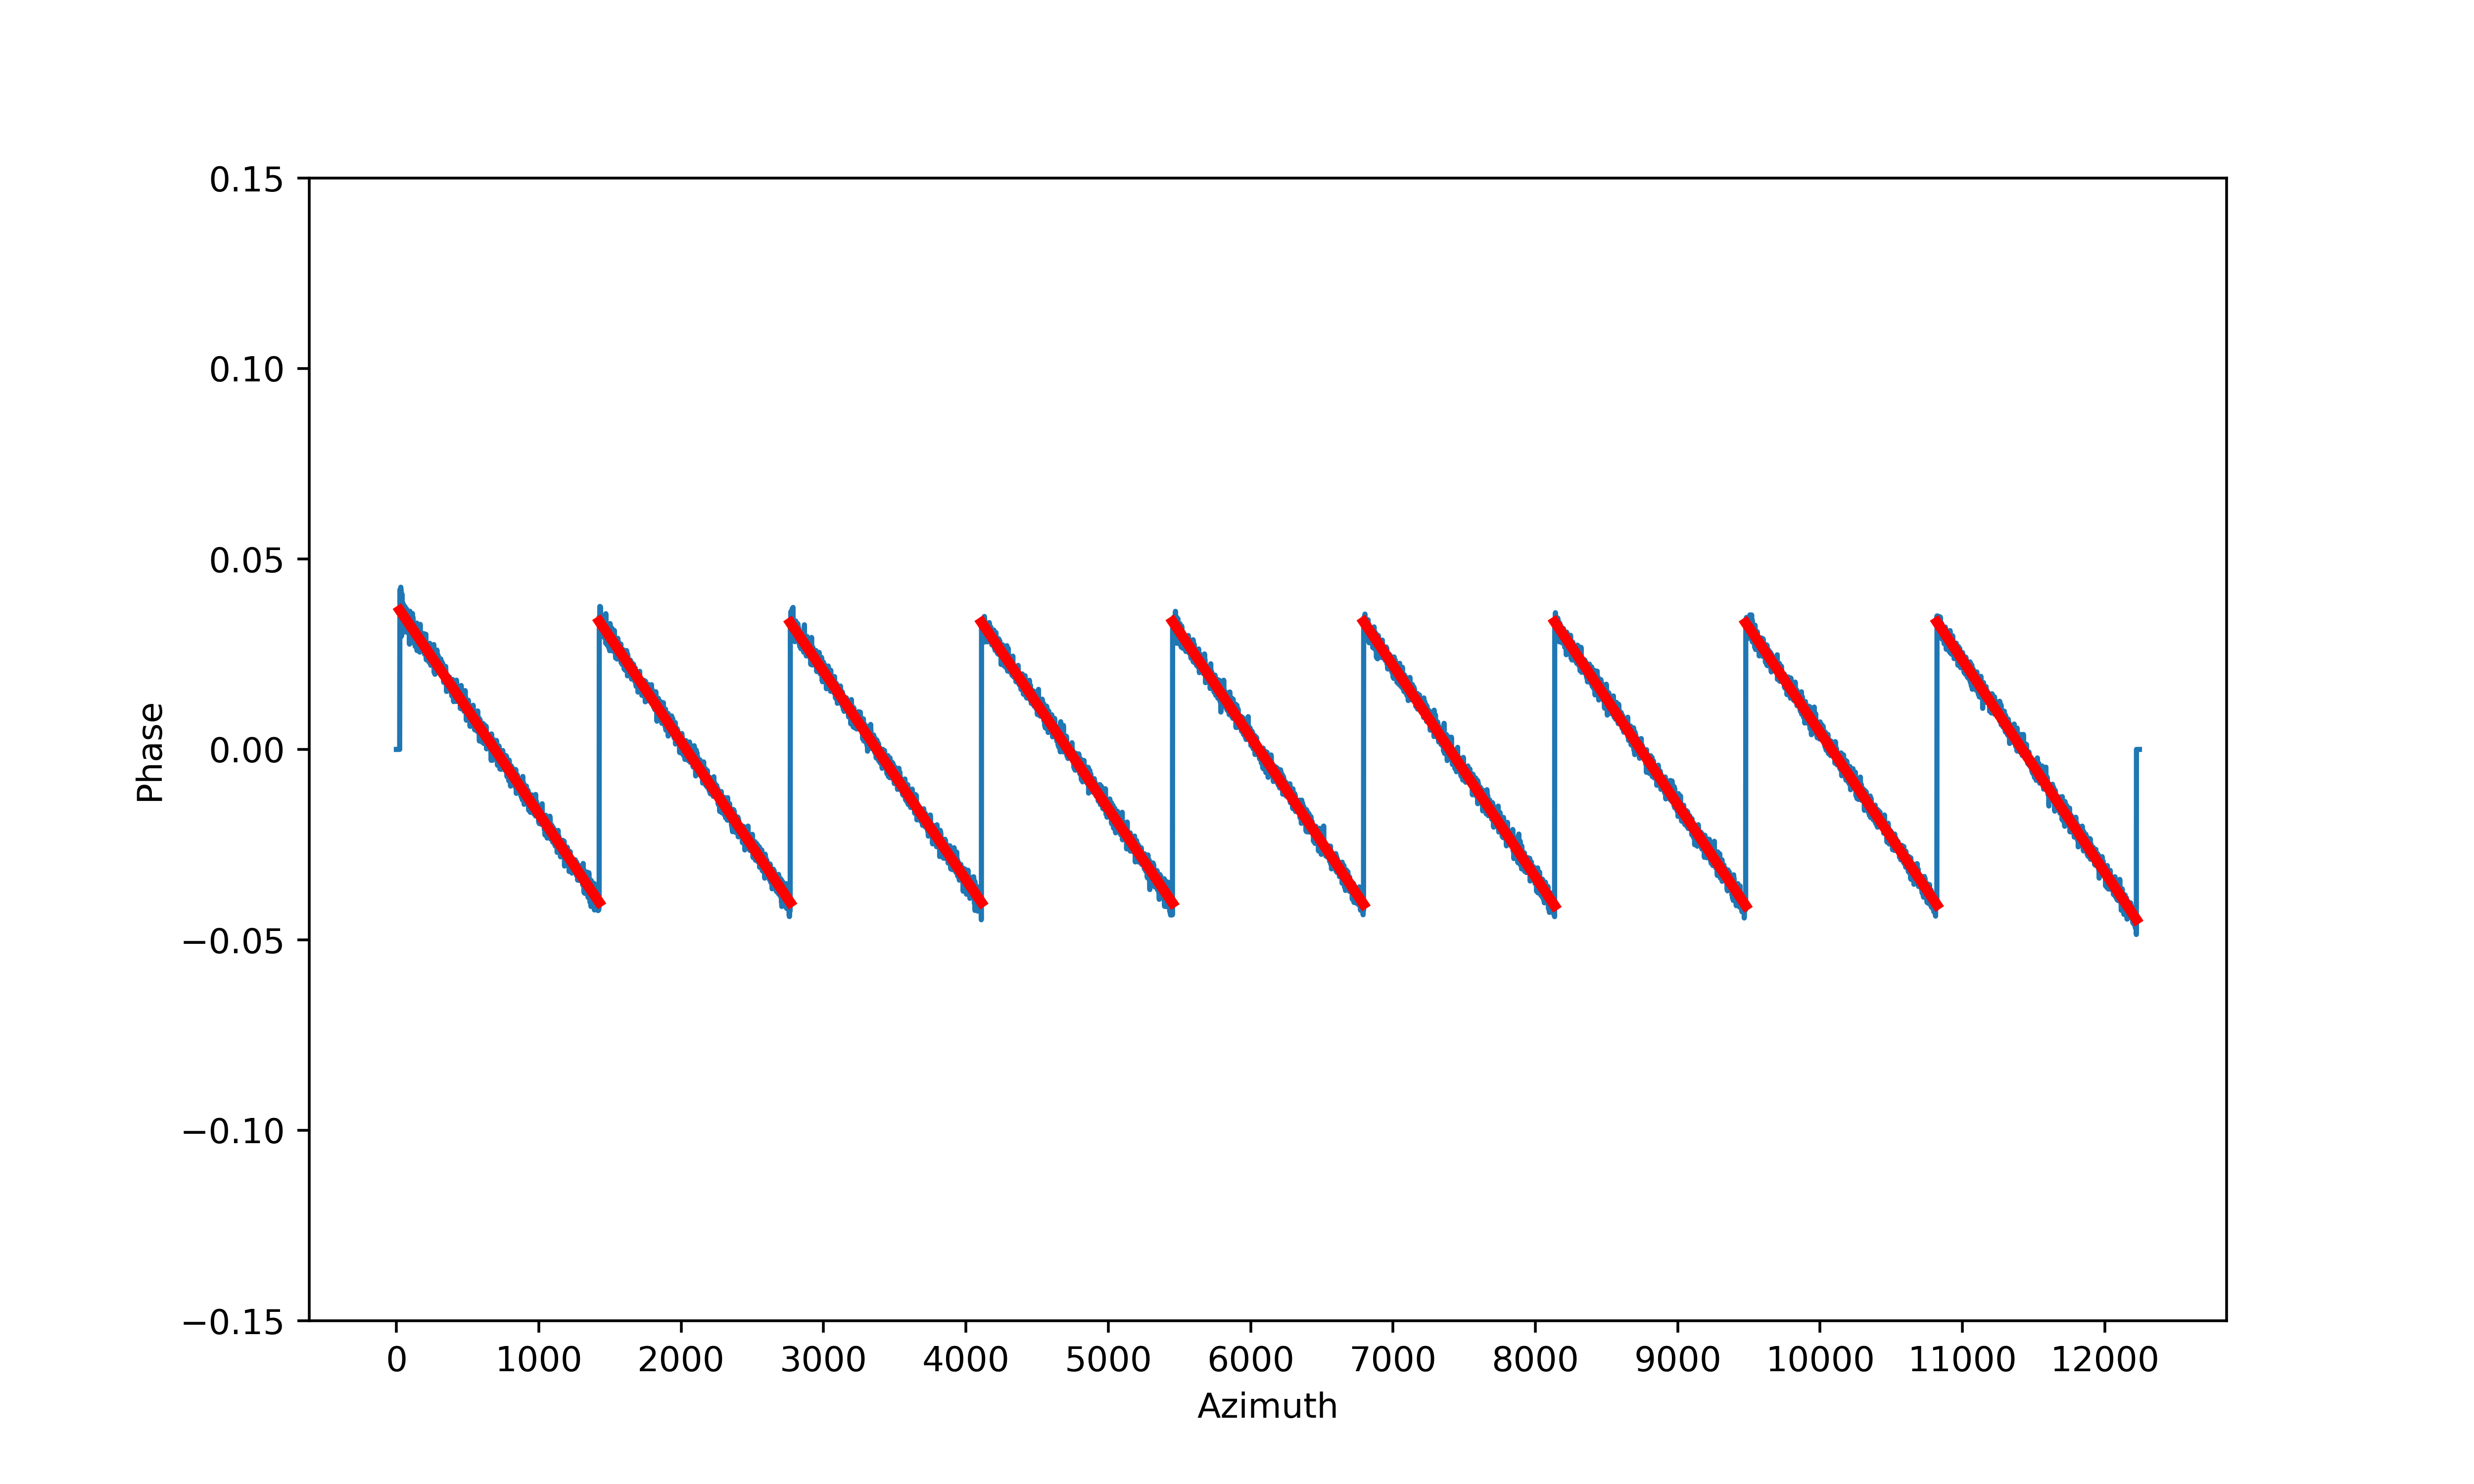
\includegraphics[width=\textwidth]{figure/The cross-interferogram/cross_interf_TaklimakanDesert_des_row&fitted_20230108.png}
        \end{minipage}
        \caption{Taklamakan desert descending}
        \label{fig_5b}
    \end{subfigure}%
    \hfill
    \begin{subfigure}{0.5\textwidth}
        \centering
        \begin{minipage}{0.5\textwidth}
            \centering
            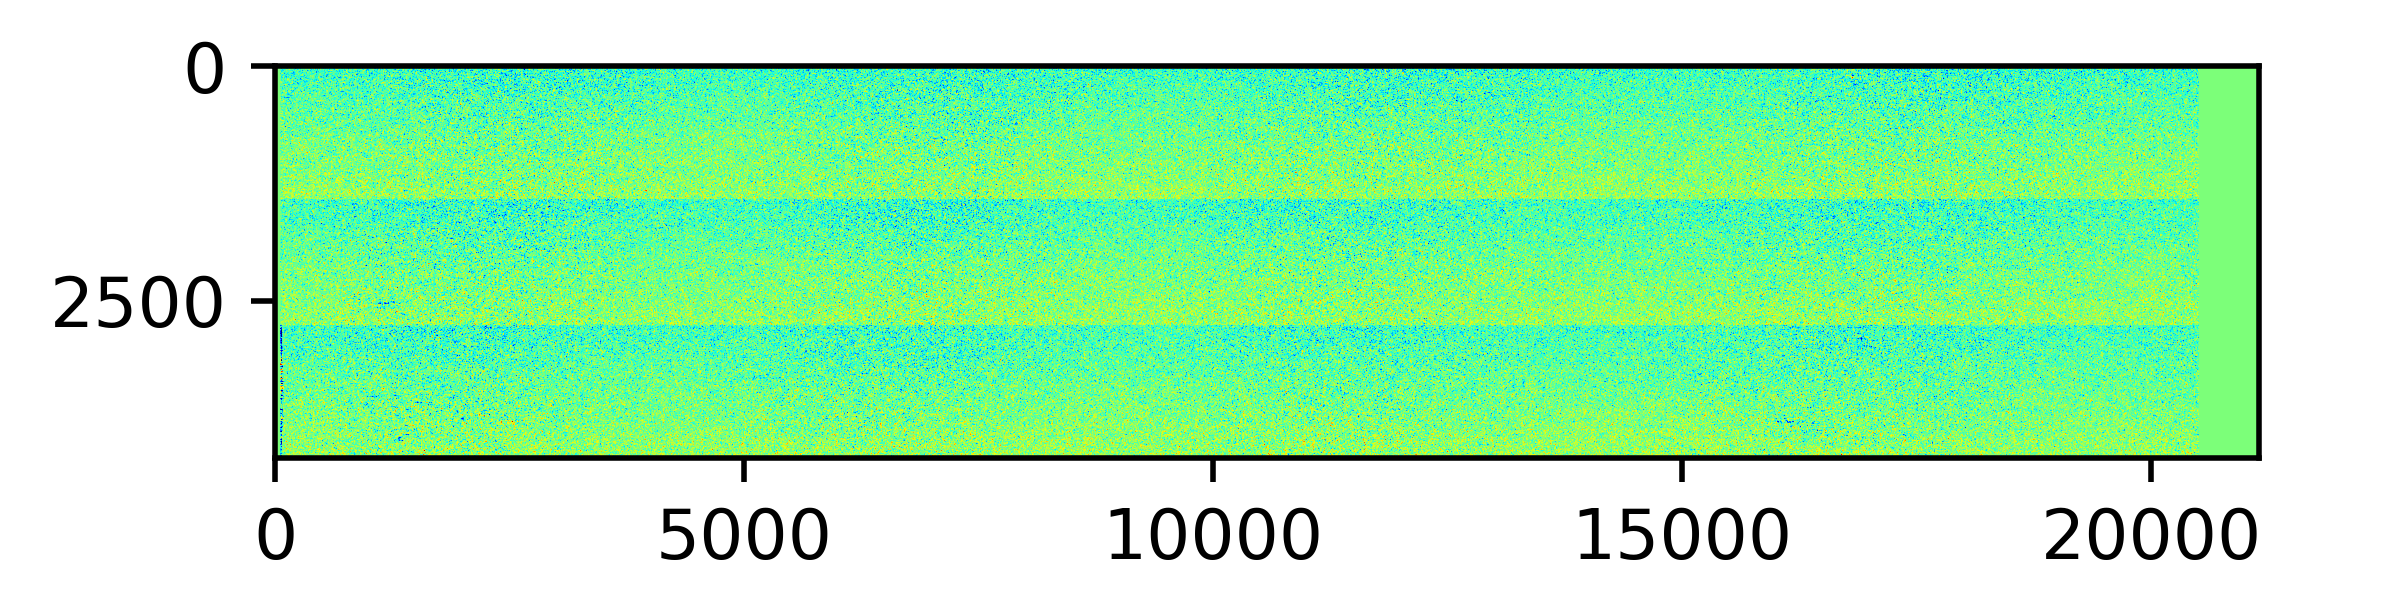
\includegraphics[width=\textwidth]{figure/The cross-interferogram/cross_interf_Mexico_asc.png}
        \end{minipage}%
        \begin{minipage}{0.5\textwidth}
            \centering
            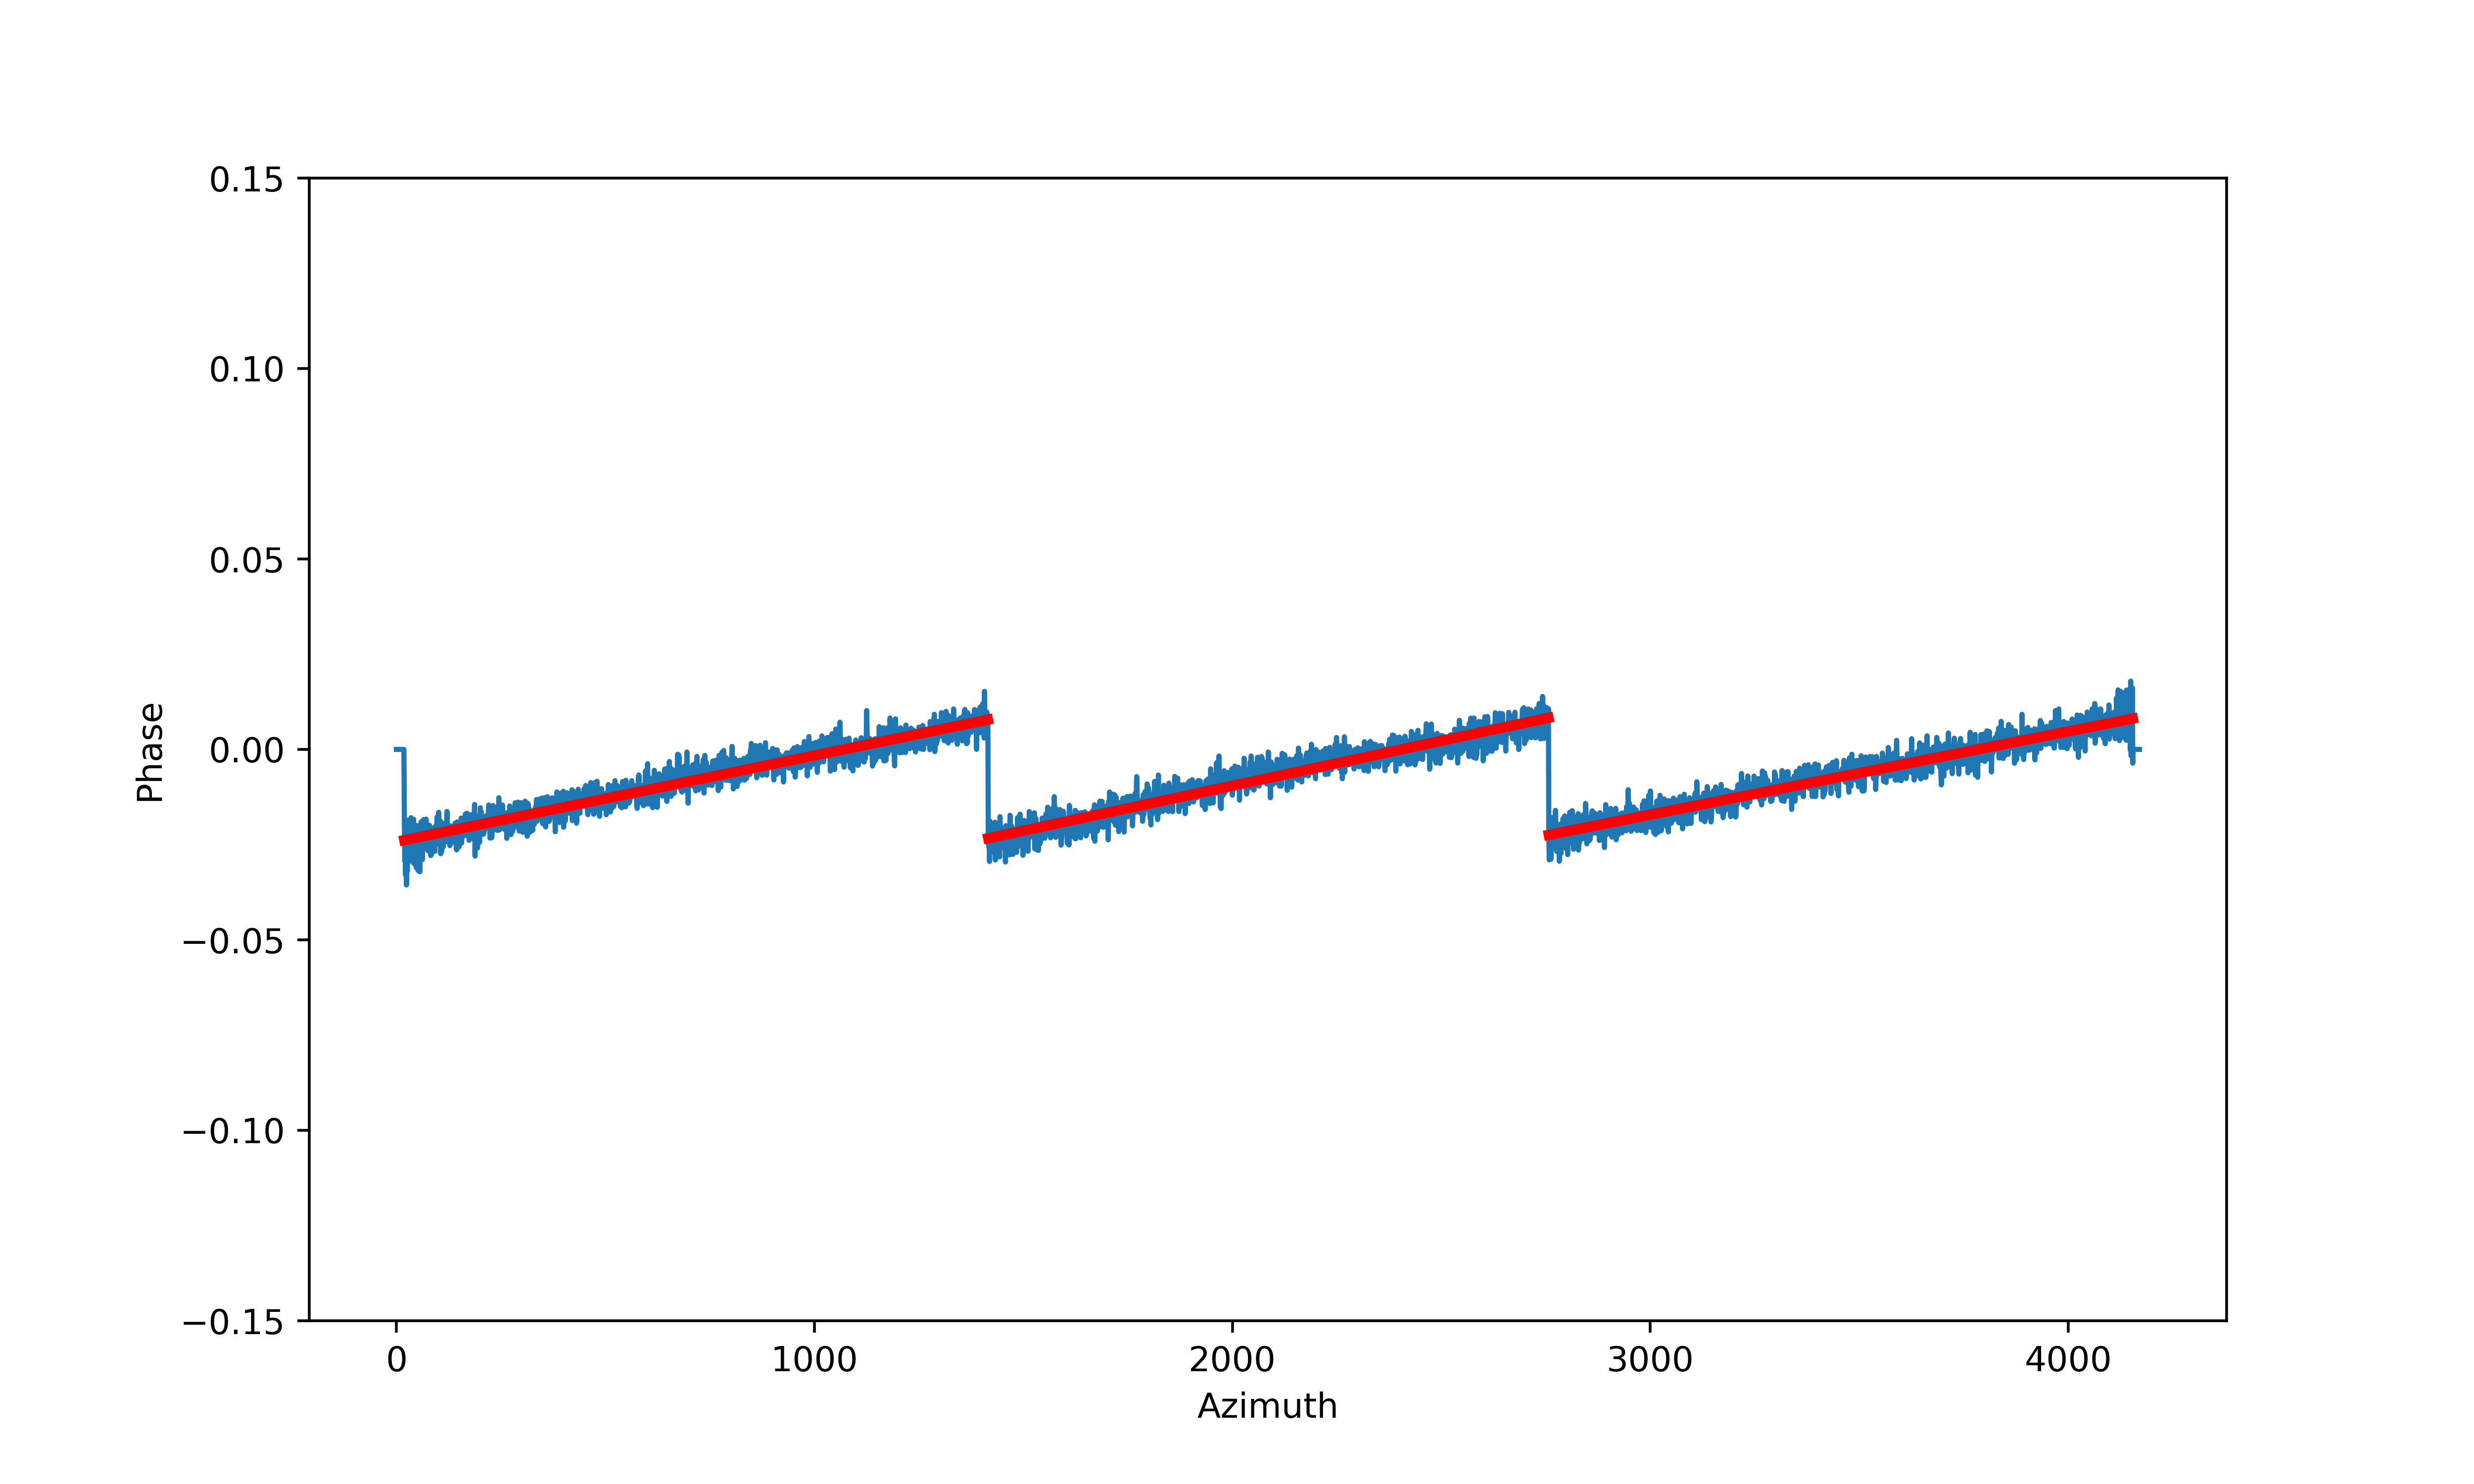
\includegraphics[width=\textwidth]{figure/The cross-interferogram/cross_interf_Mexico_asc_row&fitted_20230104.png}
        \end{minipage}
        \caption{Mexico City ascending}
        \label{fig_5c}
    \end{subfigure}%
    \begin{subfigure}{0.5\textwidth}
        \centering
        \begin{minipage}{0.5\textwidth}
            \centering
            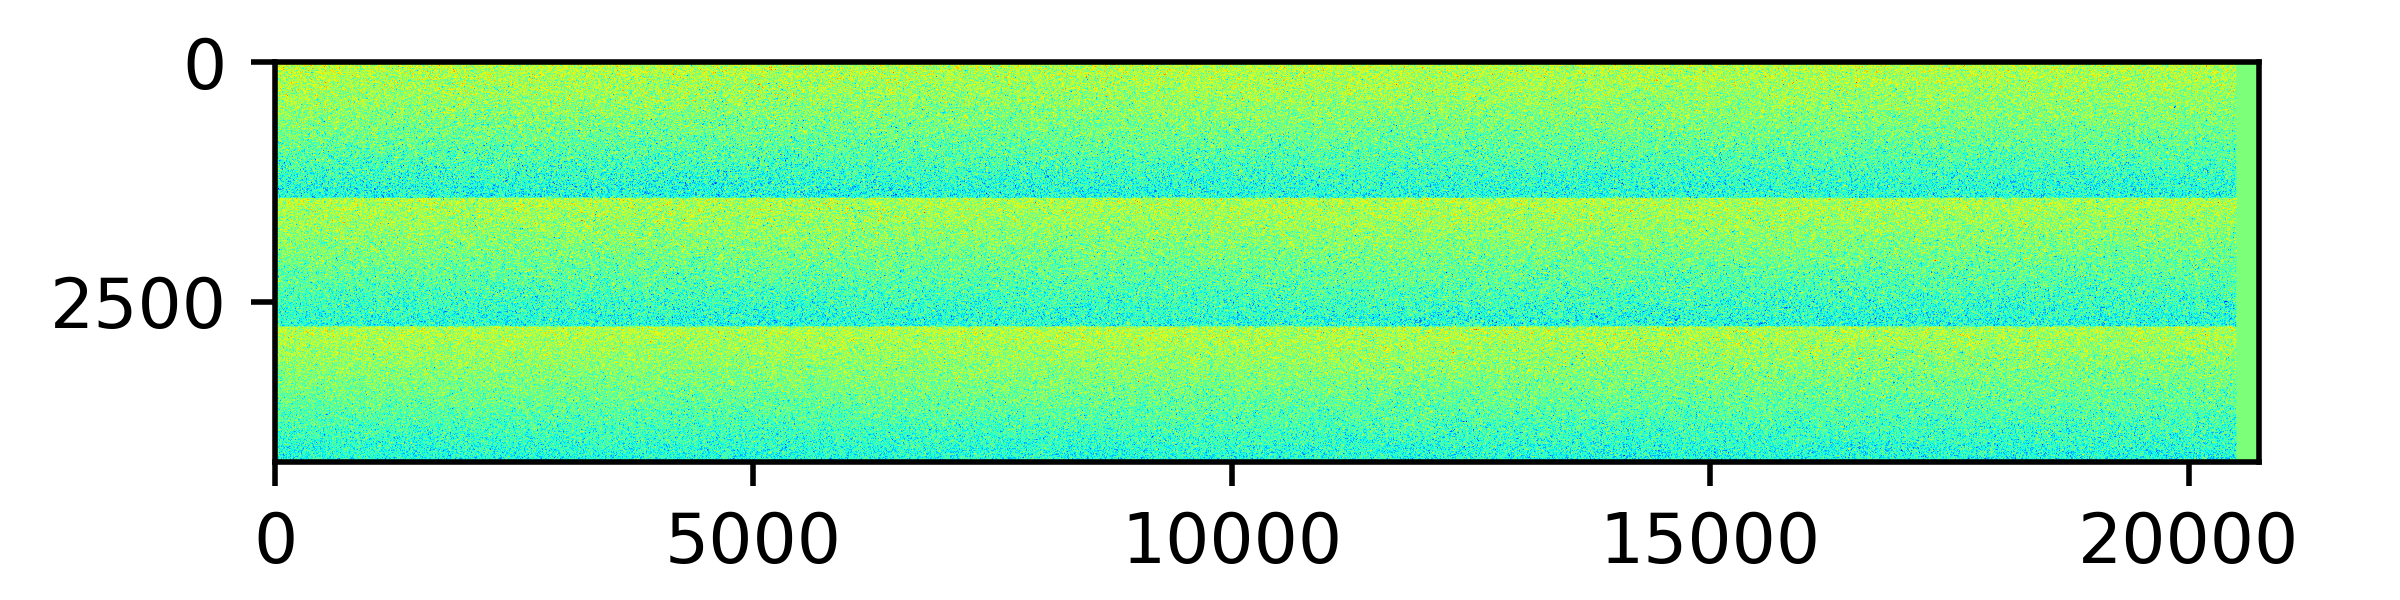
\includegraphics[width=\textwidth]{figure/The cross-interferogram/cross_interf_Mexico_des.png}
        \end{minipage}%
        \begin{minipage}{0.5\textwidth}
            \centering
            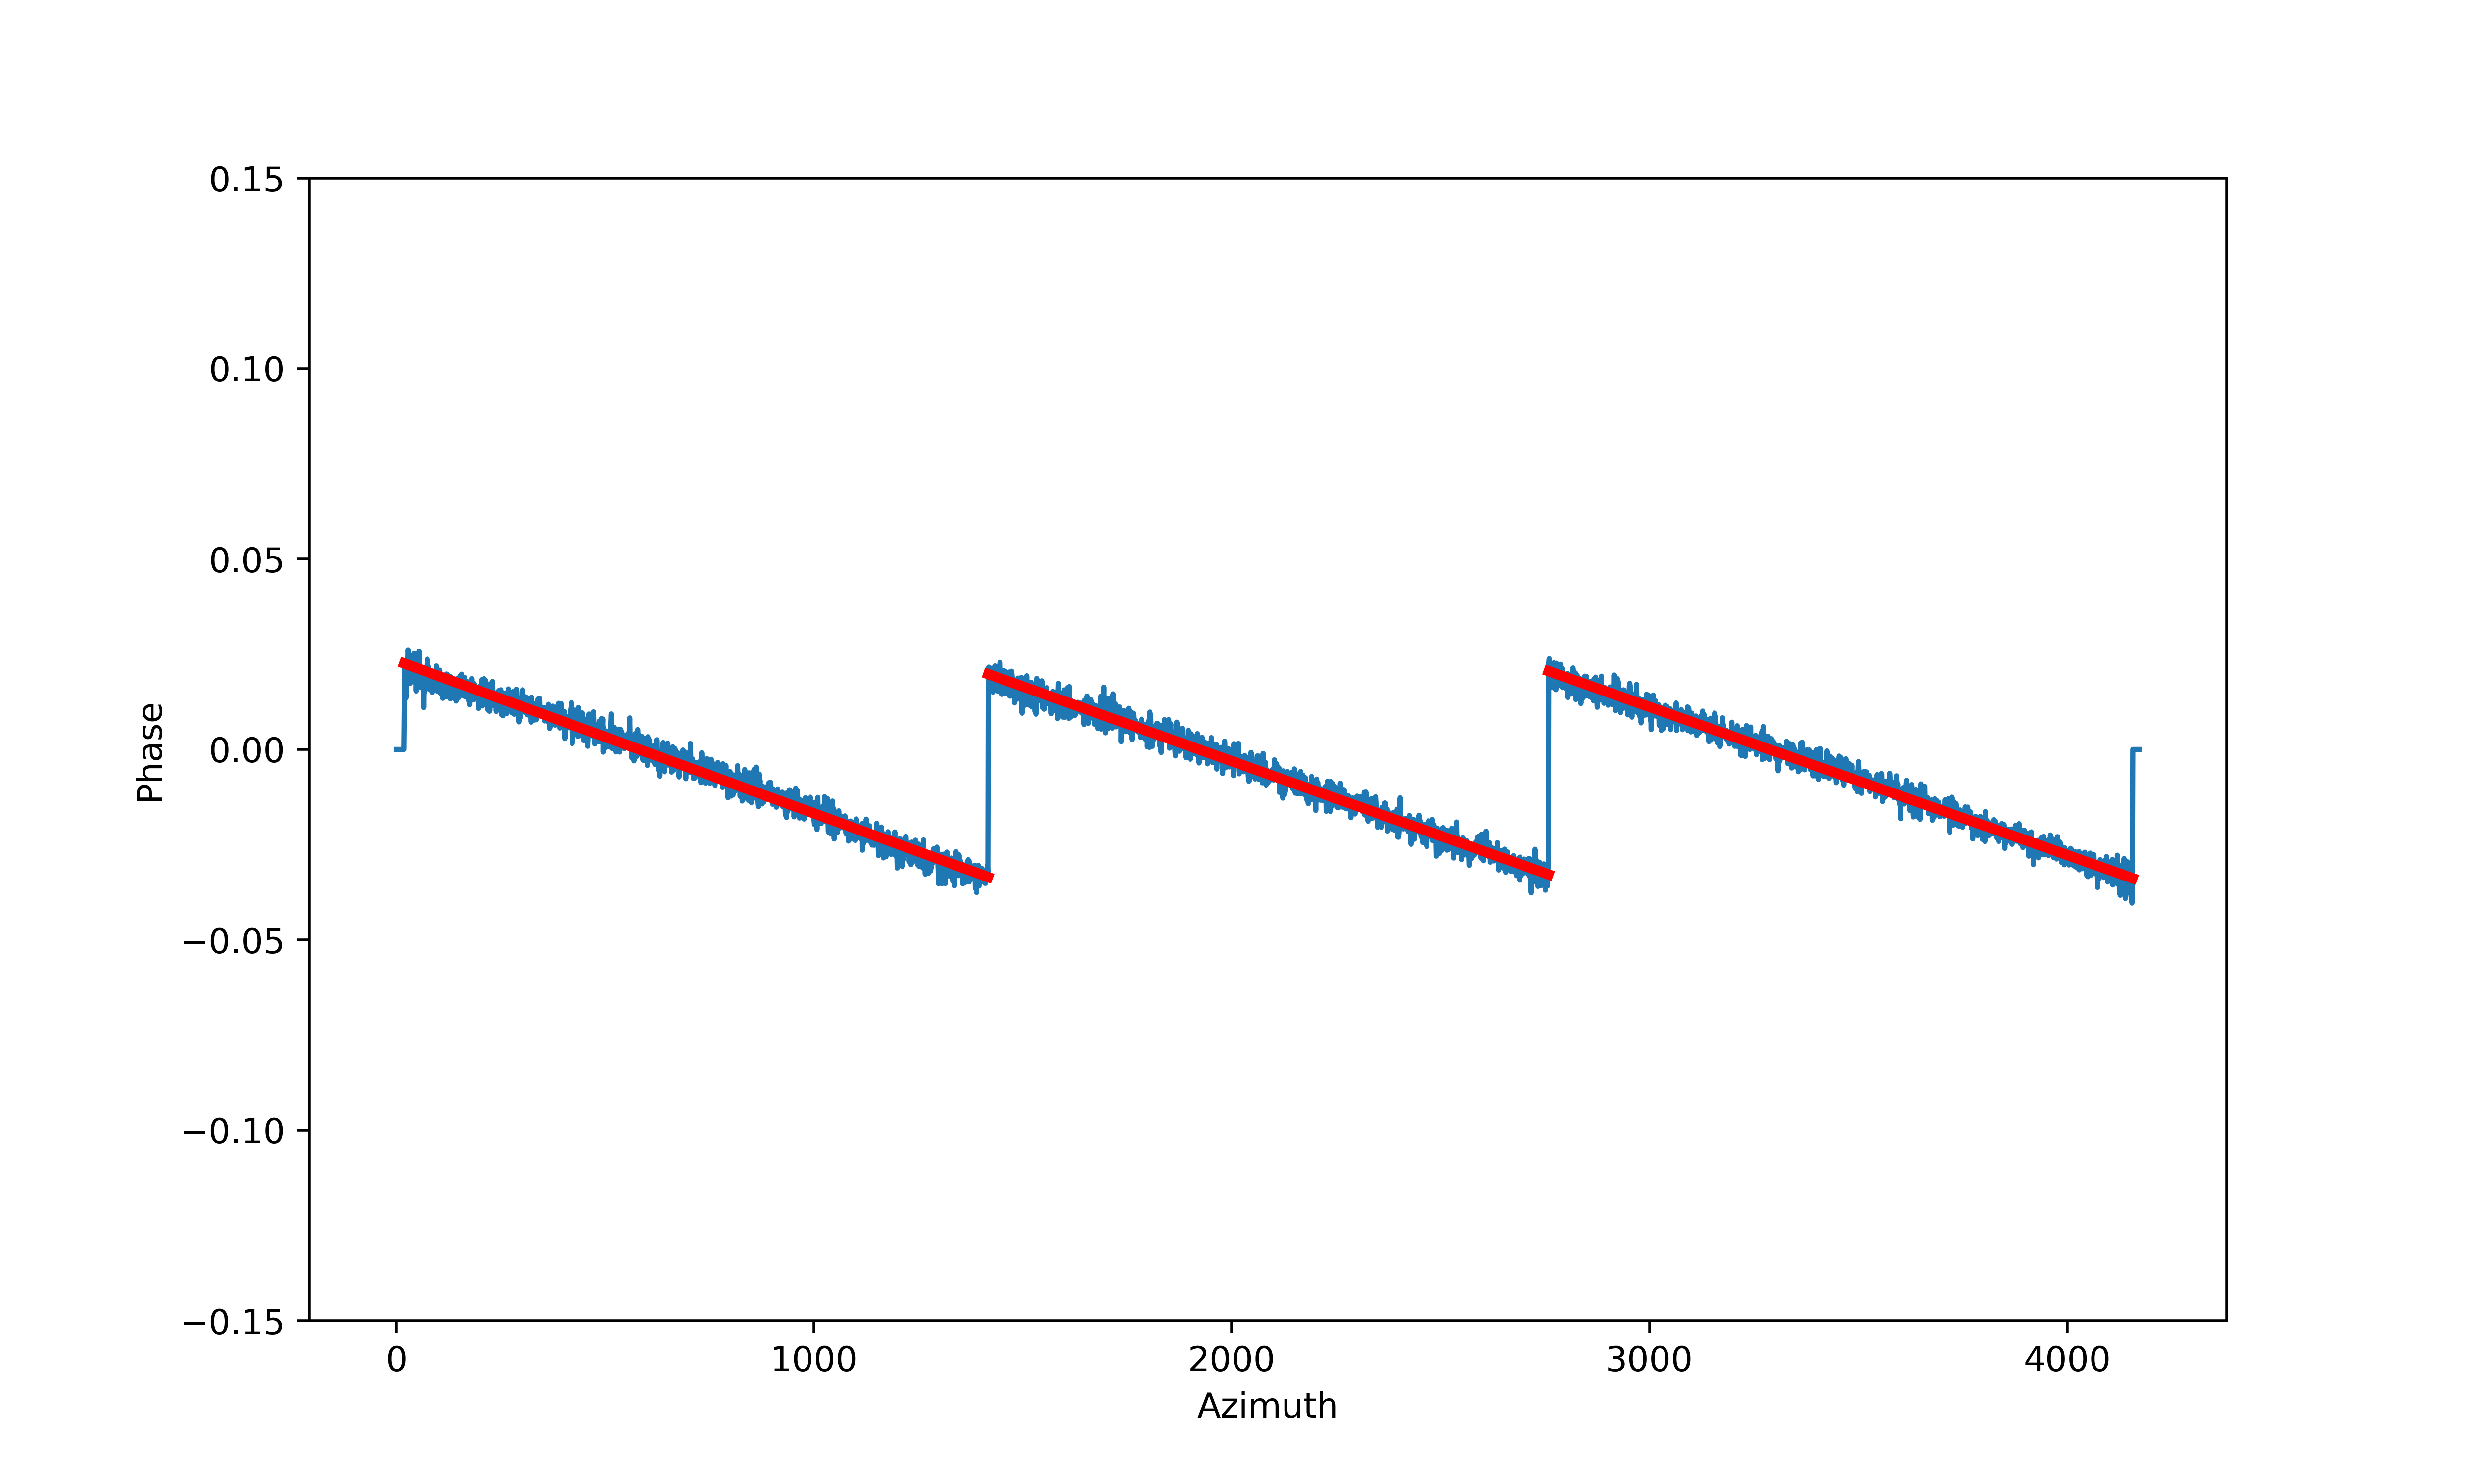
\includegraphics[width=\textwidth]{figure/The cross-interferogram/cross_interf_Mexico_des_row&fitted_20230106.png}
        \end{minipage}
        \caption{Mexico City descending}
        \label{fig_5d}
    \end{subfigure}%
    \hfill
    \begin{subfigure}{0.5\textwidth}
        \centering
        \begin{minipage}{0.5\textwidth}
            \centering
            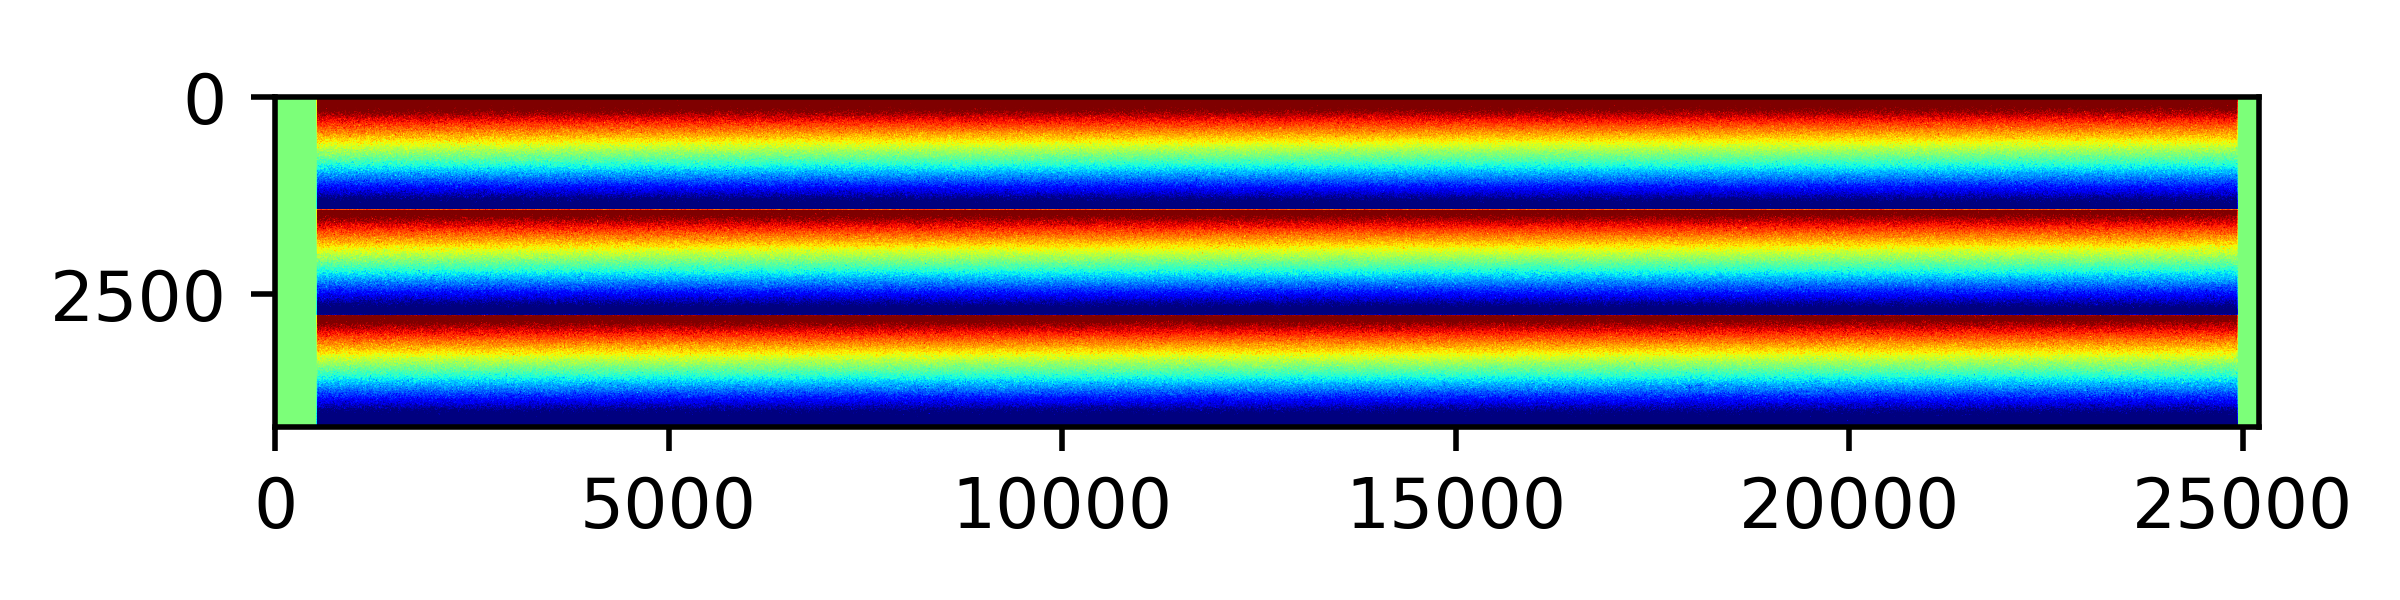
\includegraphics[width=\textwidth]{figure/The cross-interferogram/cross_interf_XiAn_asc.png}
        \end{minipage}%
        \begin{minipage}{0.5\textwidth}
            \centering
            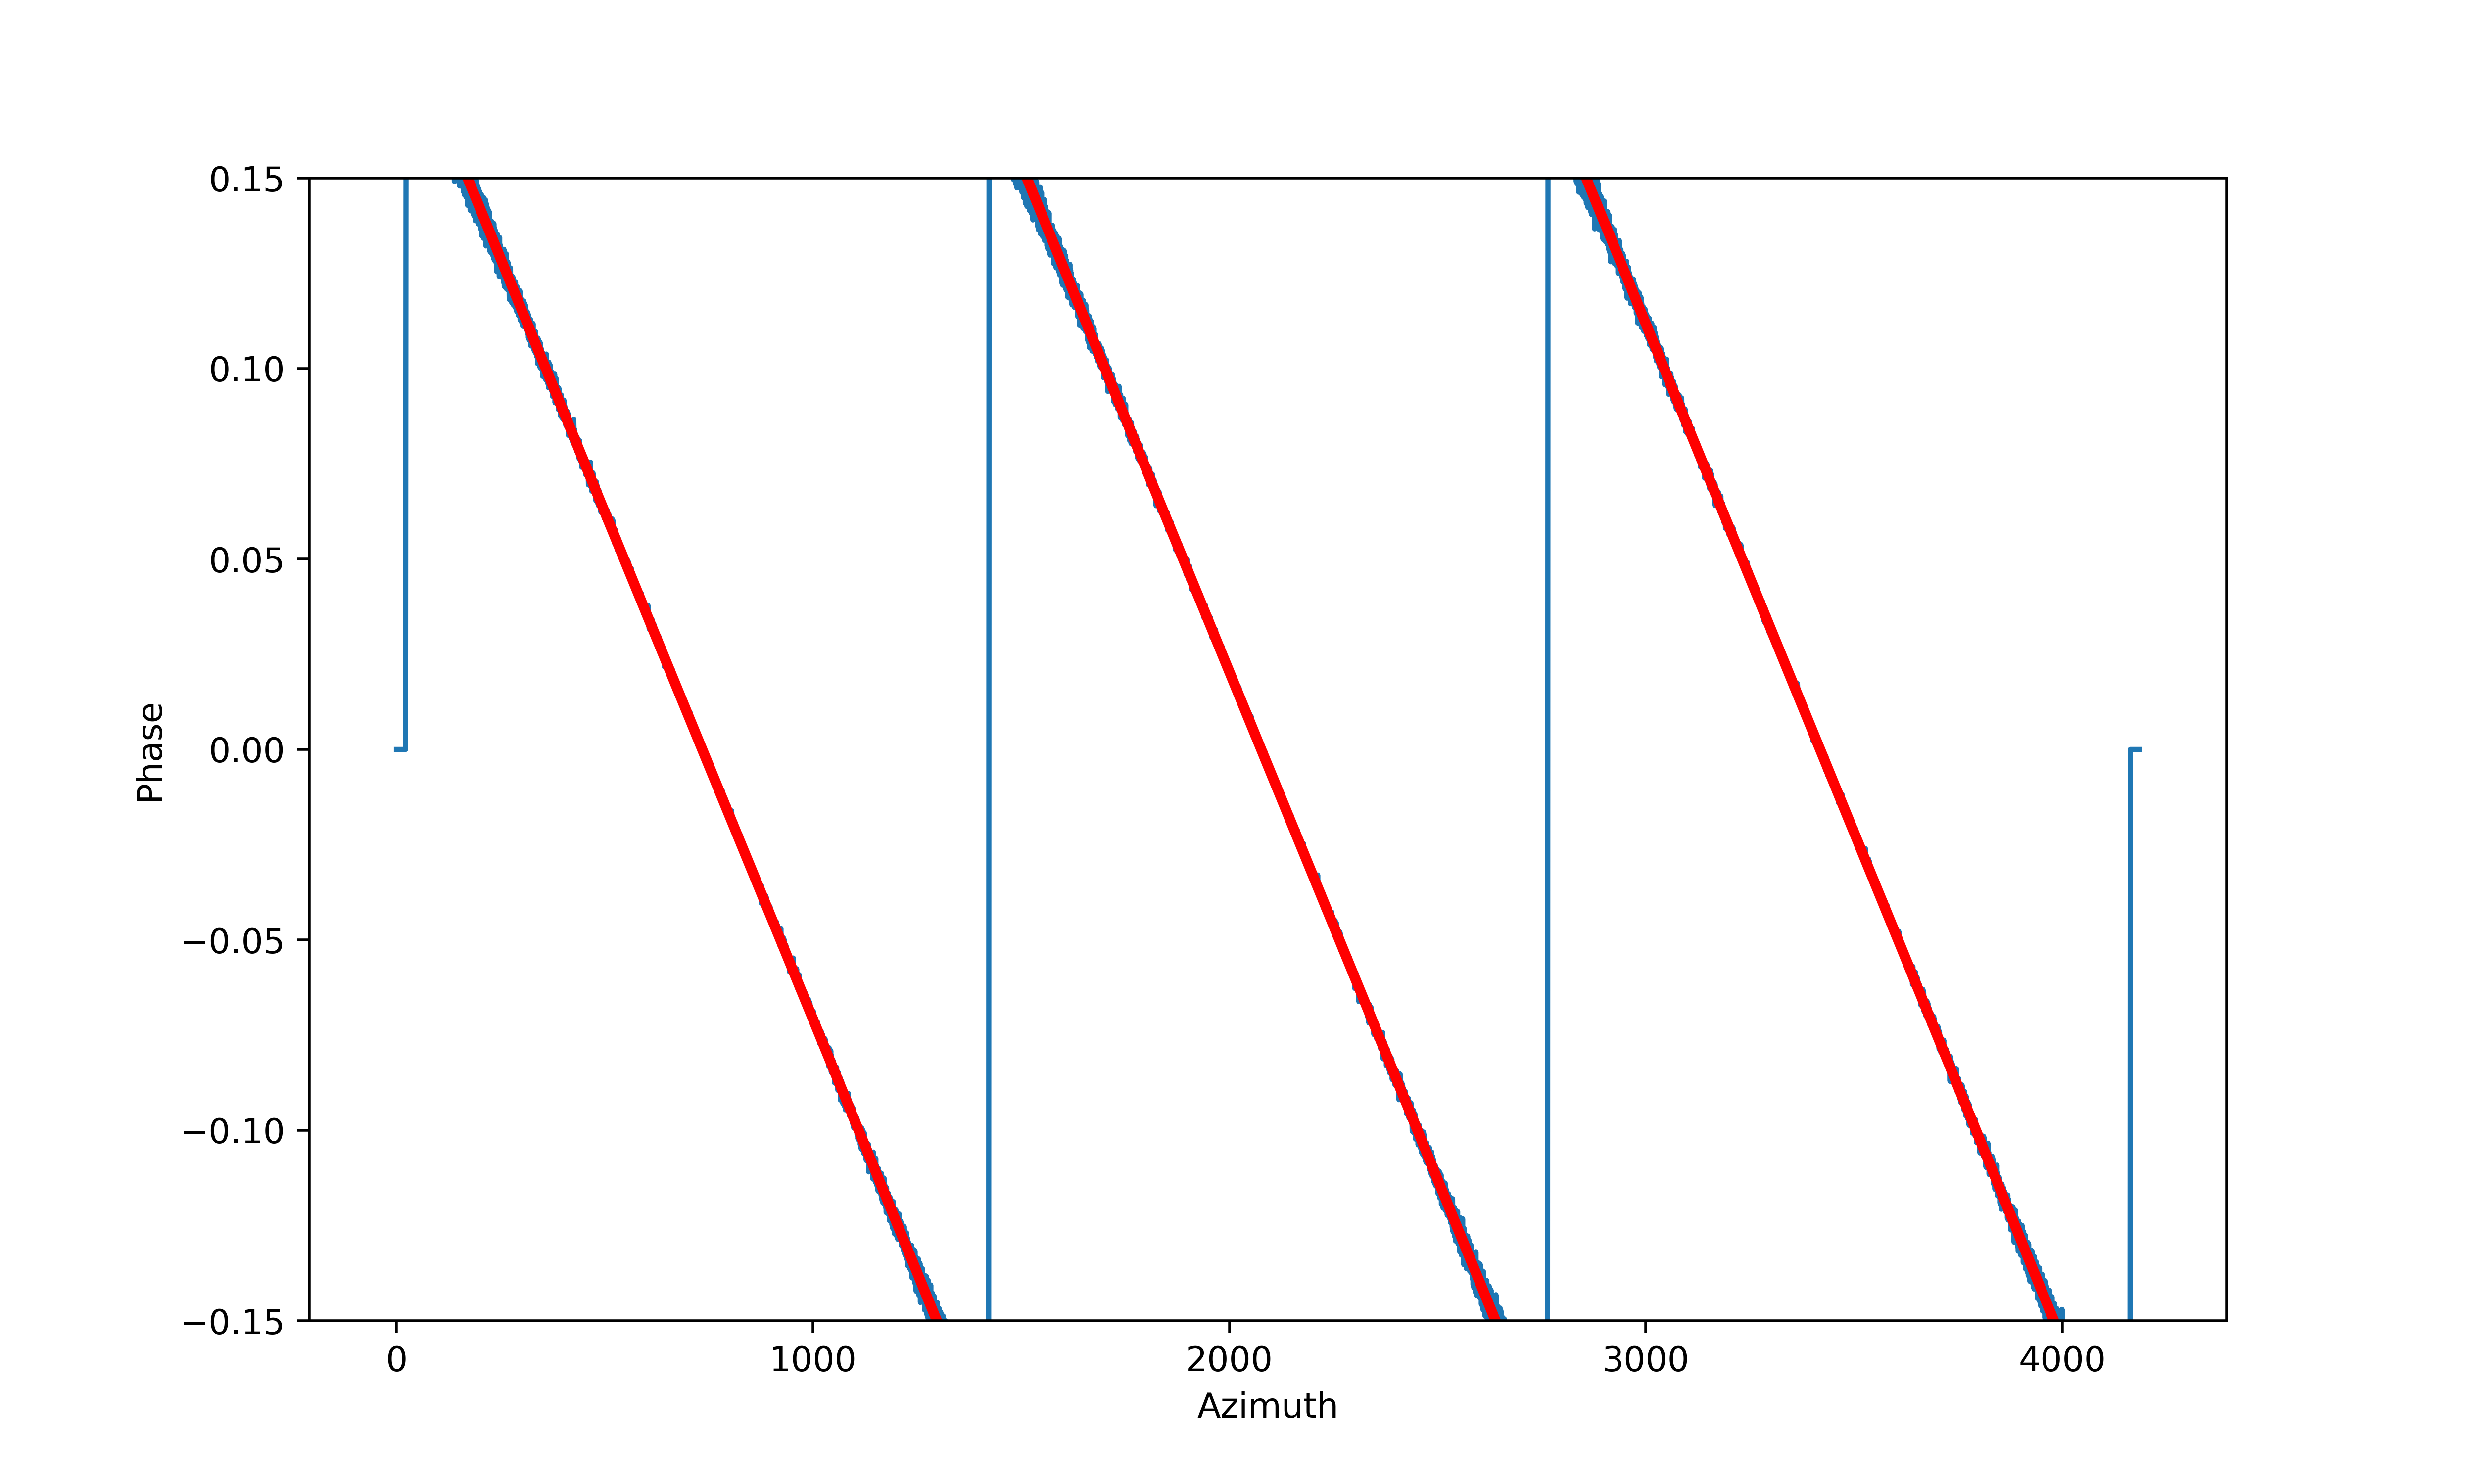
\includegraphics[width=\textwidth]{figure/The cross-interferogram/cross_interf_XiAn_asc_row&fitted_20230109.png}
        \end{minipage}
        \caption{Xi'an ascending}
        \label{fig_5e}
    \end{subfigure}%
    \begin{subfigure}{0.5\textwidth}
        \centering
        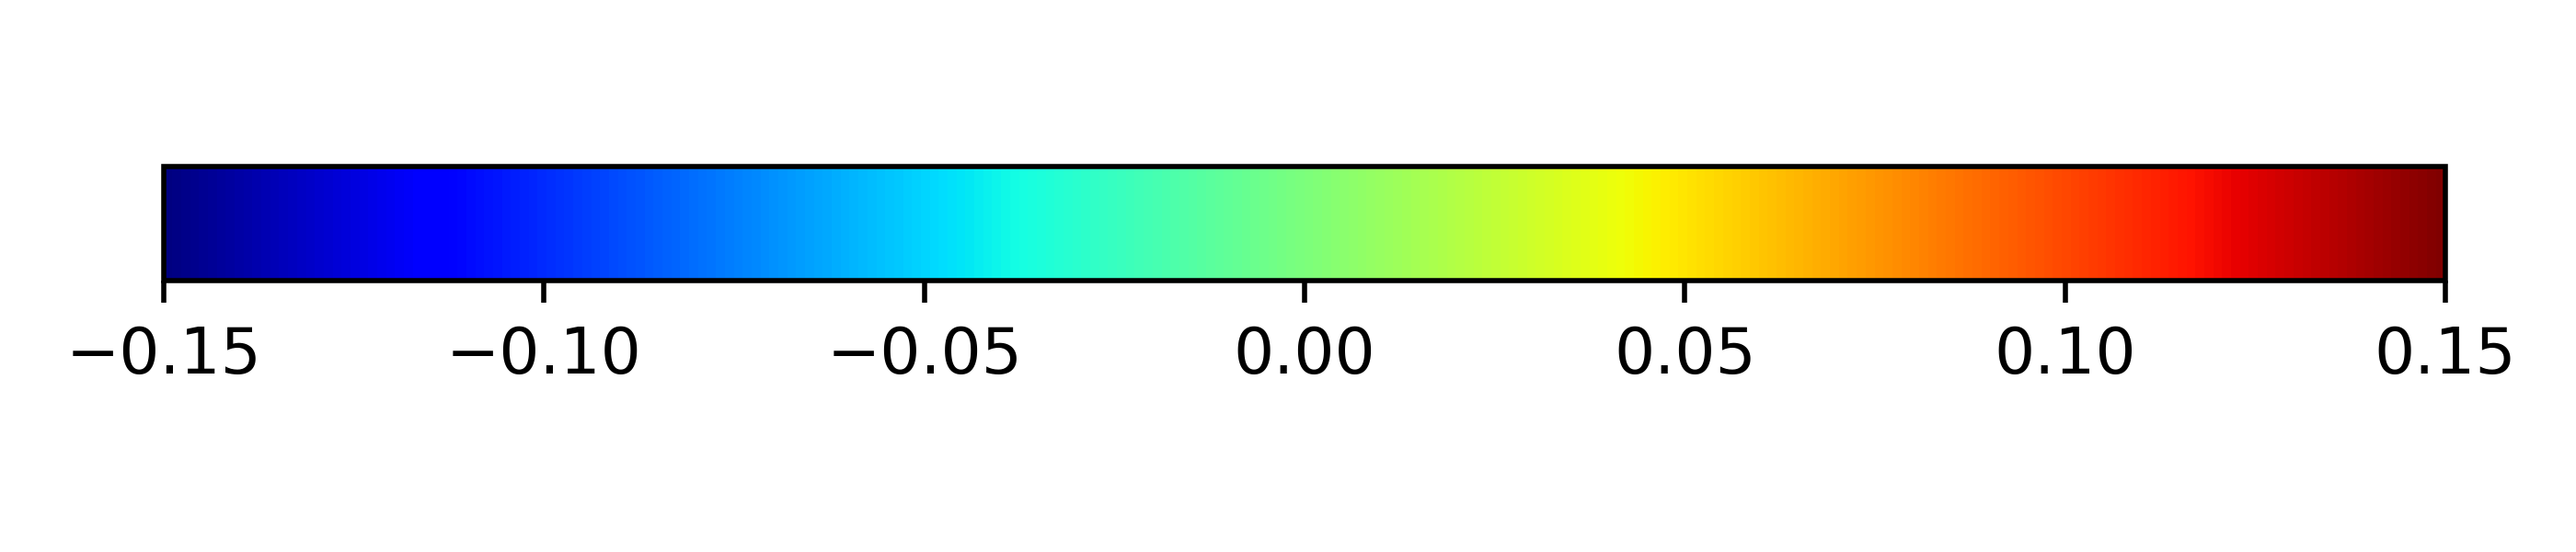
\includegraphics[width=\textwidth]{figure/The cross-interferogram/colorbar.png}
        \caption*{}
    \end{subfigure}%
    \hfill
    \begin{subfigure}{0.5\textwidth}
        \centering
        \begin{minipage}{0.5\textwidth}
            \centering
            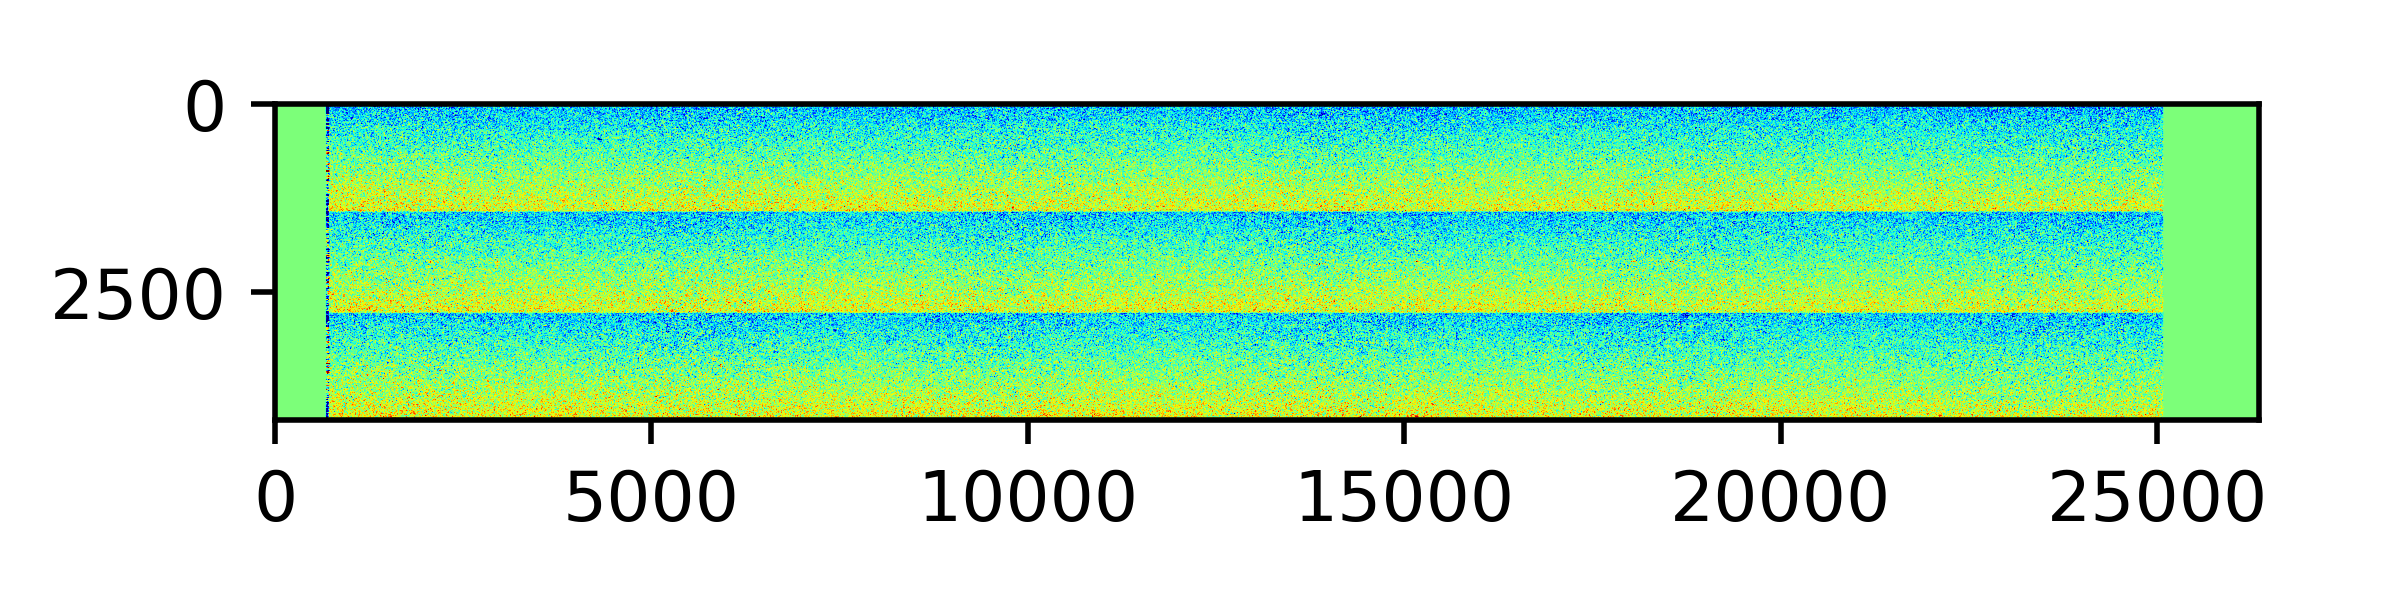
\includegraphics[width=\textwidth]{figure/The cross-interferogram/cross_interf_Milan_asc.png}
        \end{minipage}%
        \begin{minipage}{0.5\textwidth}
            \centering
            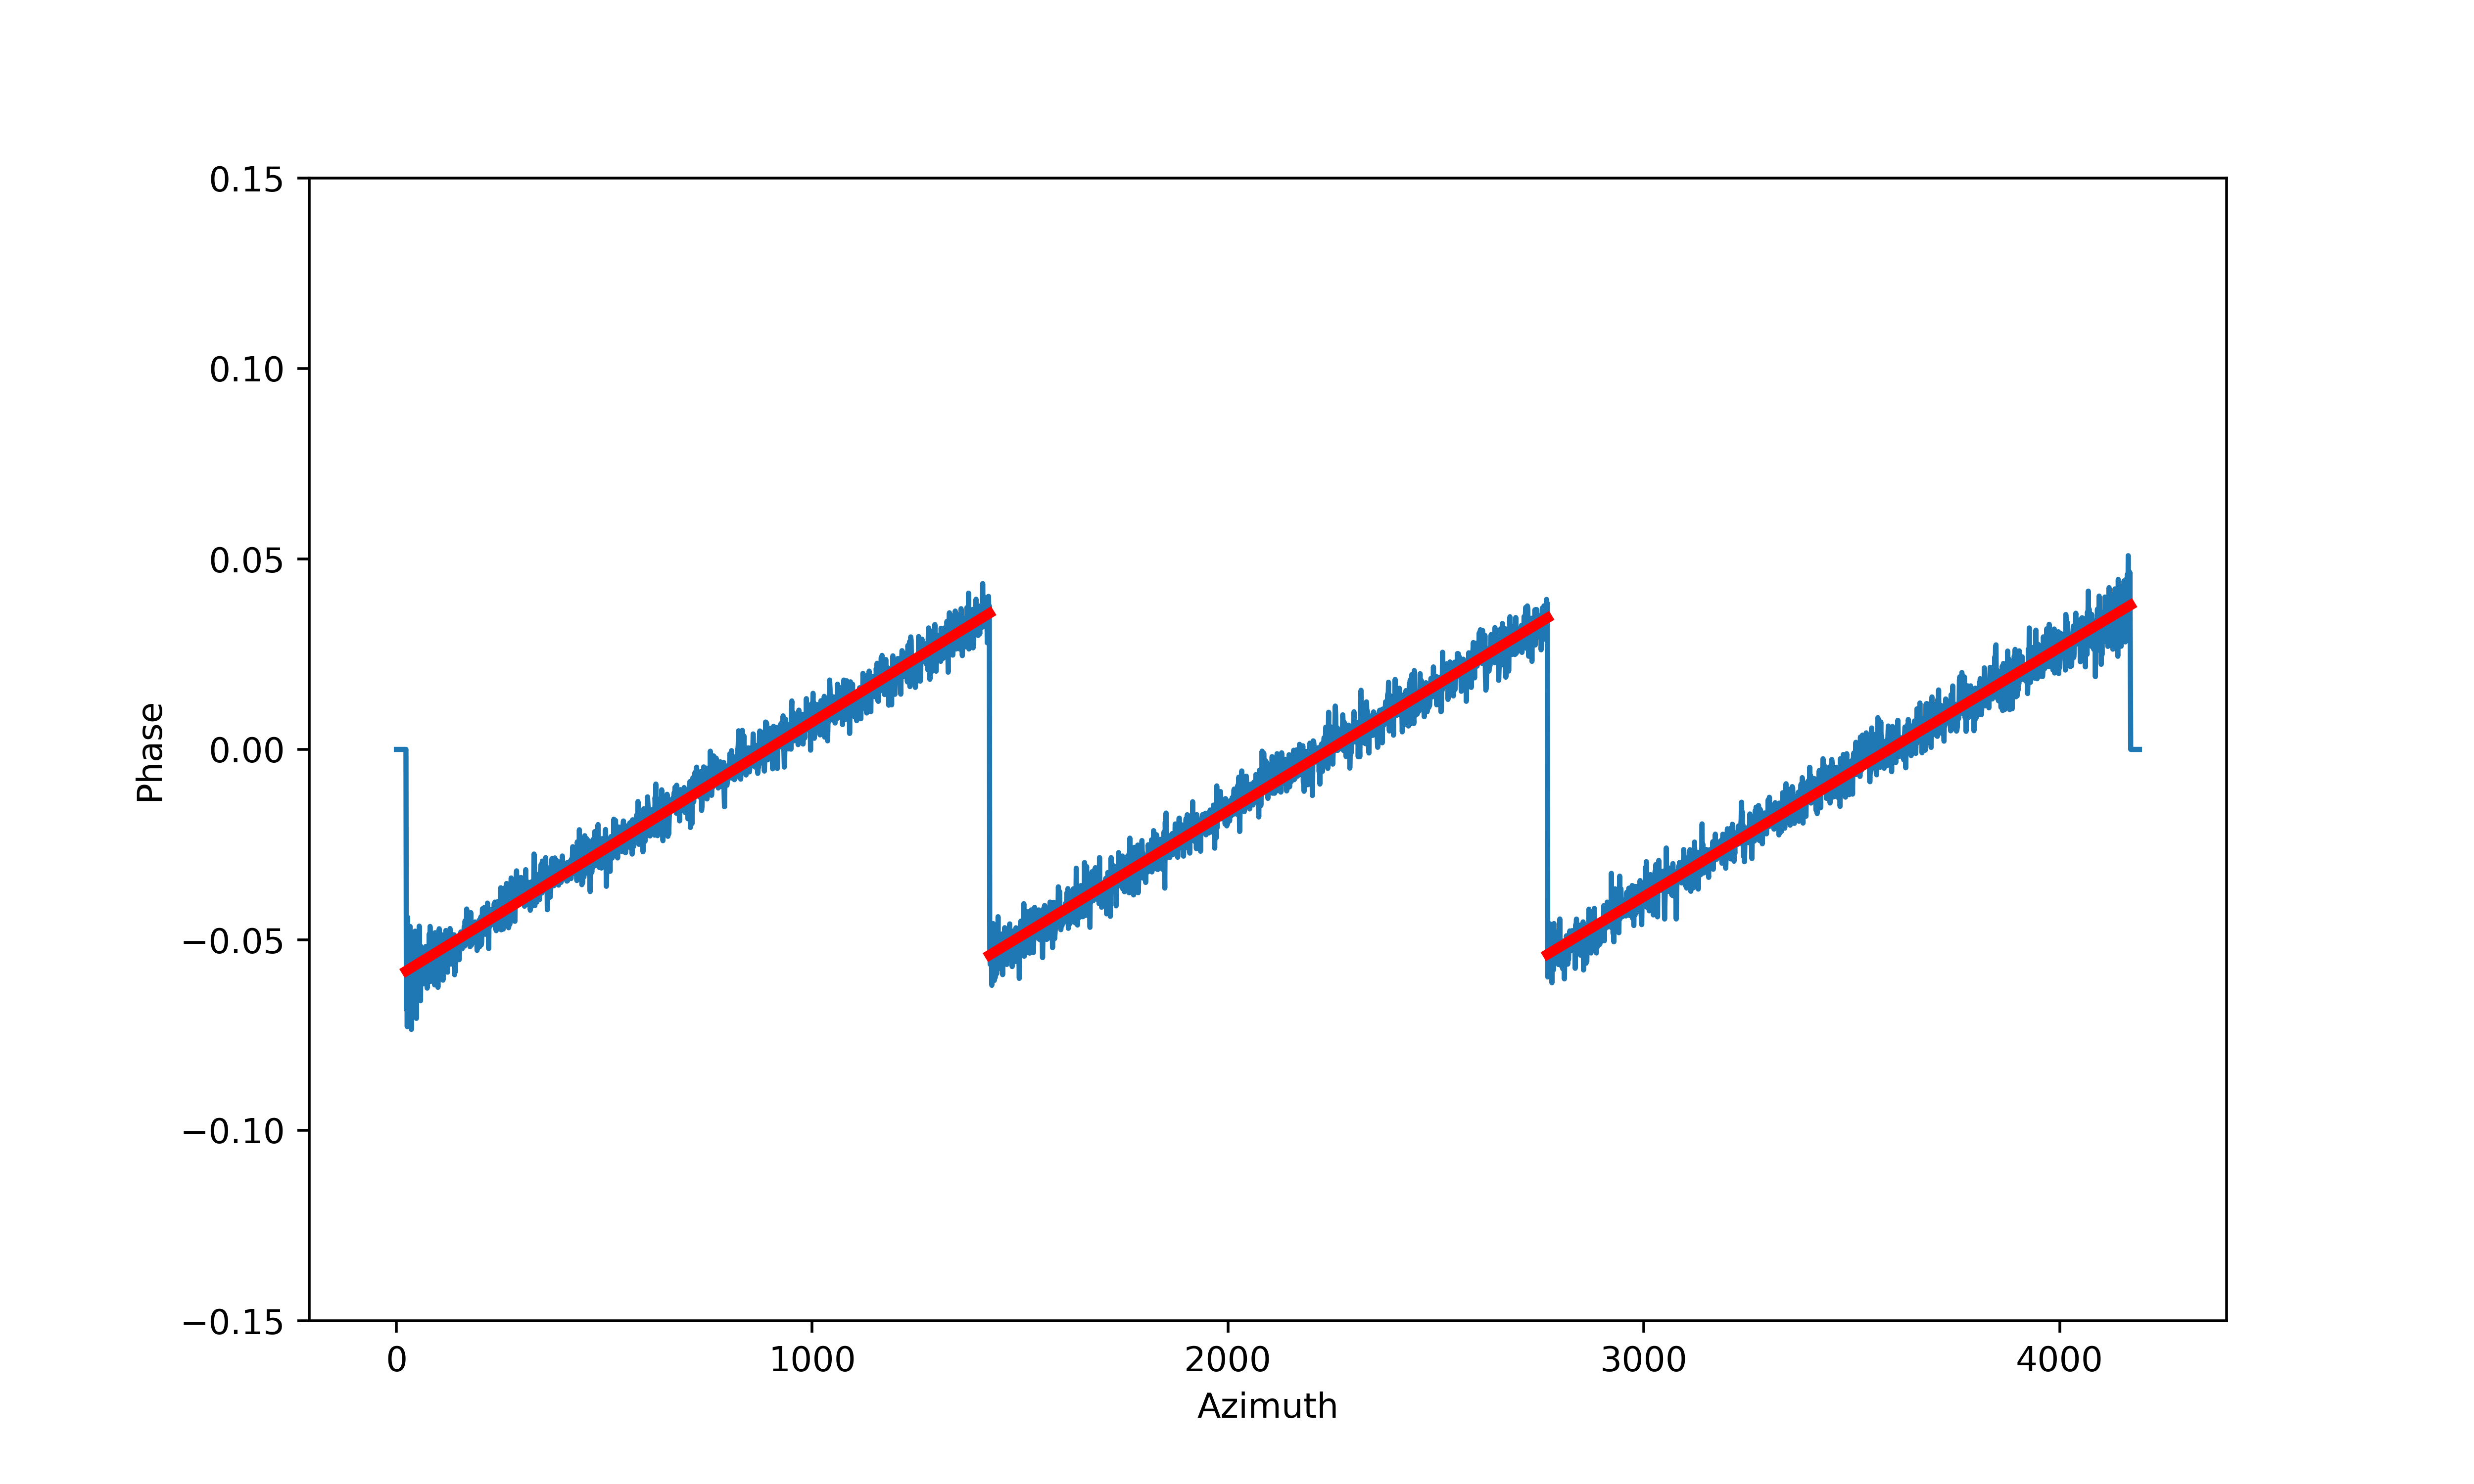
\includegraphics[width=\textwidth]{figure/The cross-interferogram/cross_interf_Milan_asc_row&fitted_20230104.png}
        \end{minipage}
        \caption{Milan ascending}
        \label{fig_5f}
    \end{subfigure}%
    \begin{subfigure}{0.5\textwidth}
        \centering
        \begin{minipage}{0.5\textwidth}
            \centering
            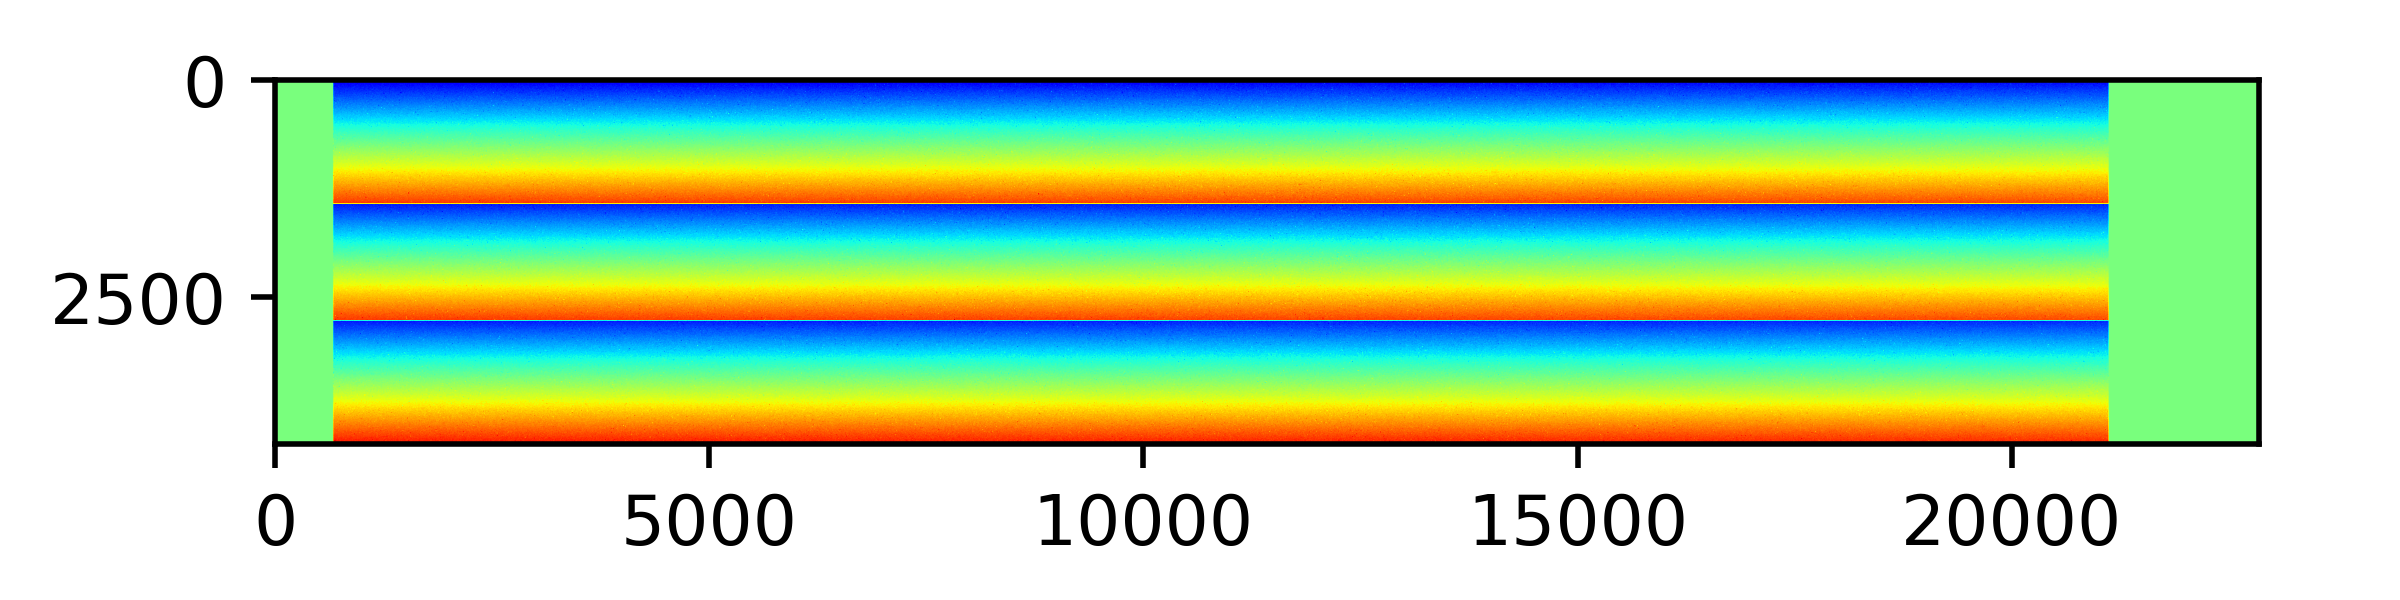
\includegraphics[width=\textwidth]{figure/The cross-interferogram/cross_interf_Milan_des.png}
        \end{minipage}%
        \begin{minipage}{0.5\textwidth}
            \centering
            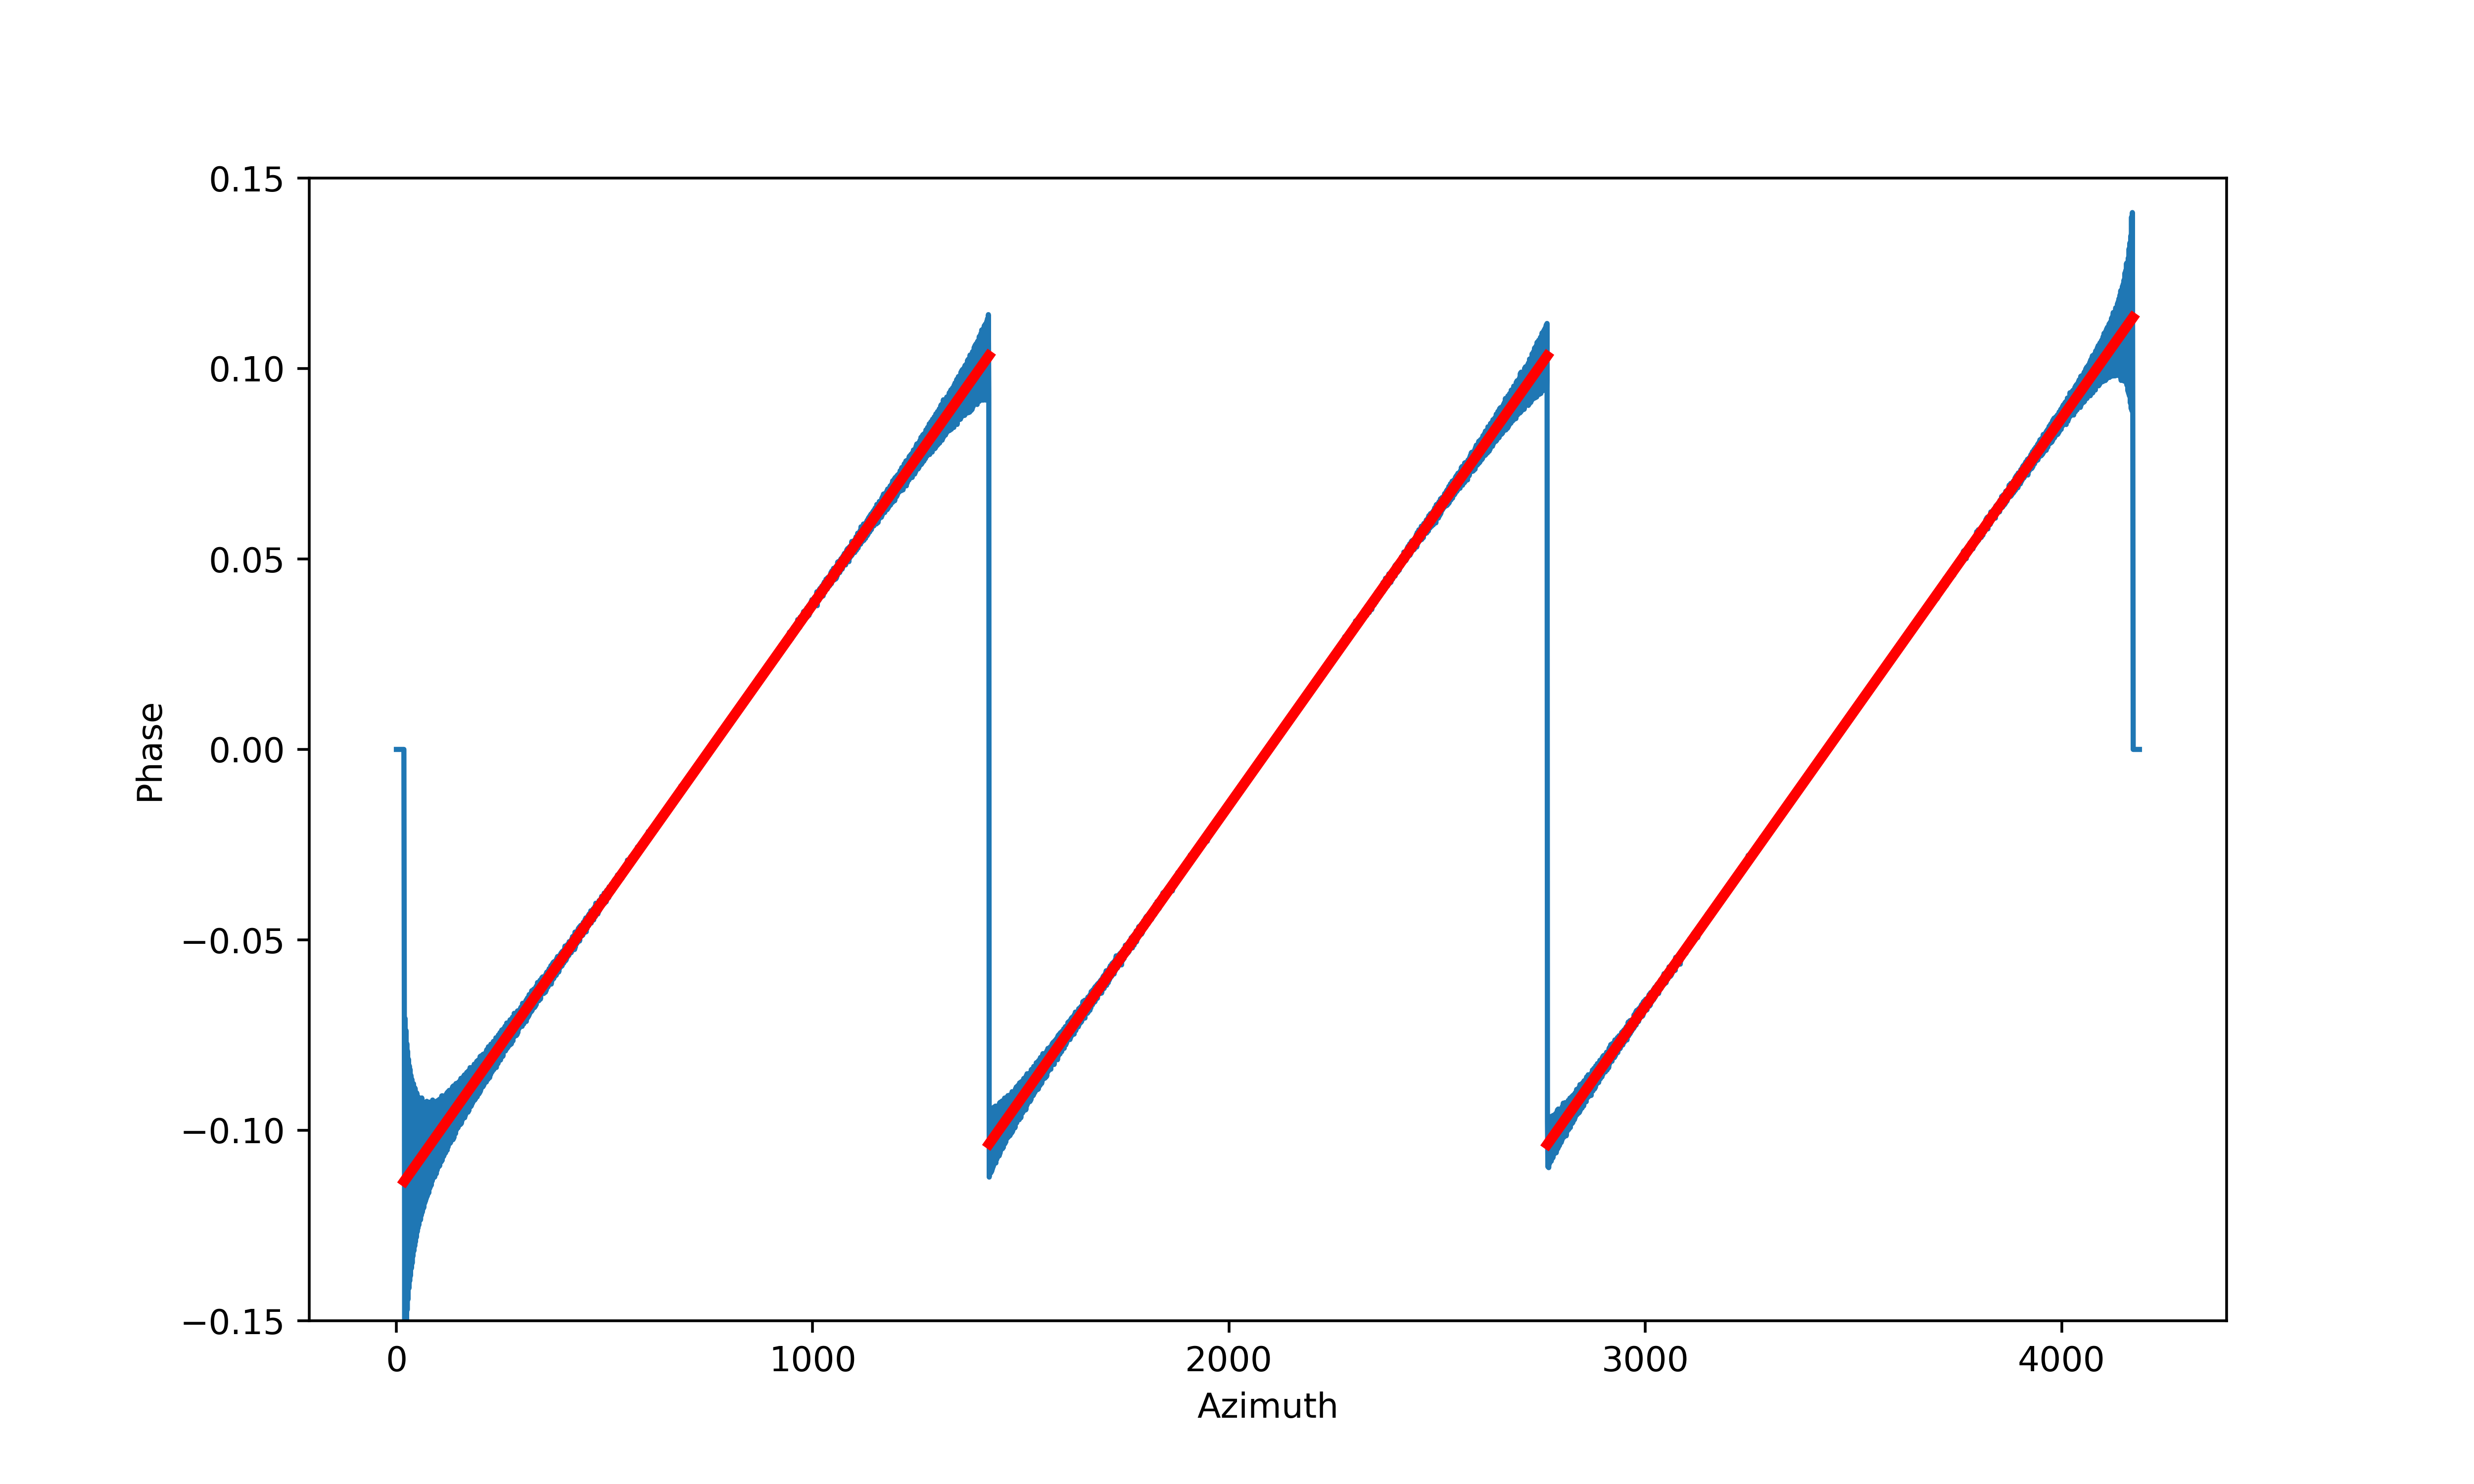
\includegraphics[width=\textwidth]{figure/The cross-interferogram/cross_interf_Milan_des_row&fitted_20230108.png}
        \end{minipage}
        \caption{Milan descending}
        \label{fig_5g}
    \end{subfigure}%
    \hfill
    \begin{subfigure}{0.5\textwidth}
        \centering
        \begin{minipage}{0.5\textwidth}
            \centering
            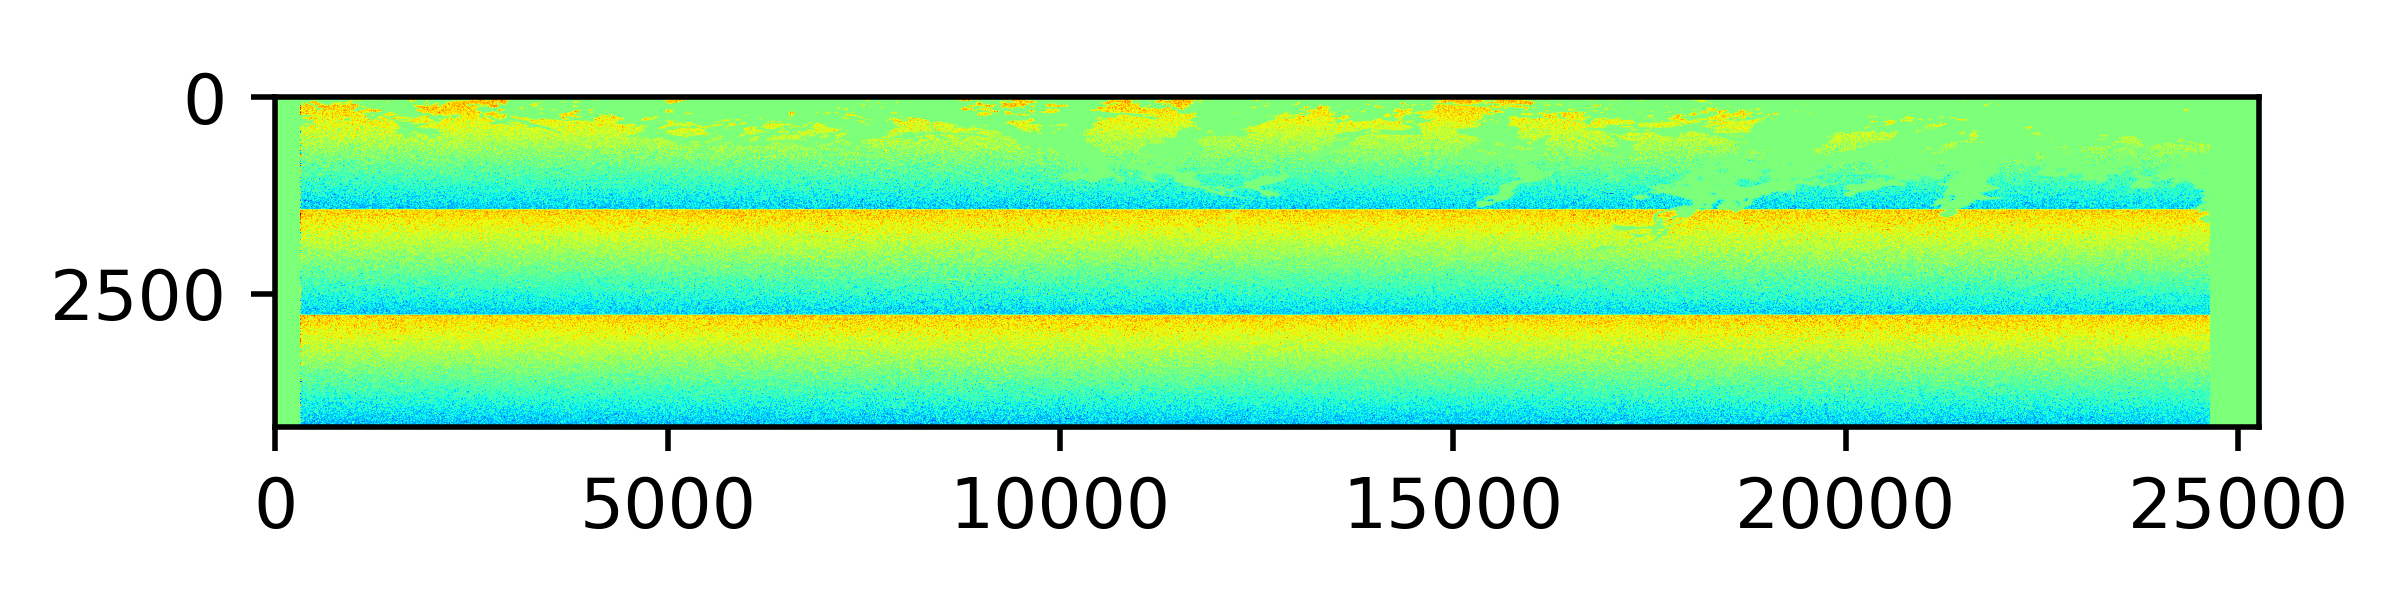
\includegraphics[width=\textwidth]{figure/The cross-interferogram/cross_interf_Finland_asc.png}
        \end{minipage}%
        \begin{minipage}{0.5\textwidth}
            \centering
            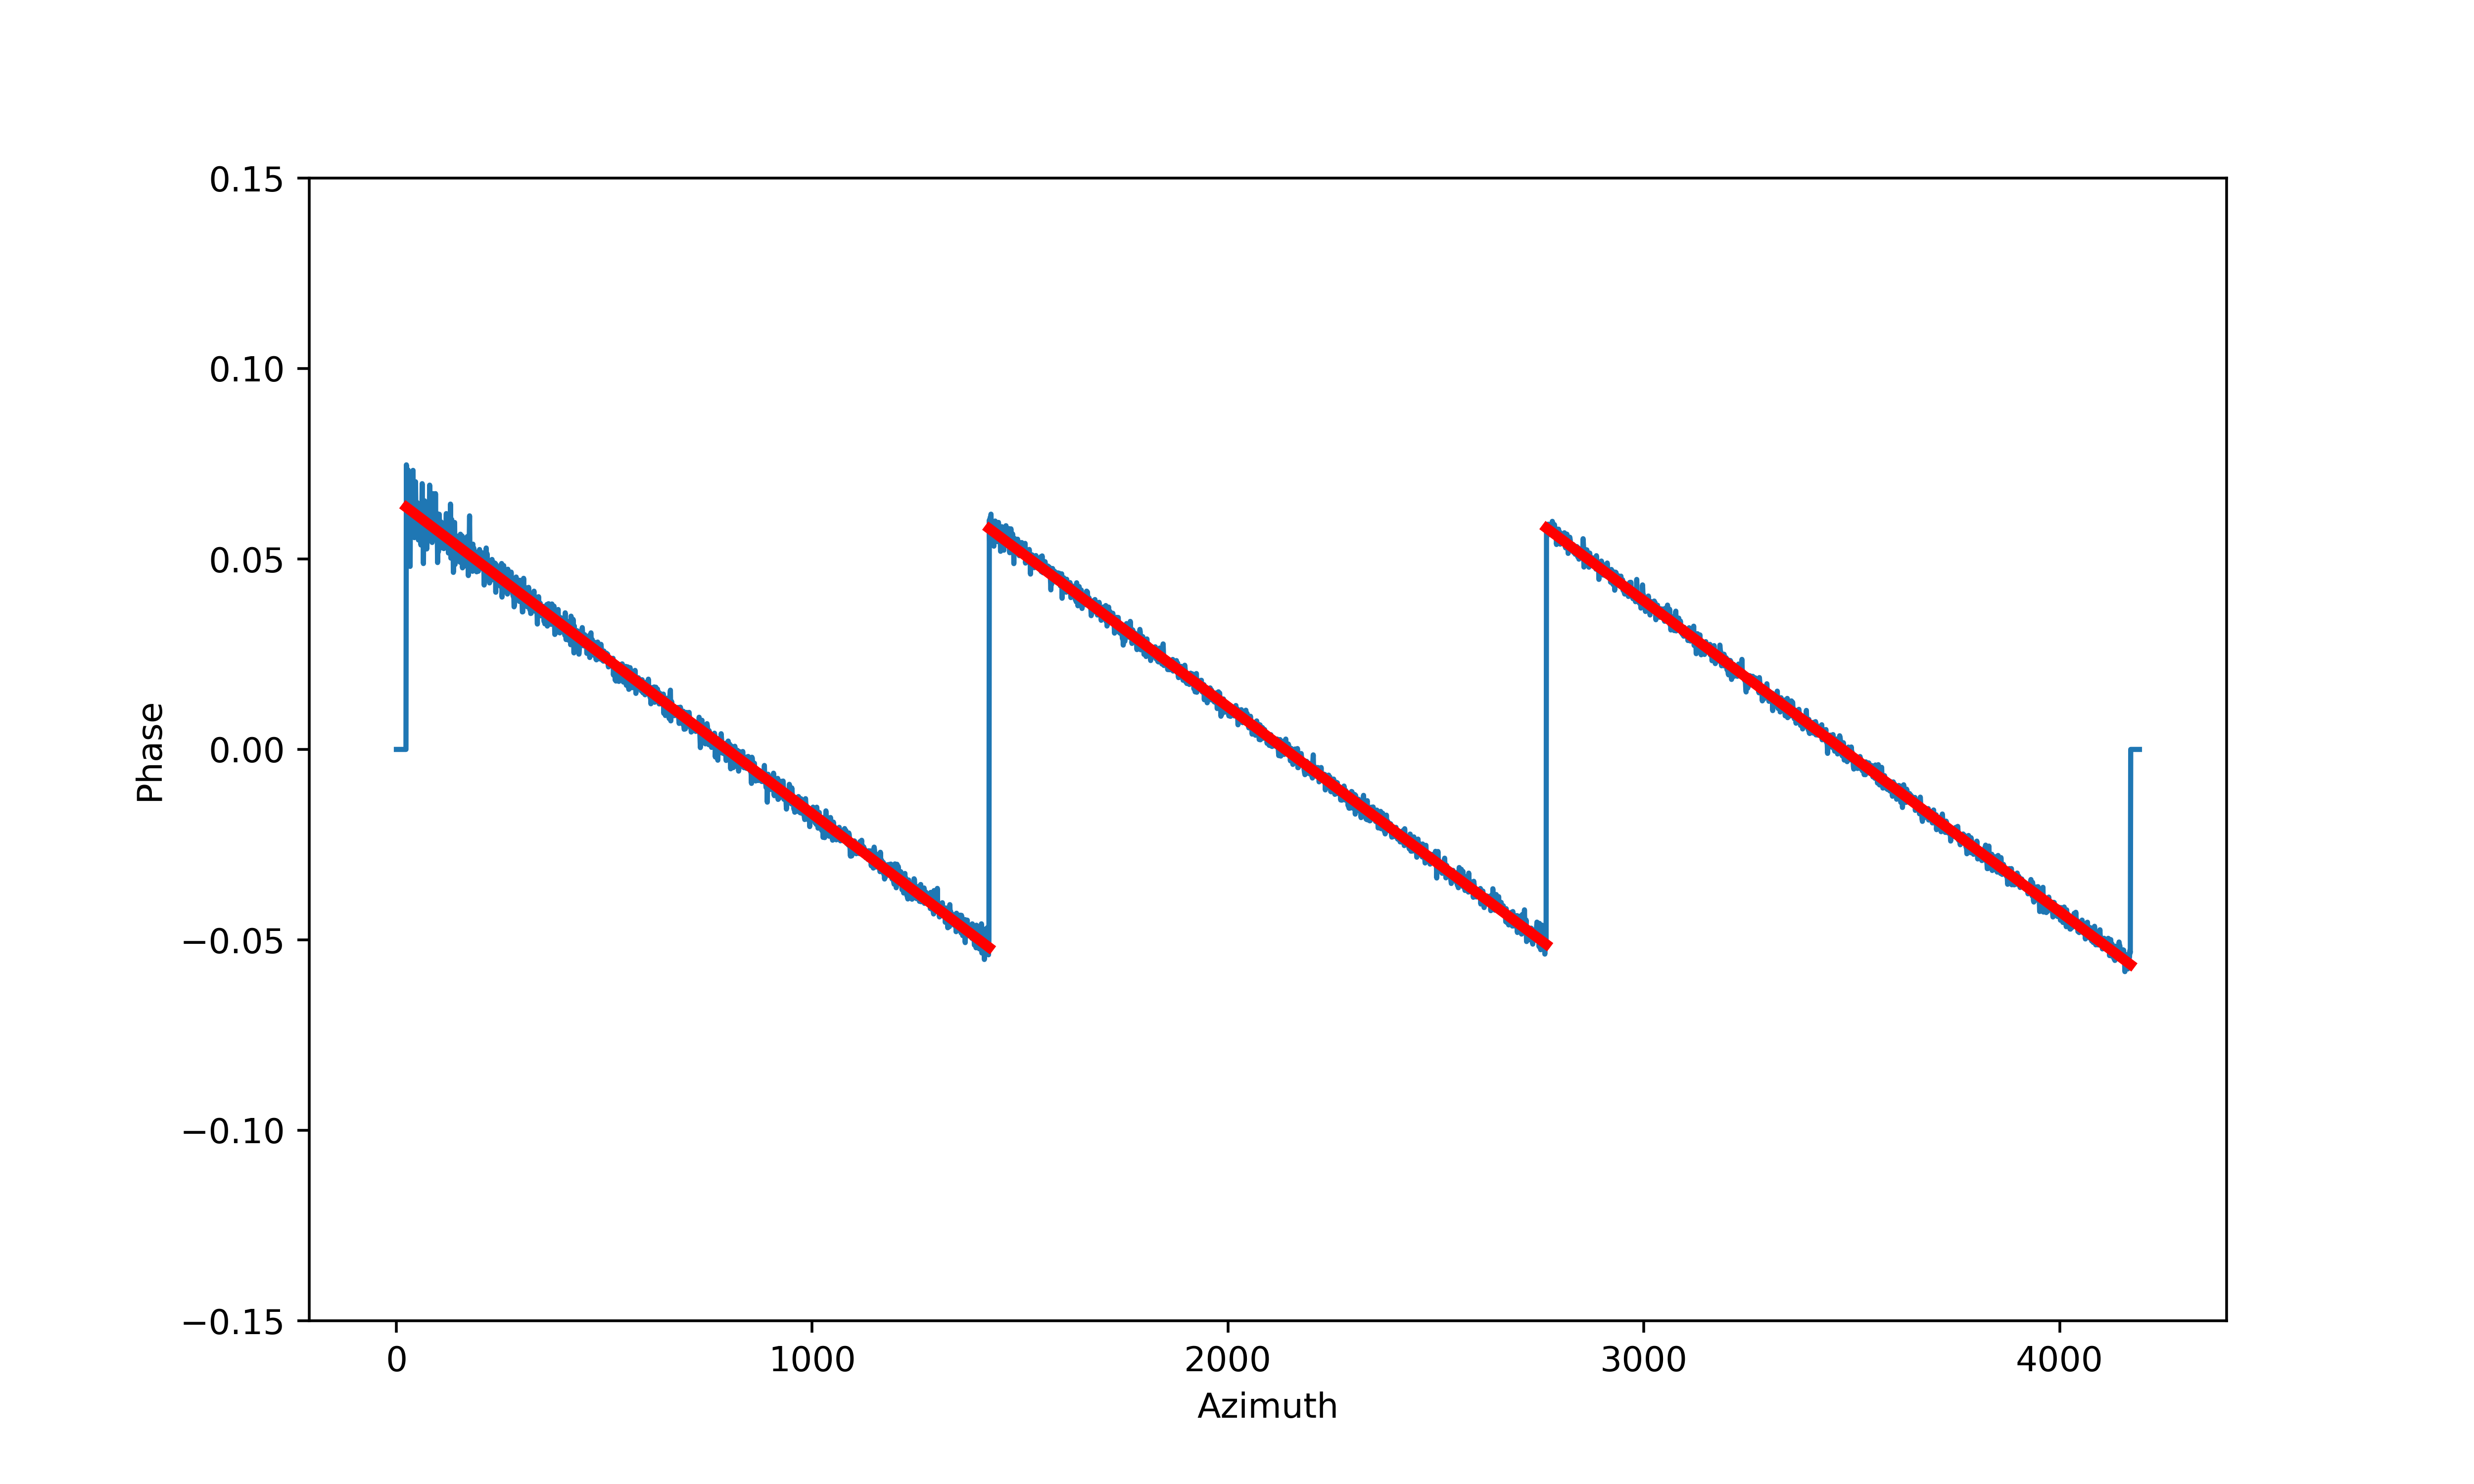
\includegraphics[width=\textwidth]{figure/The cross-interferogram/cross_interf_Finland_asc_row&fitted_20230102.png}
        \end{minipage}
        \caption{Finland ascending}
        \label{fig_5h}
    \end{subfigure}%
    \begin{subfigure}{0.5\textwidth}
        \centering
        \begin{minipage}{0.5\textwidth}
            \centering
            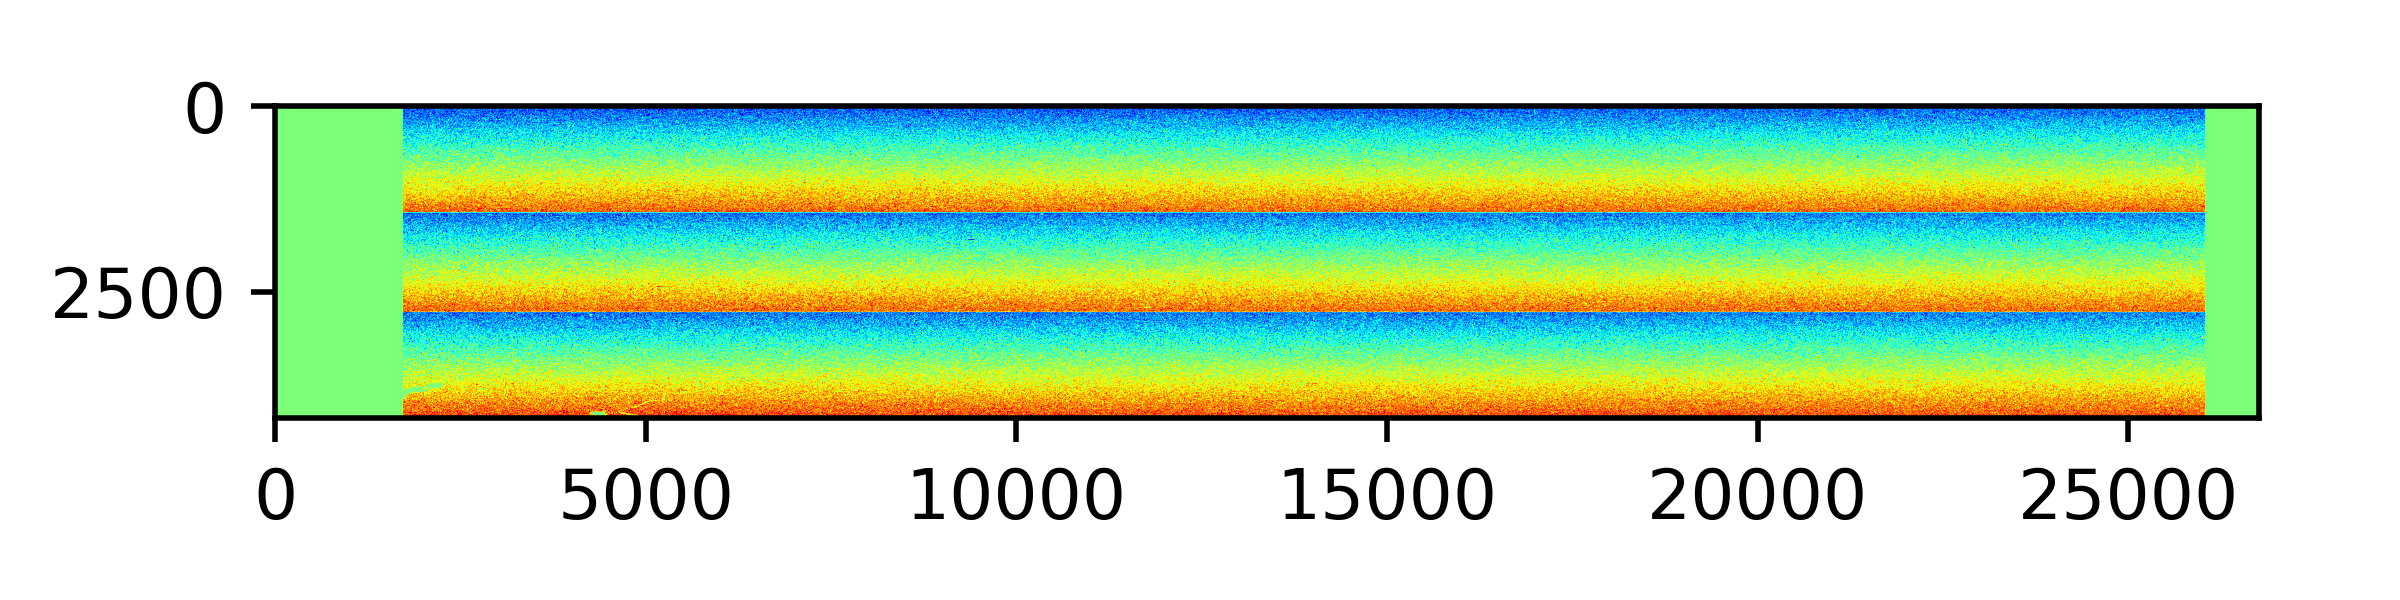
\includegraphics[width=\textwidth]{figure/The cross-interferogram/cross_interf_Finland_des.png}
        \end{minipage}%
        \begin{minipage}{0.5\textwidth}
            \centering
            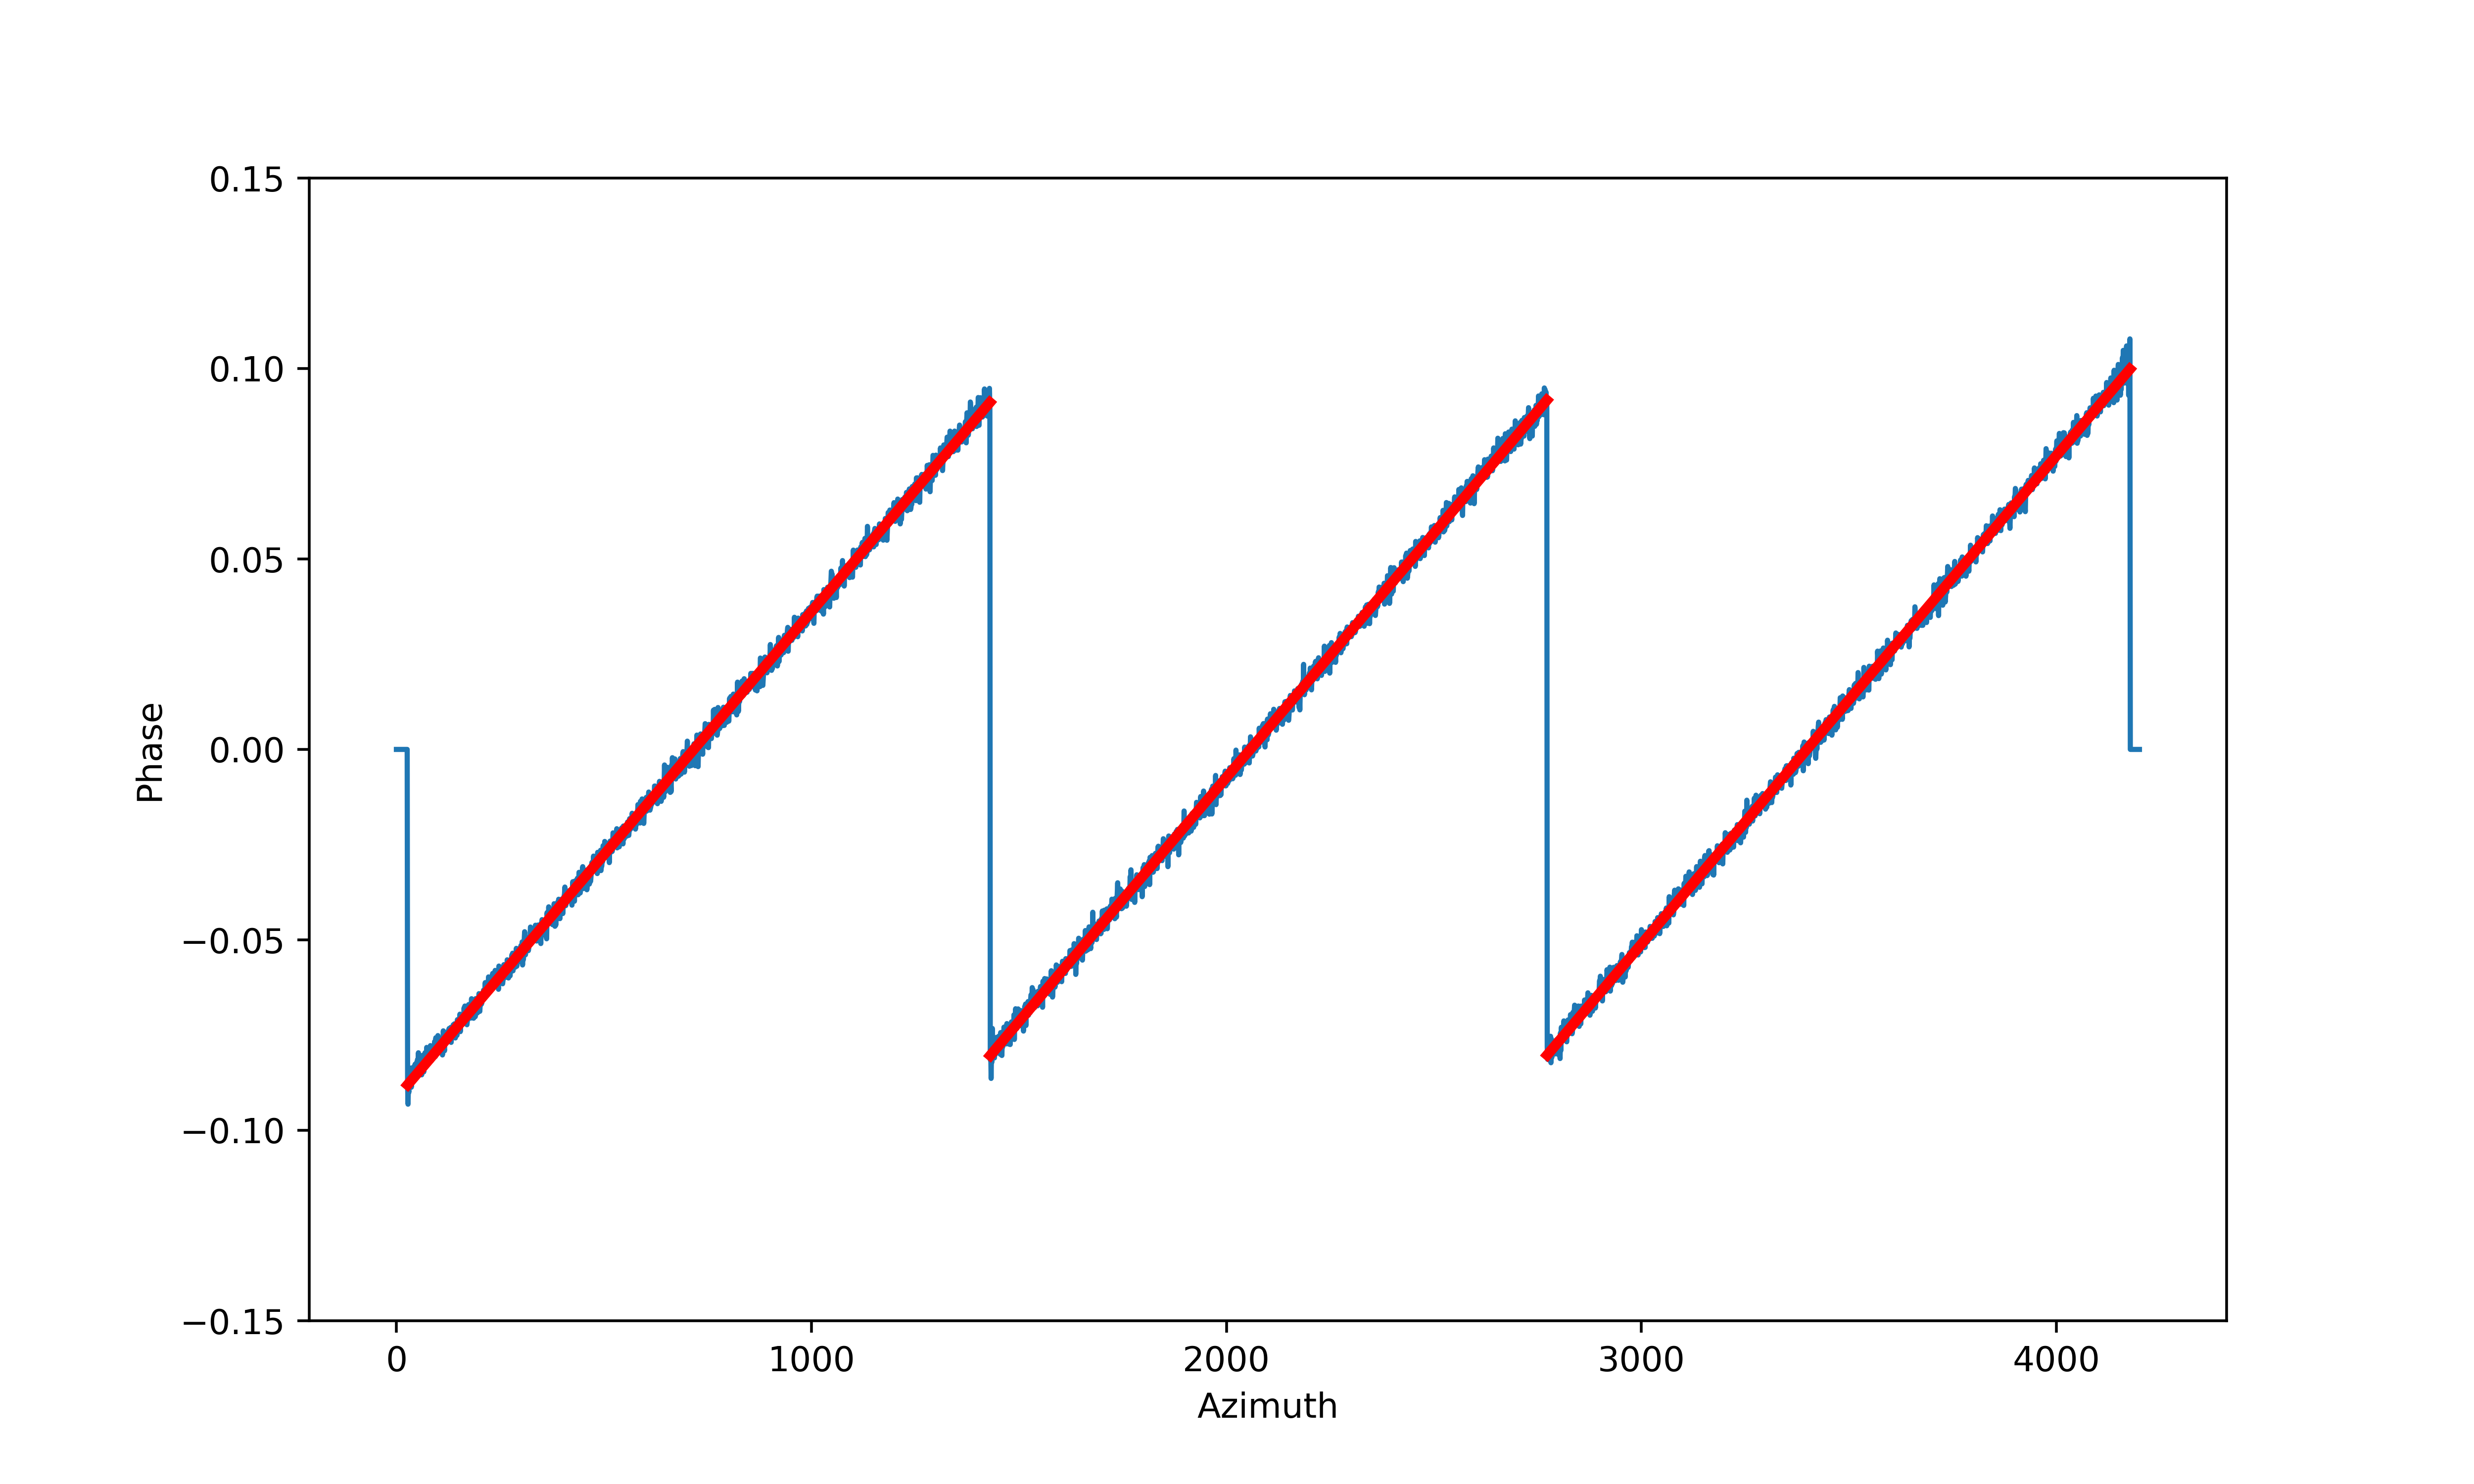
\includegraphics[width=\textwidth]{figure/The cross-interferogram/cross_interf_Finland_des_row&fitted_20230102.png}
        \end{minipage}
        \caption{Finland descending}
        \label{fig_5i}
    \end{subfigure}%
    \caption{The cross-interferogram (Note: Taklamakan desert descending data is incomplete, and the results are selected from July 2022 to January 2023)}
    \label{fig_5}
\end{figure}

It is challenging to assess whether the phase is accurate by visual criteria alone \cite{An_enhanced_spectral_diversity_coregistration_method_for_dual-polarimetric_Sentinel-1A/B_TOPS_data}. At the same time, ESD realizes the weight determination through coherence during the migration process. Therefore, coherence distribution is also a sign to measure the experimental results. The coherence and its distribution of each study area from January 2022 to January 2023 are selected as reference, as shown in \ref{fig_6}. From the coherence, it can be clearly judged that the urban area has high coherence, and the higher the vegetation coverage, the lower the coherence. It is speculated that the azimuth shift is greatly affected by the urban area, and the reliability of the shift is strong when the urban area is stable. Regardless of the type of study area, the coherence of the entire image covered is concentrated between 0 and 0.6. It can be inferred from \ref{eq_6} that low coherence may lead to higher ESD miscoregistration and worse stability of coregistration results. Therefore, this point needs to be considered in coregistration. \par

\begin{figure}
    \centering
    \begin{subfigure}[c]{0.5\textwidth}
        \centering
        \begin{minipage}[c]{0.5\textwidth}
            \centering
            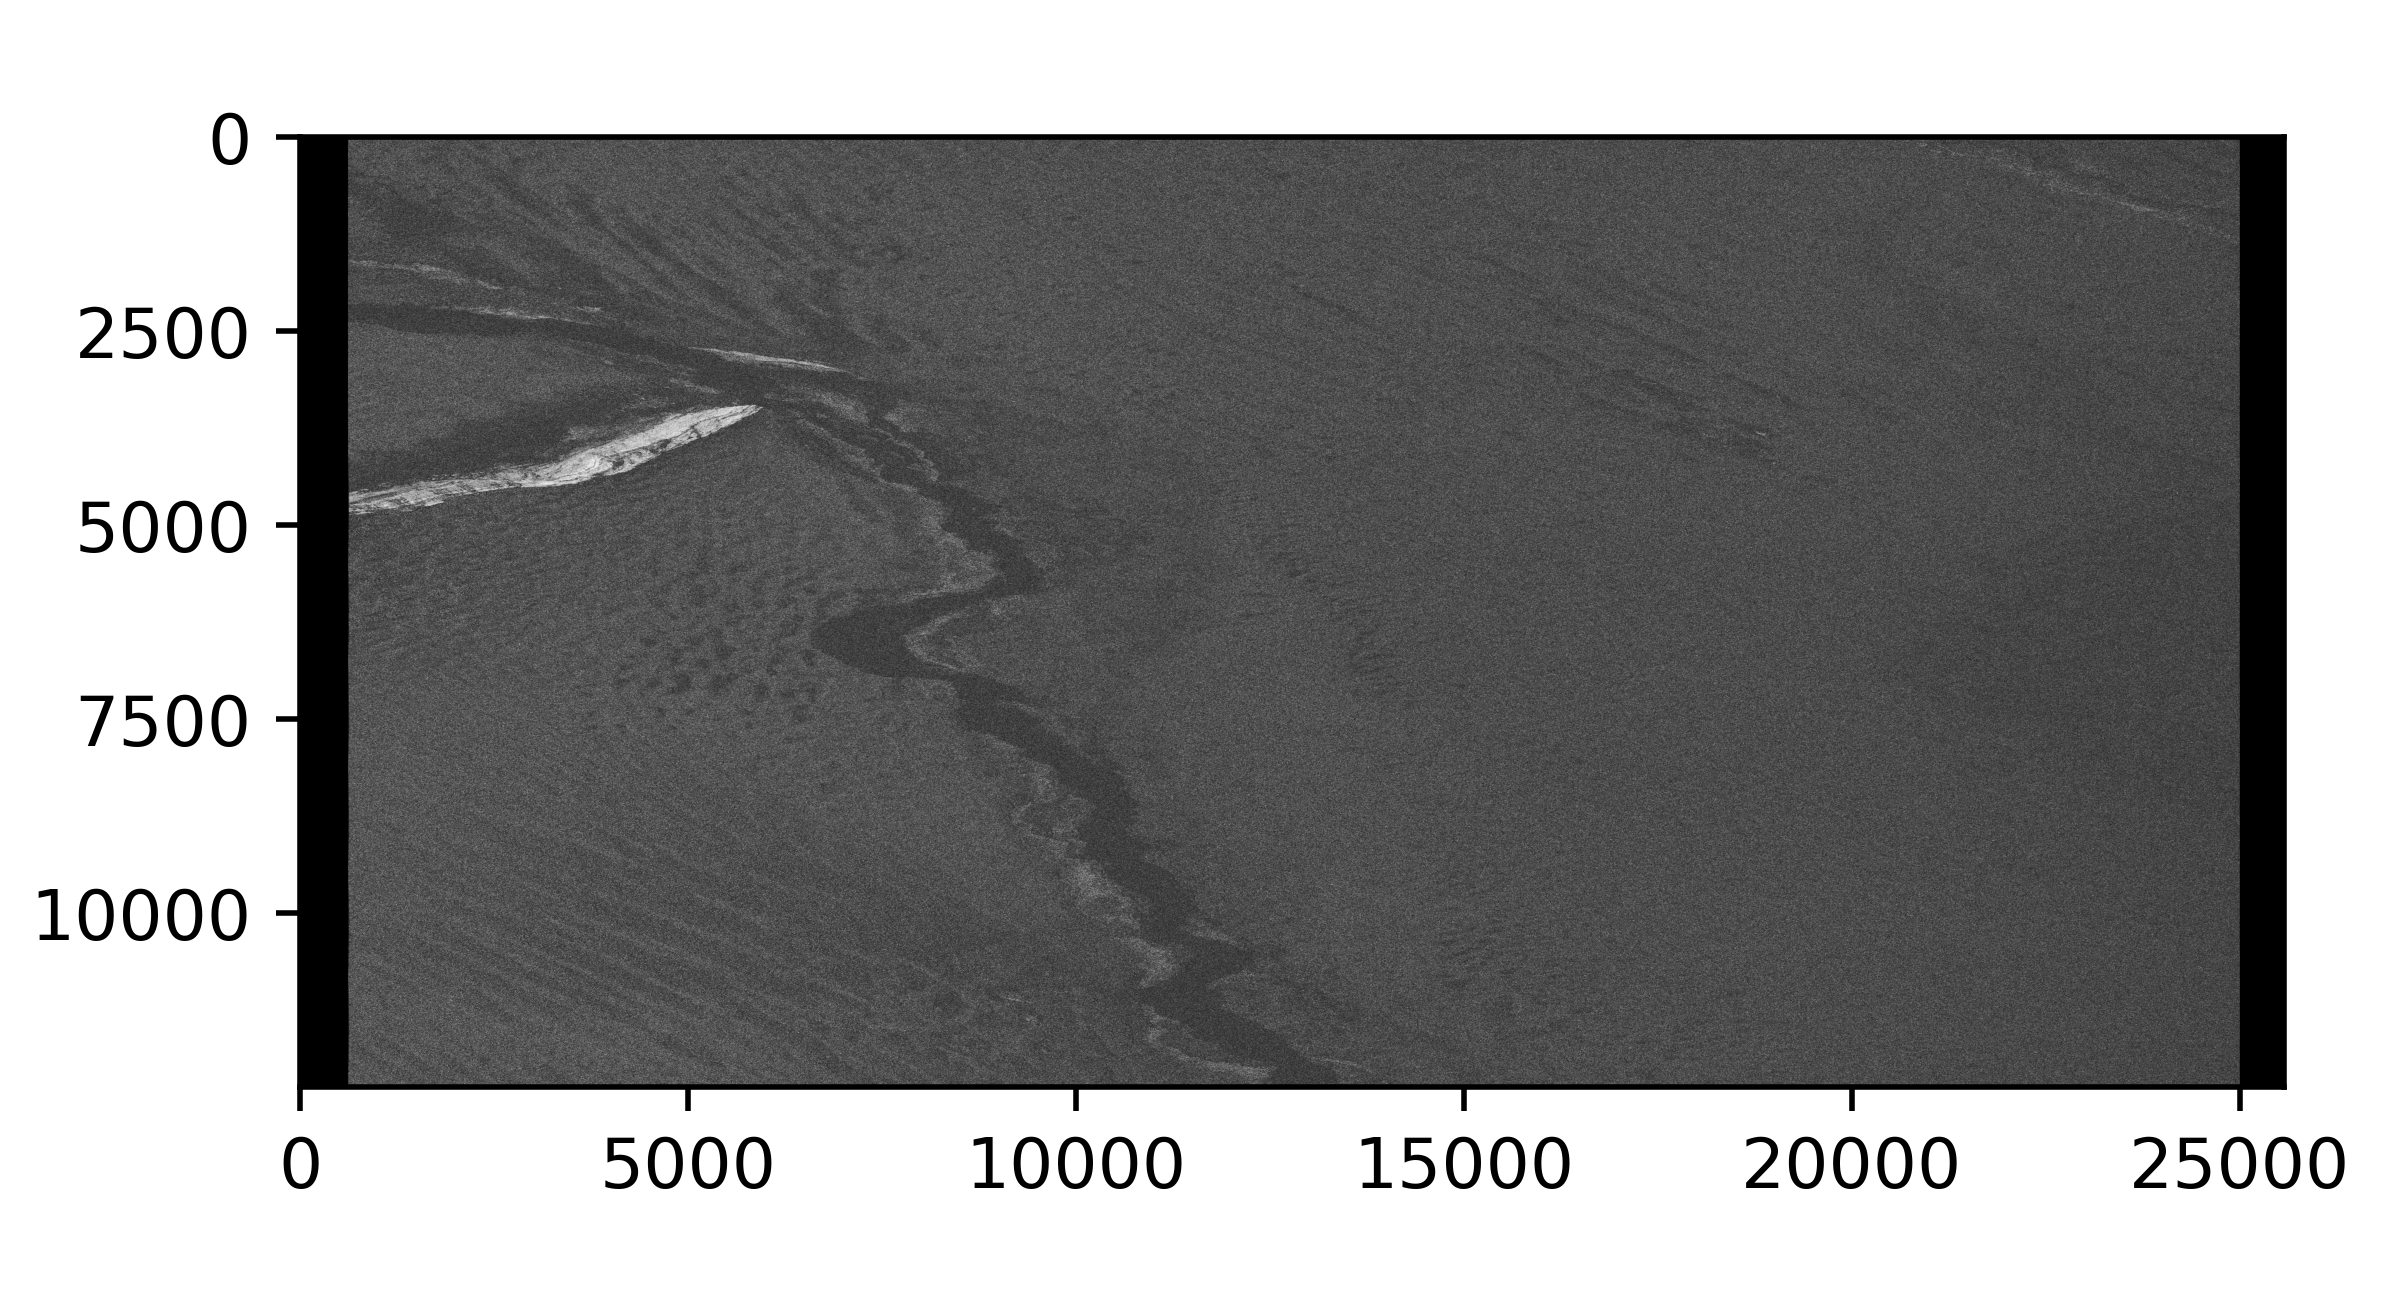
\includegraphics[width=\textwidth]{figure/The coherence/coh_TaklimakanDesert_asc_esd1.png}
        \end{minipage}%
        \begin{minipage}[c]{0.5\textwidth}
            \centering
            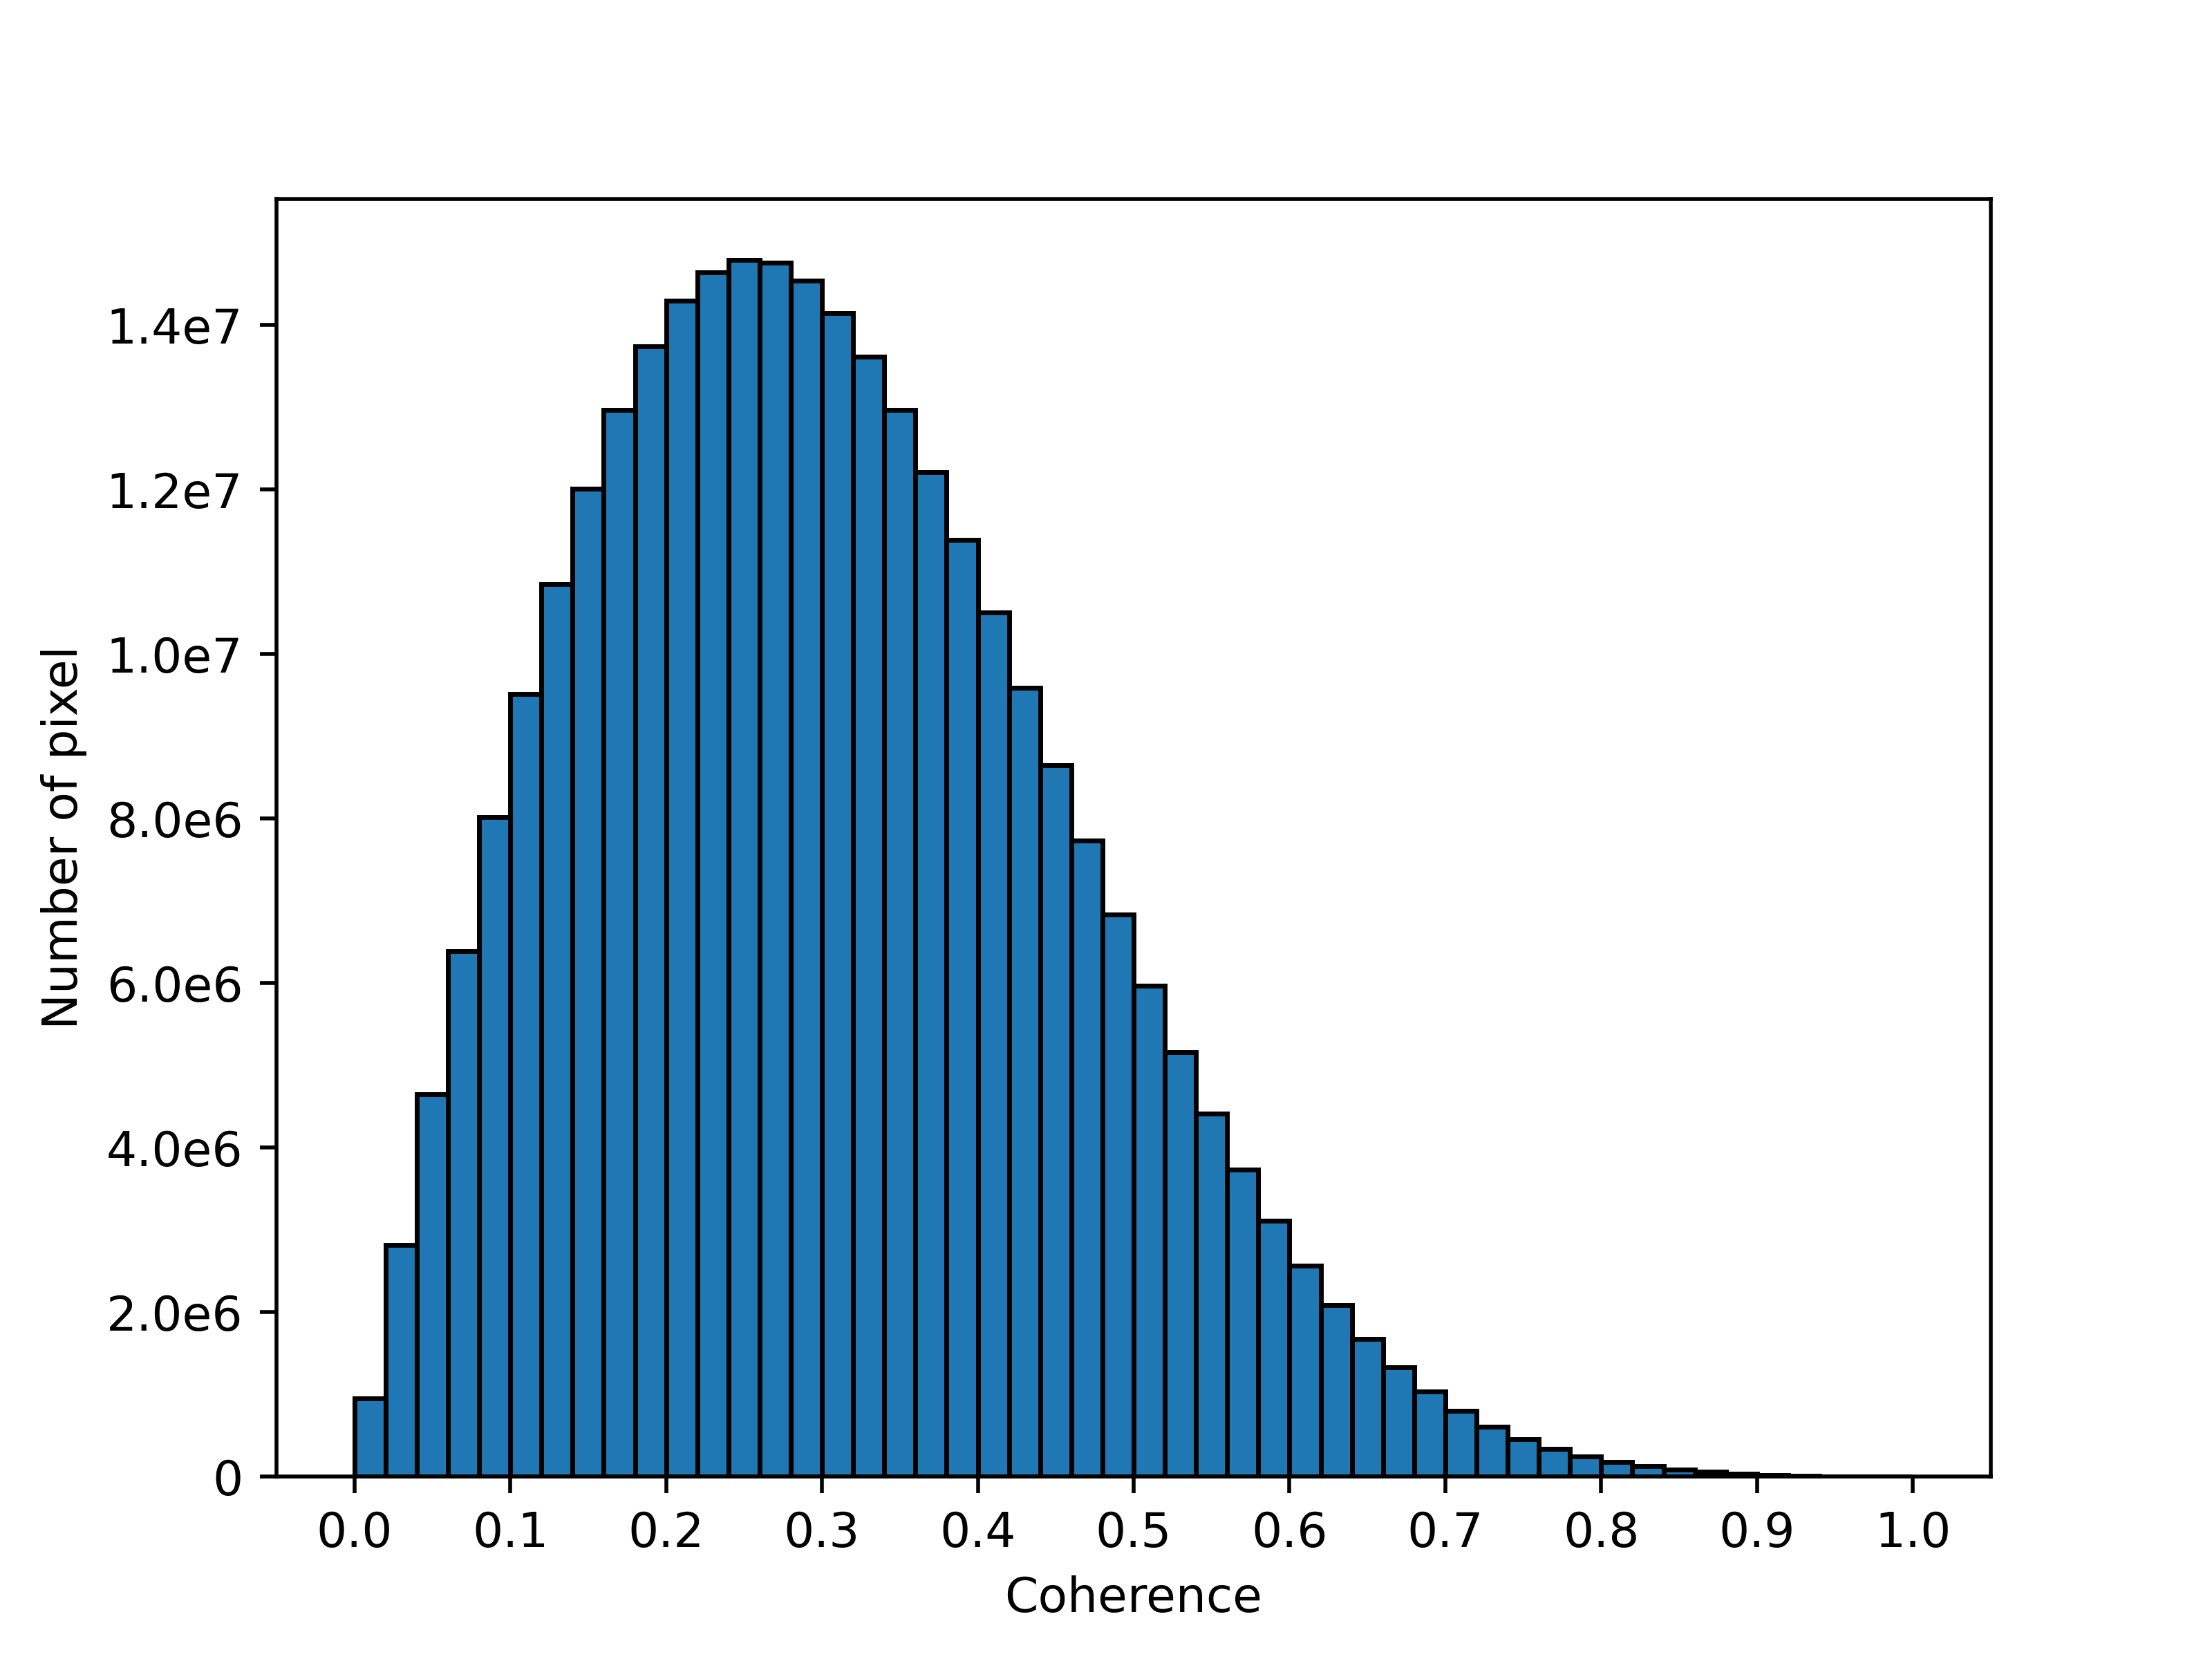
\includegraphics[width=\textwidth]{figure/The coherence/coh_TaklimakanDesert_asc_esd1_histogram_.png}
        \end{minipage}
        \caption{Taklamakan desert ascending}
        \label{fig_6a}
    \end{subfigure}%
    \begin{subfigure}[c]{0.5\textwidth}
        \centering
        \begin{minipage}[c]{0.5\textwidth}
            \centering
            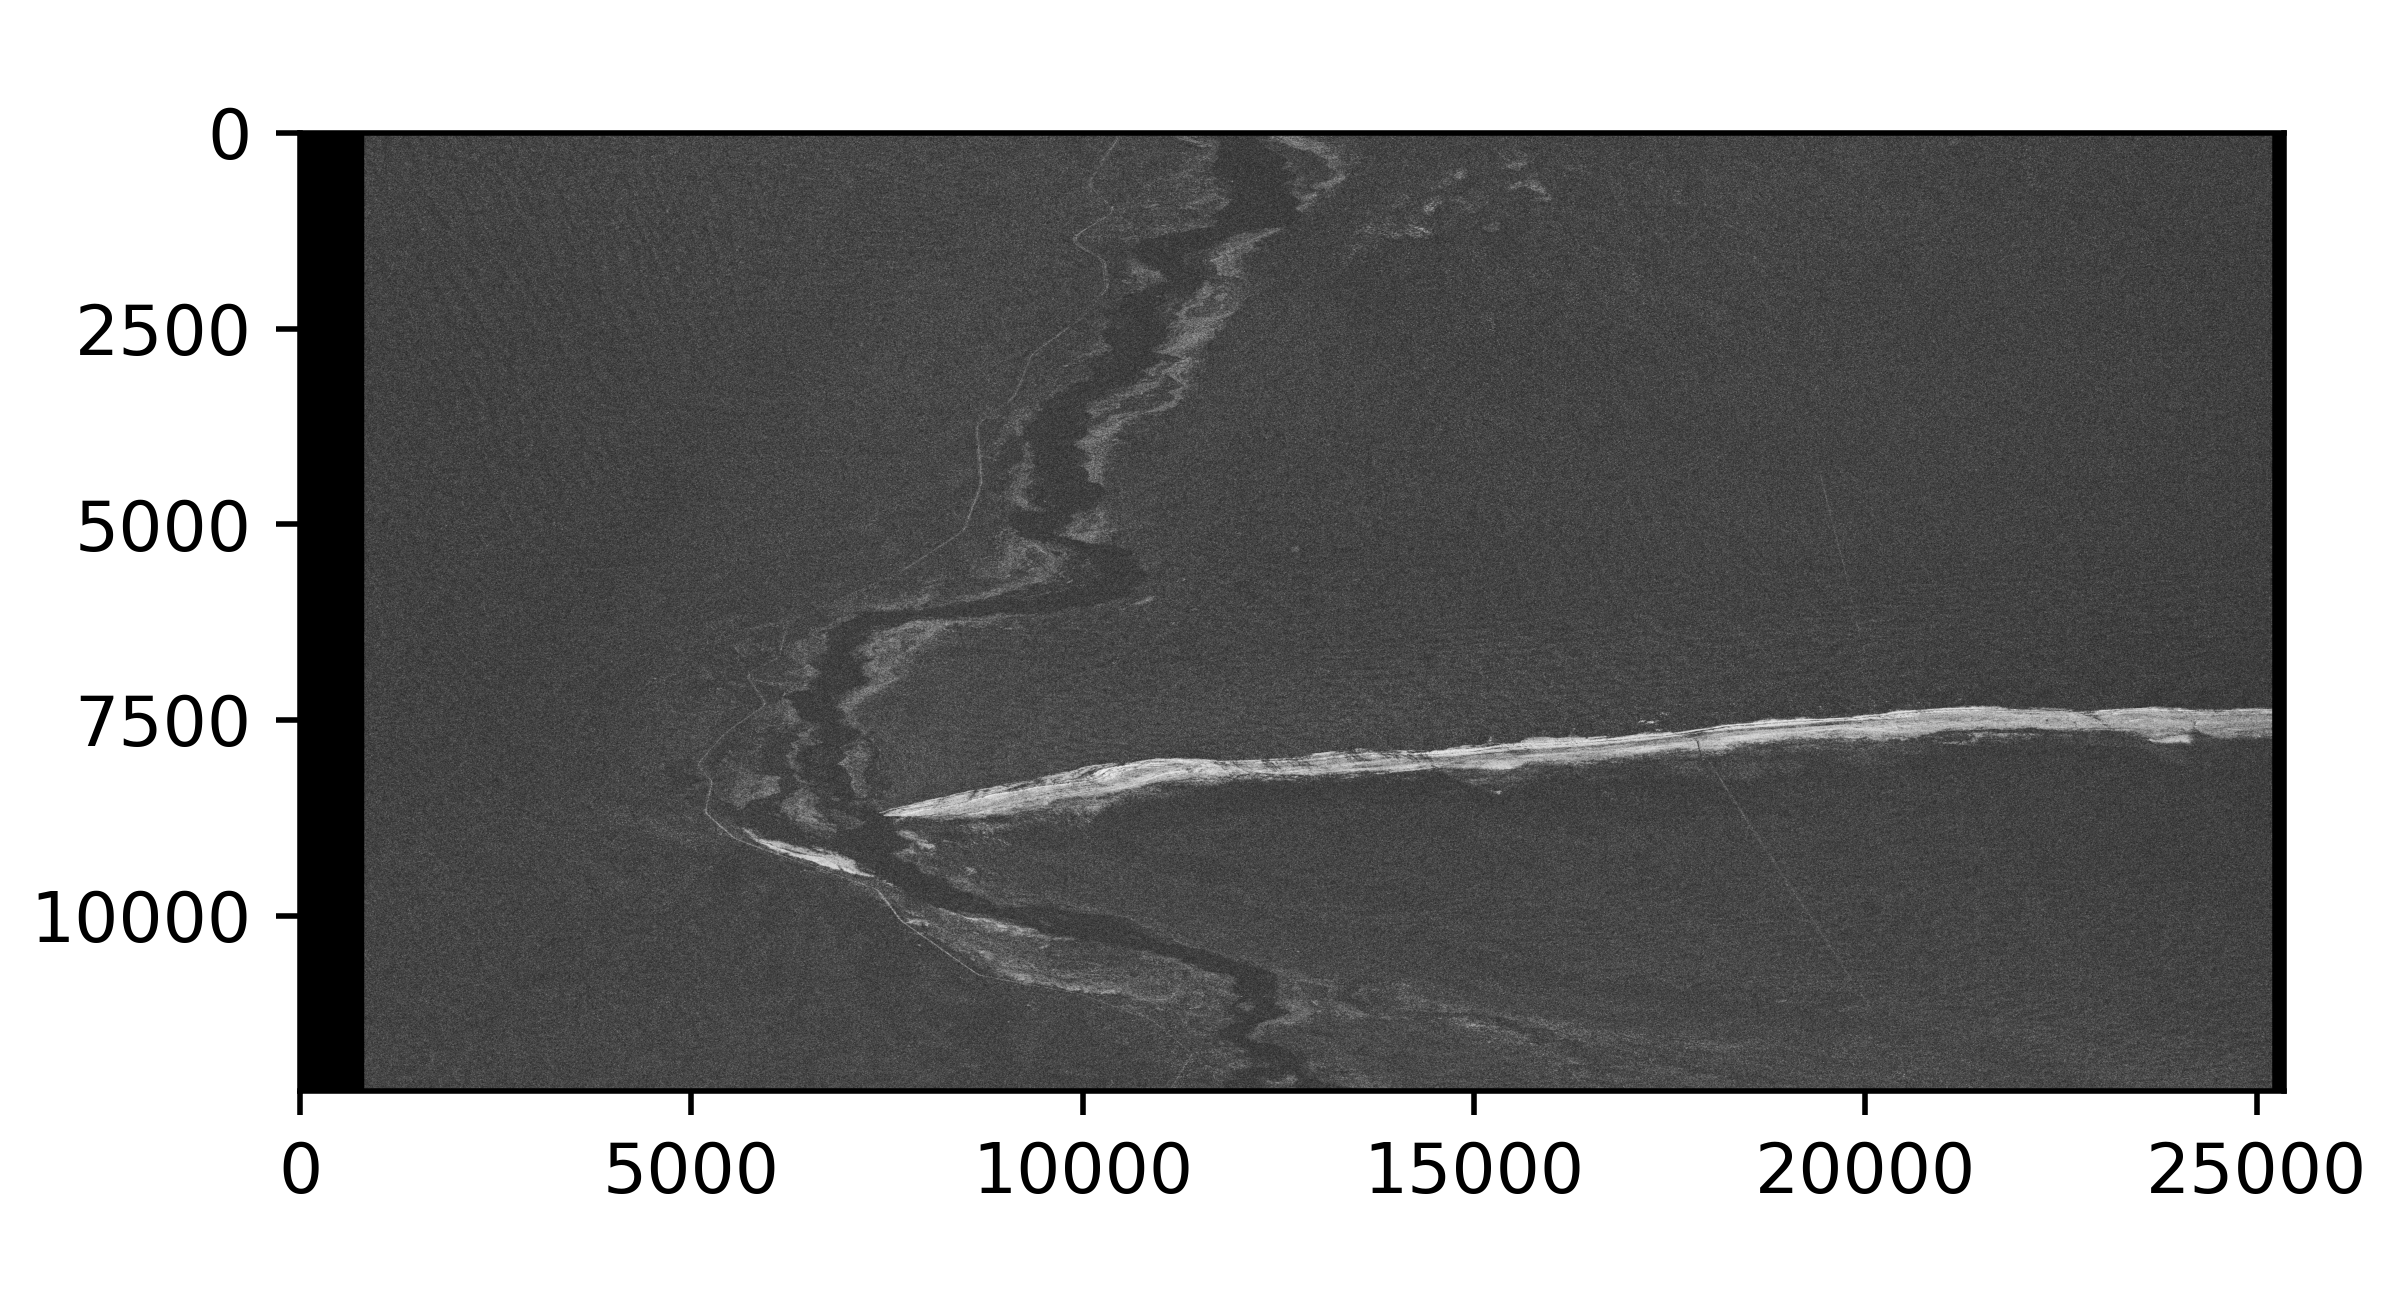
\includegraphics[width=\textwidth]{figure/The coherence/coh_TaklimakanDesert_des_esd1.png}
        \end{minipage}%
        \begin{minipage}[c]{0.5\textwidth}
            \centering
            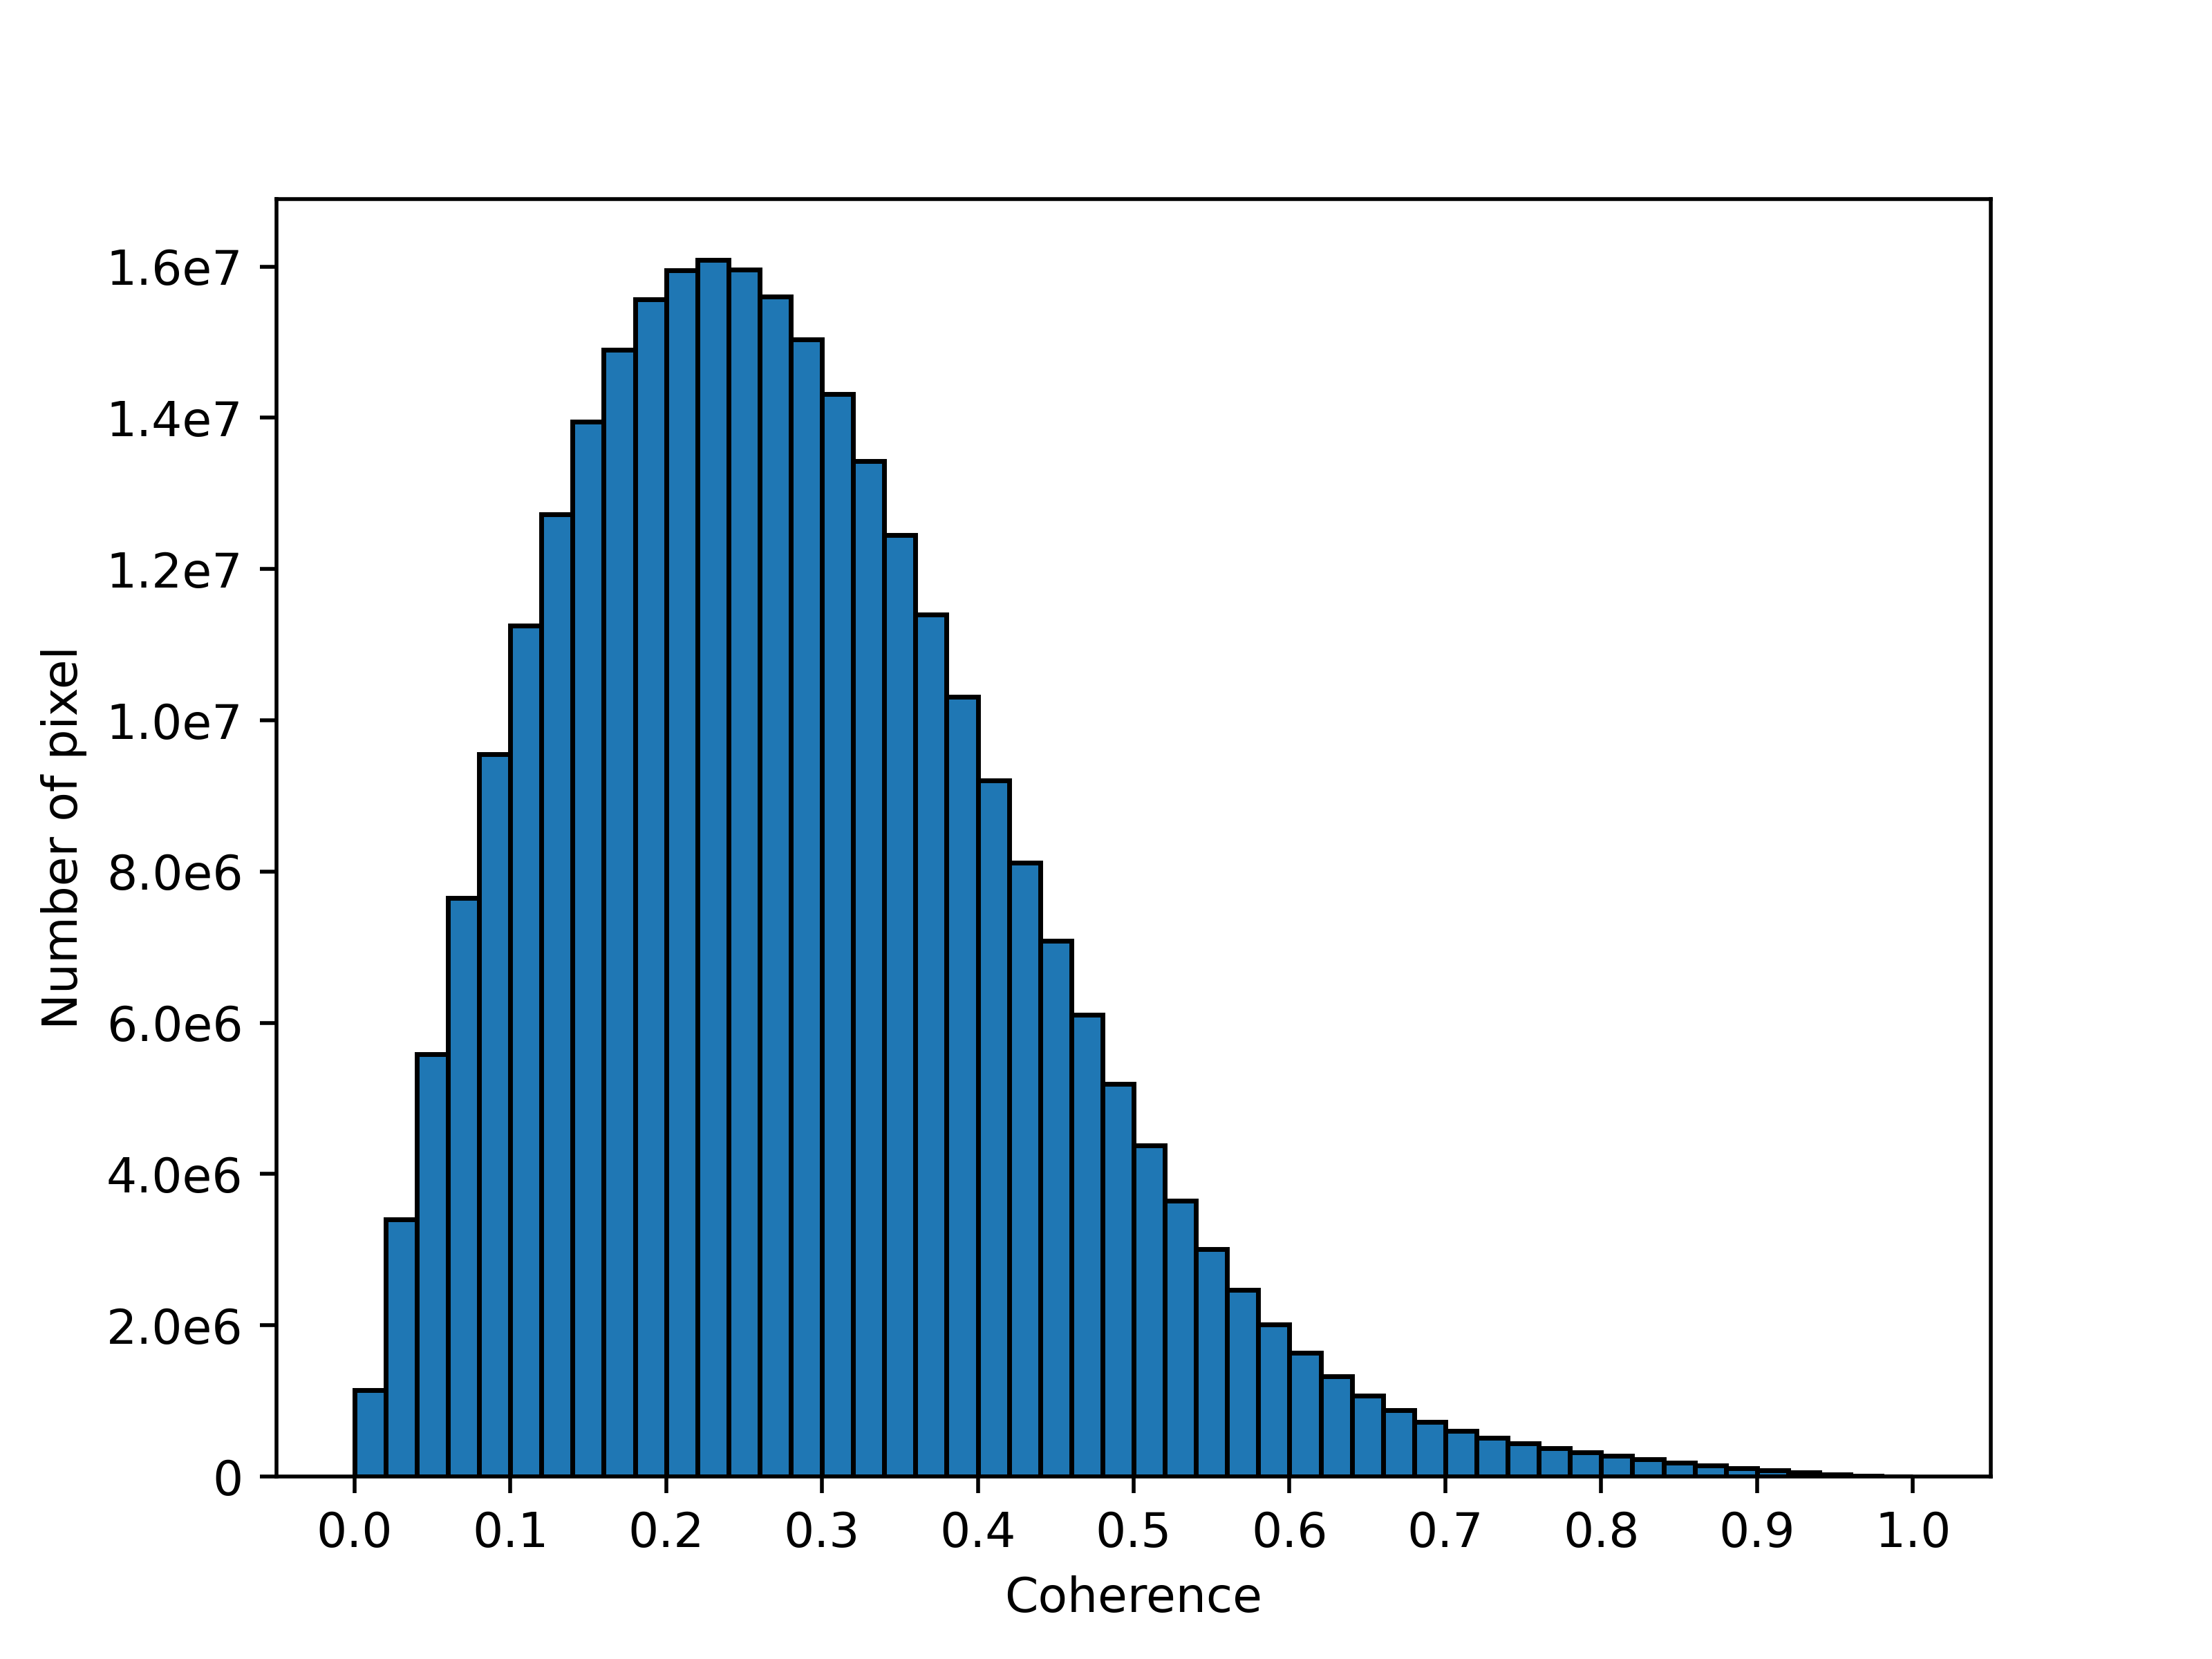
\includegraphics[width=\textwidth]{figure/The coherence/coh_TaklimakanDesert_des_esd1_histogram_.png}
        \end{minipage}
        \caption{Taklamakan desert descending}
        \label{fig_6b}
    \end{subfigure}%
    \hfill
    \begin{subfigure}{0.5\textwidth}
        \centering
        \begin{minipage}{0.5\textwidth}
            \centering
            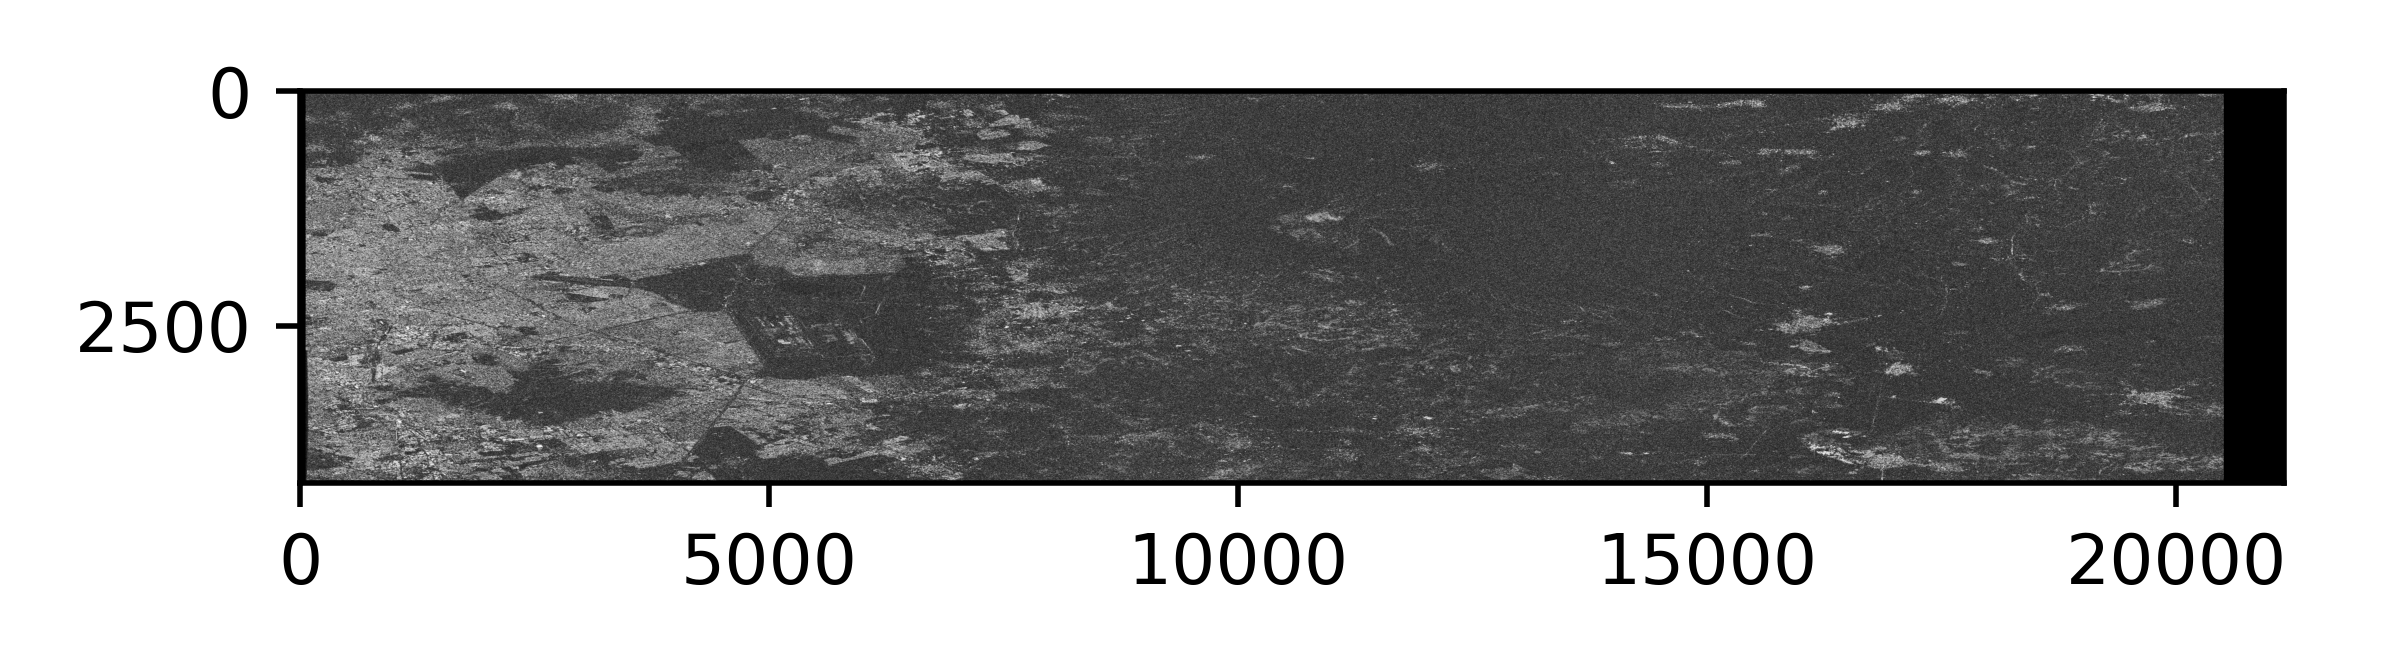
\includegraphics[width=\textwidth]{figure/The coherence/coh_Mexico_asc_esd1.png}
        \end{minipage}%
        \begin{minipage}{0.5\textwidth}
            \centering
            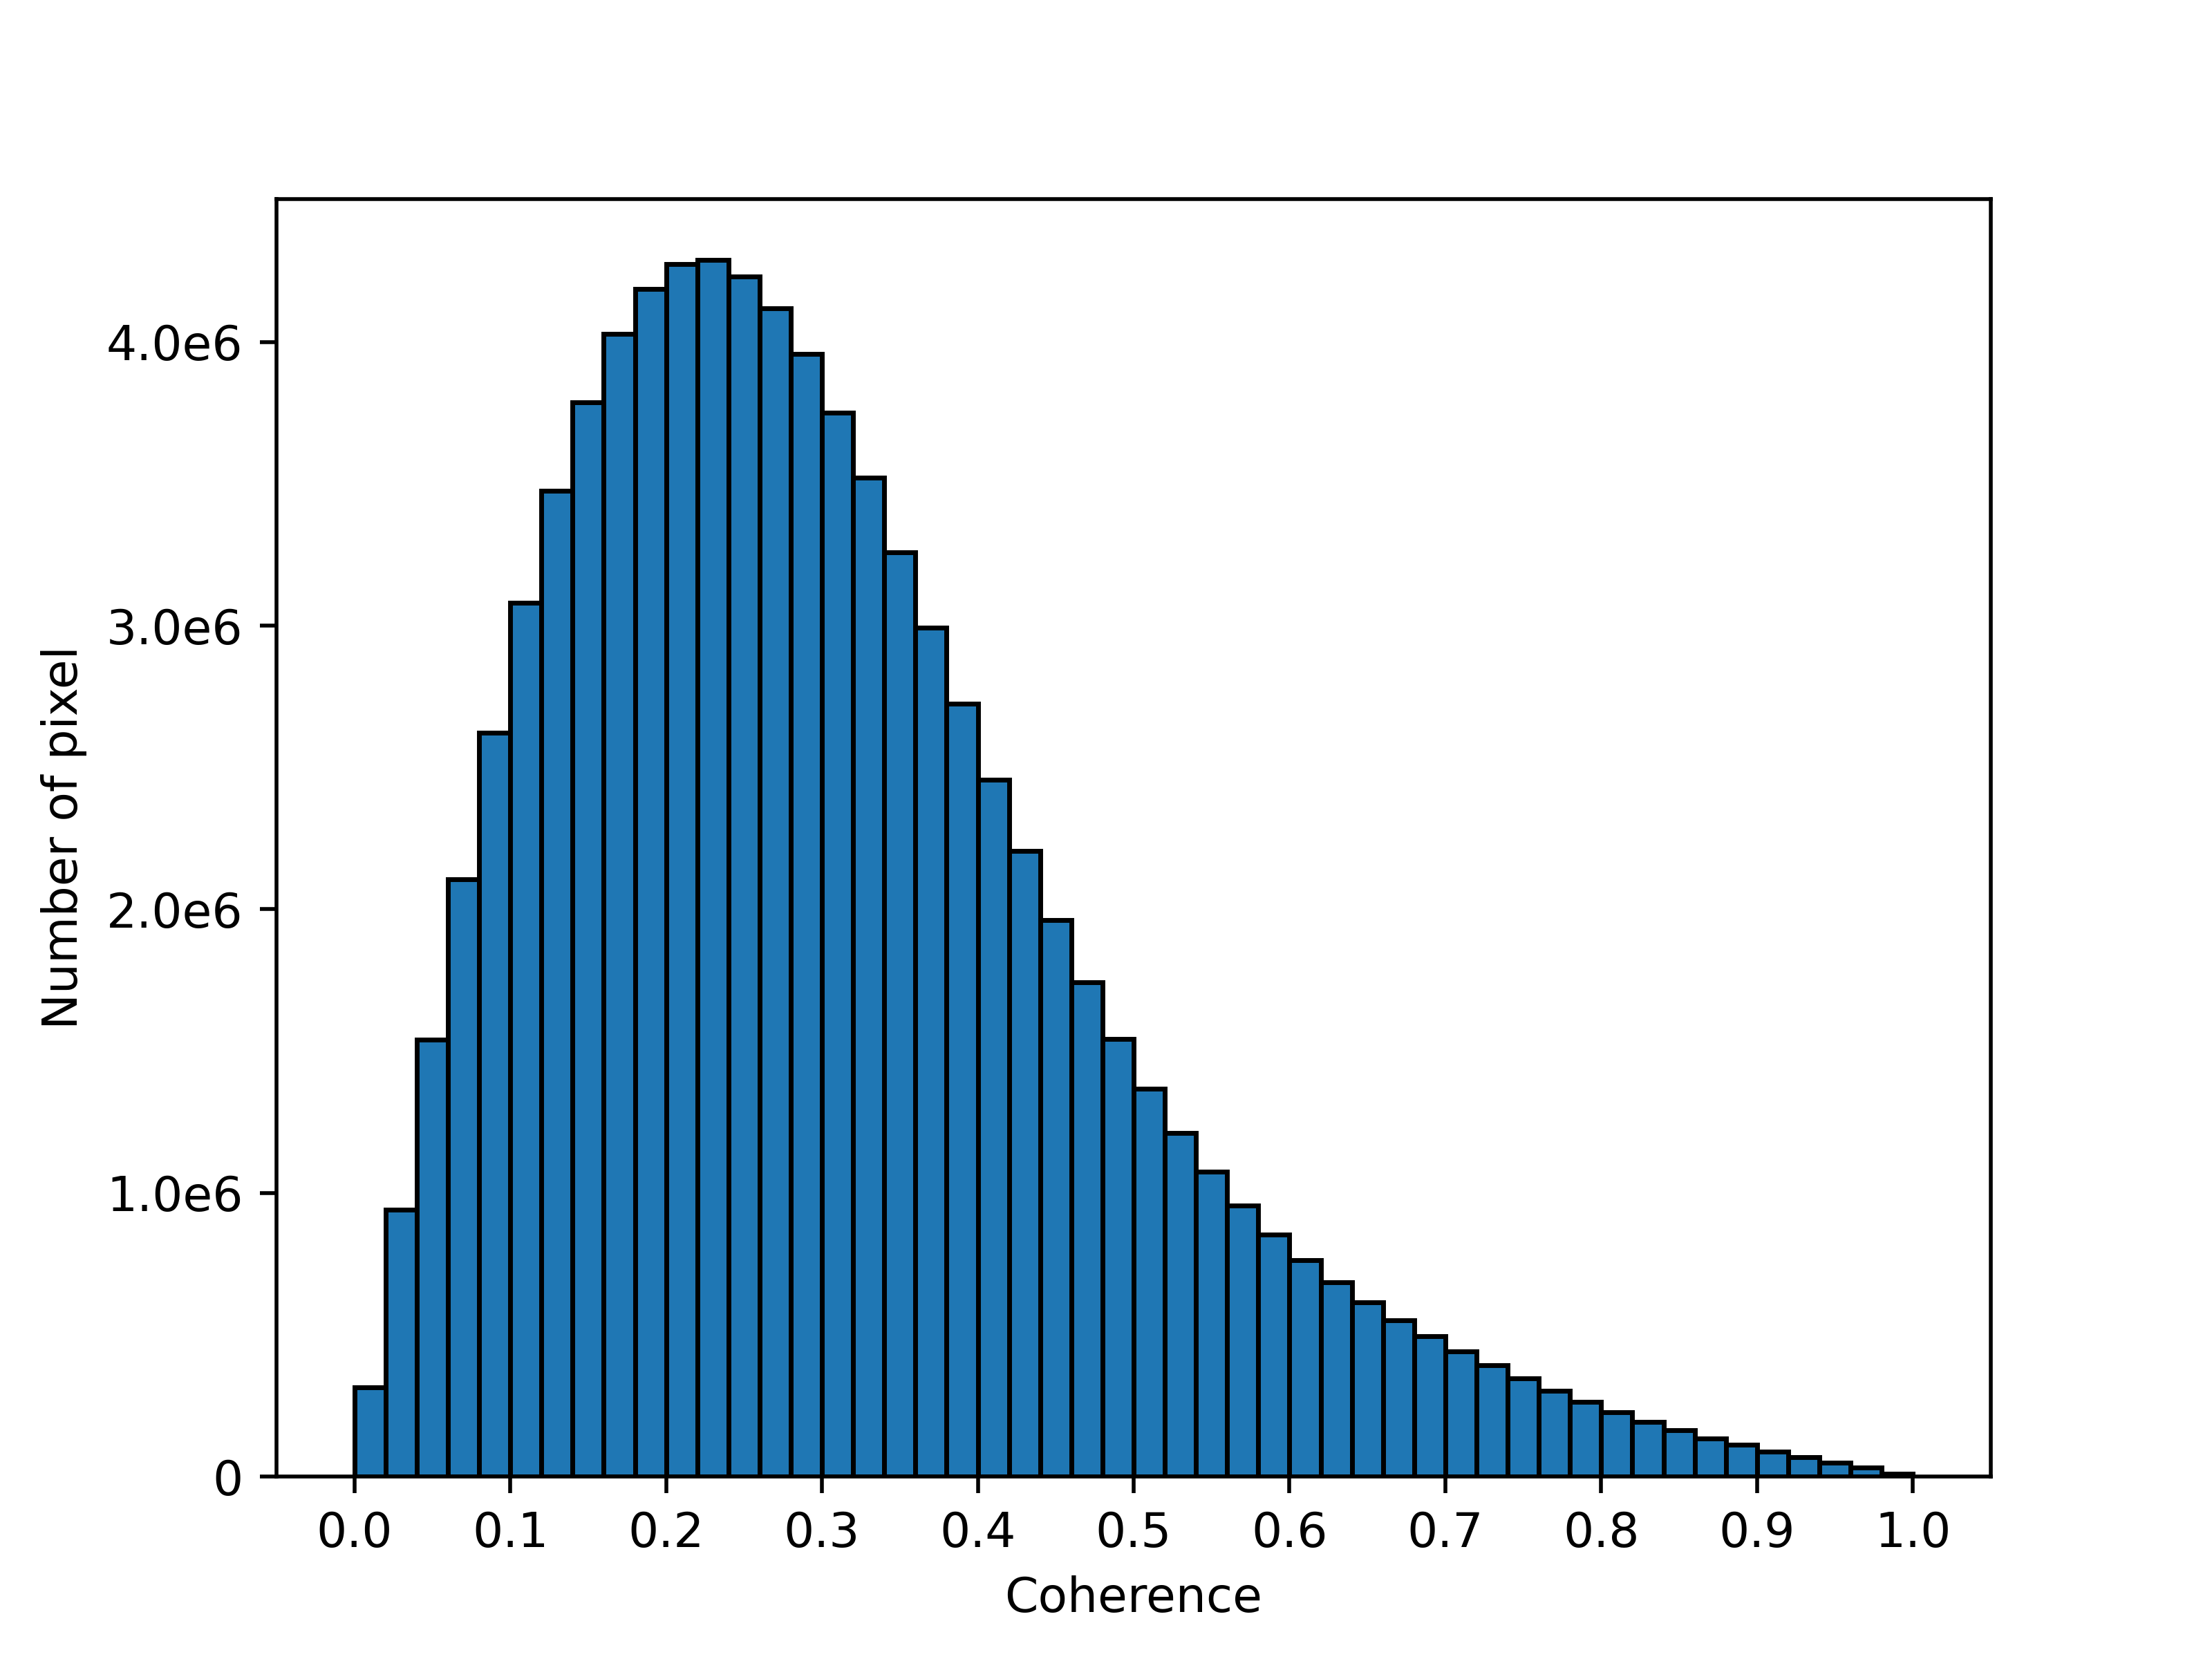
\includegraphics[width=\textwidth]{figure/The coherence/coh_Mexico_asc_esd1_histogram_.png}
        \end{minipage}
        \caption{Mexico City ascending}
        \label{fig_6c}
    \end{subfigure}%
    \begin{subfigure}{0.5\textwidth}
        \centering
        \begin{minipage}{0.5\textwidth}
            \centering
            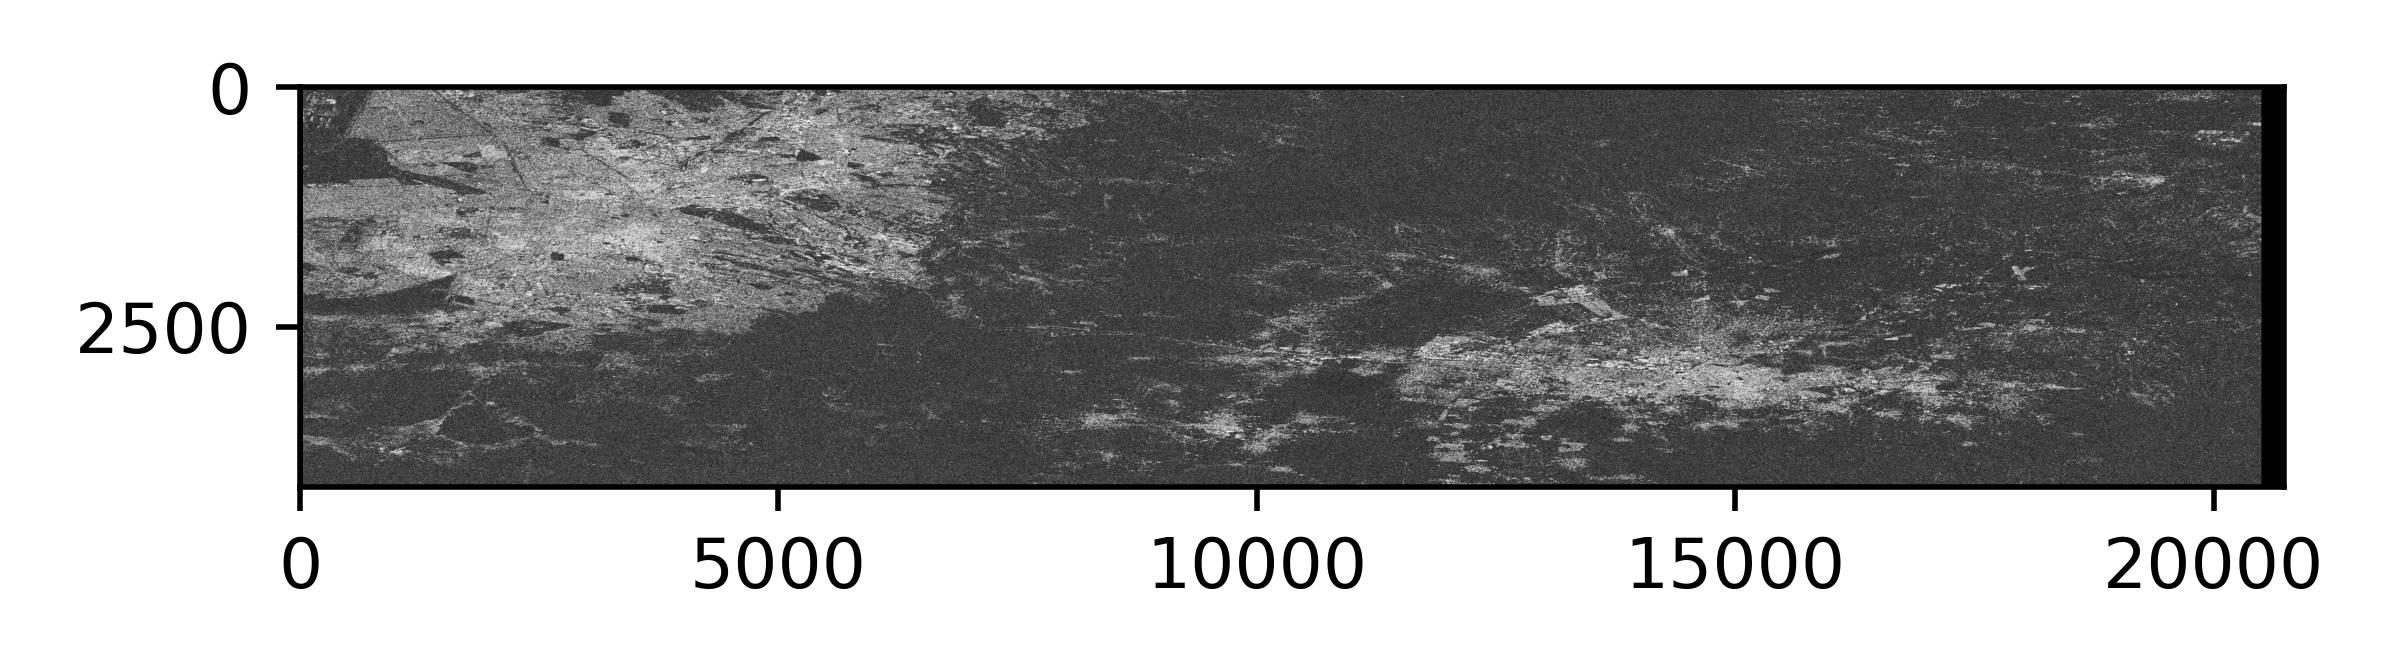
\includegraphics[width=\textwidth]{figure/The coherence/coh_Mexico_des_esd1.png}
        \end{minipage}%
        \begin{minipage}{0.5\textwidth}
            \centering
            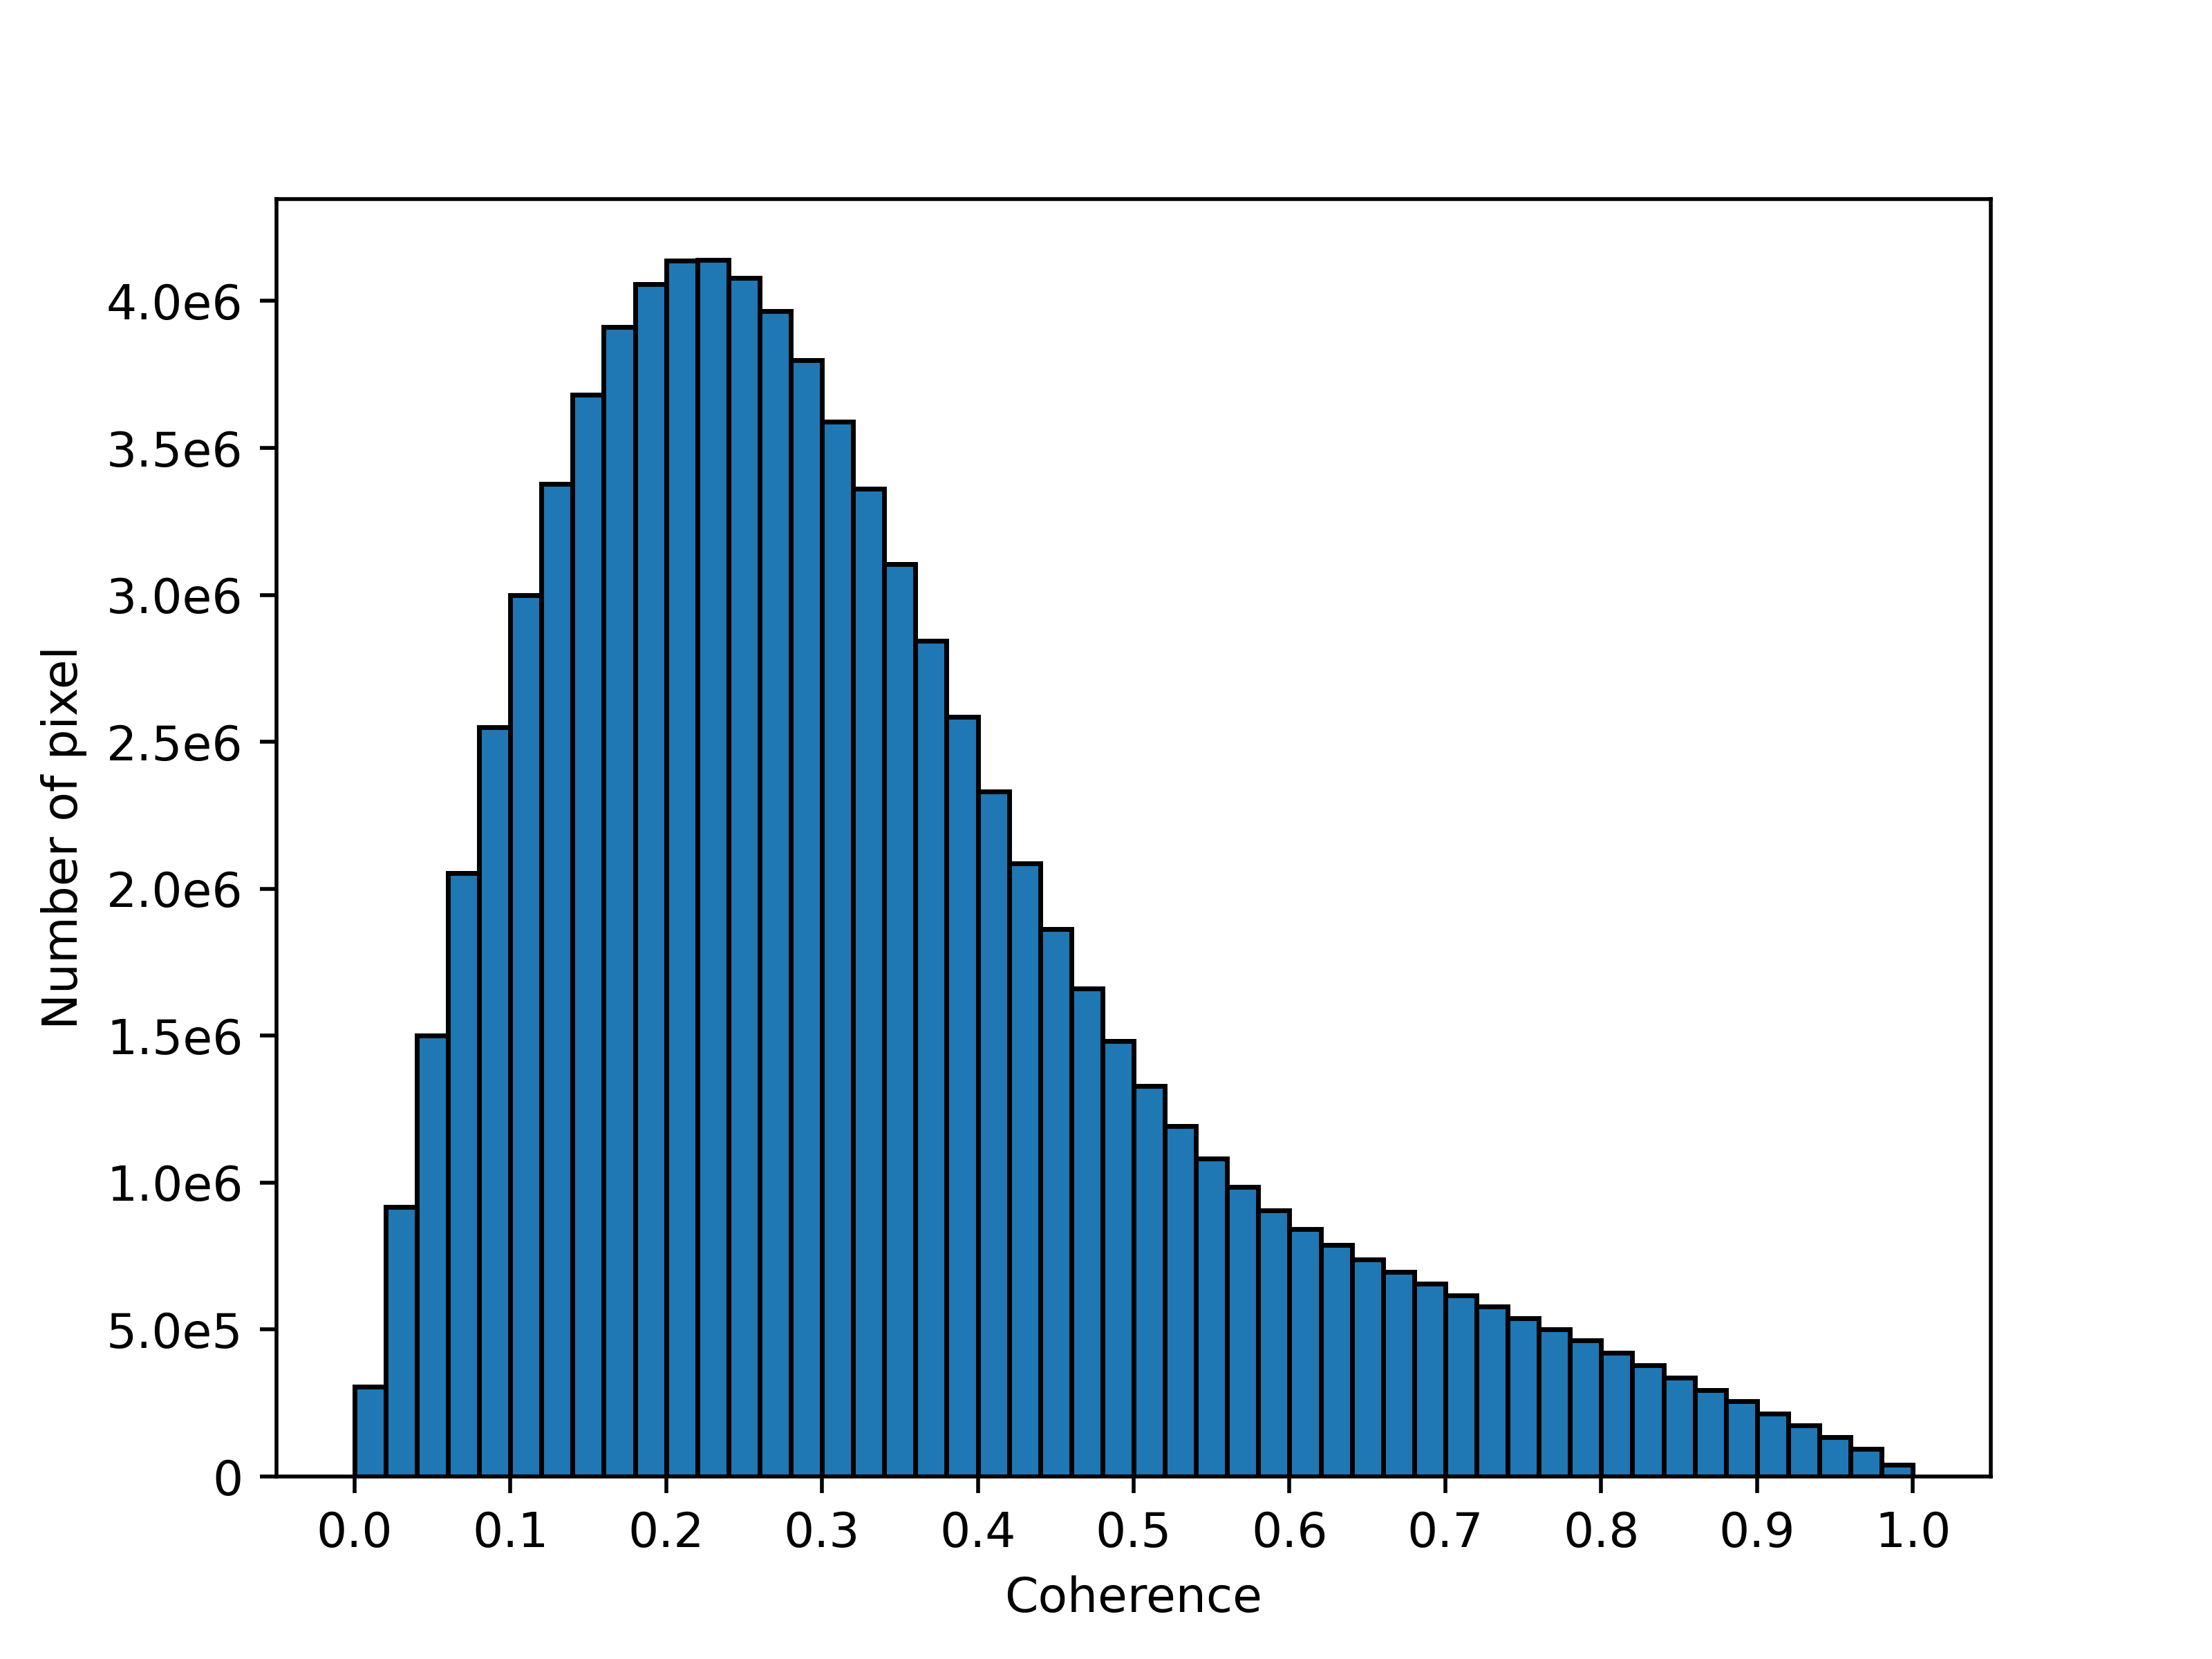
\includegraphics[width=\textwidth]{figure/The coherence/coh_Mexico_des_esd1_histogram_.png}
        \end{minipage}
        \caption{Mexico City descending}
        \label{fig_6d}
    \end{subfigure}%
    \hfill
    \begin{subfigure}{0.5\textwidth}
        \centering
        \begin{minipage}{0.5\textwidth}
            \centering
            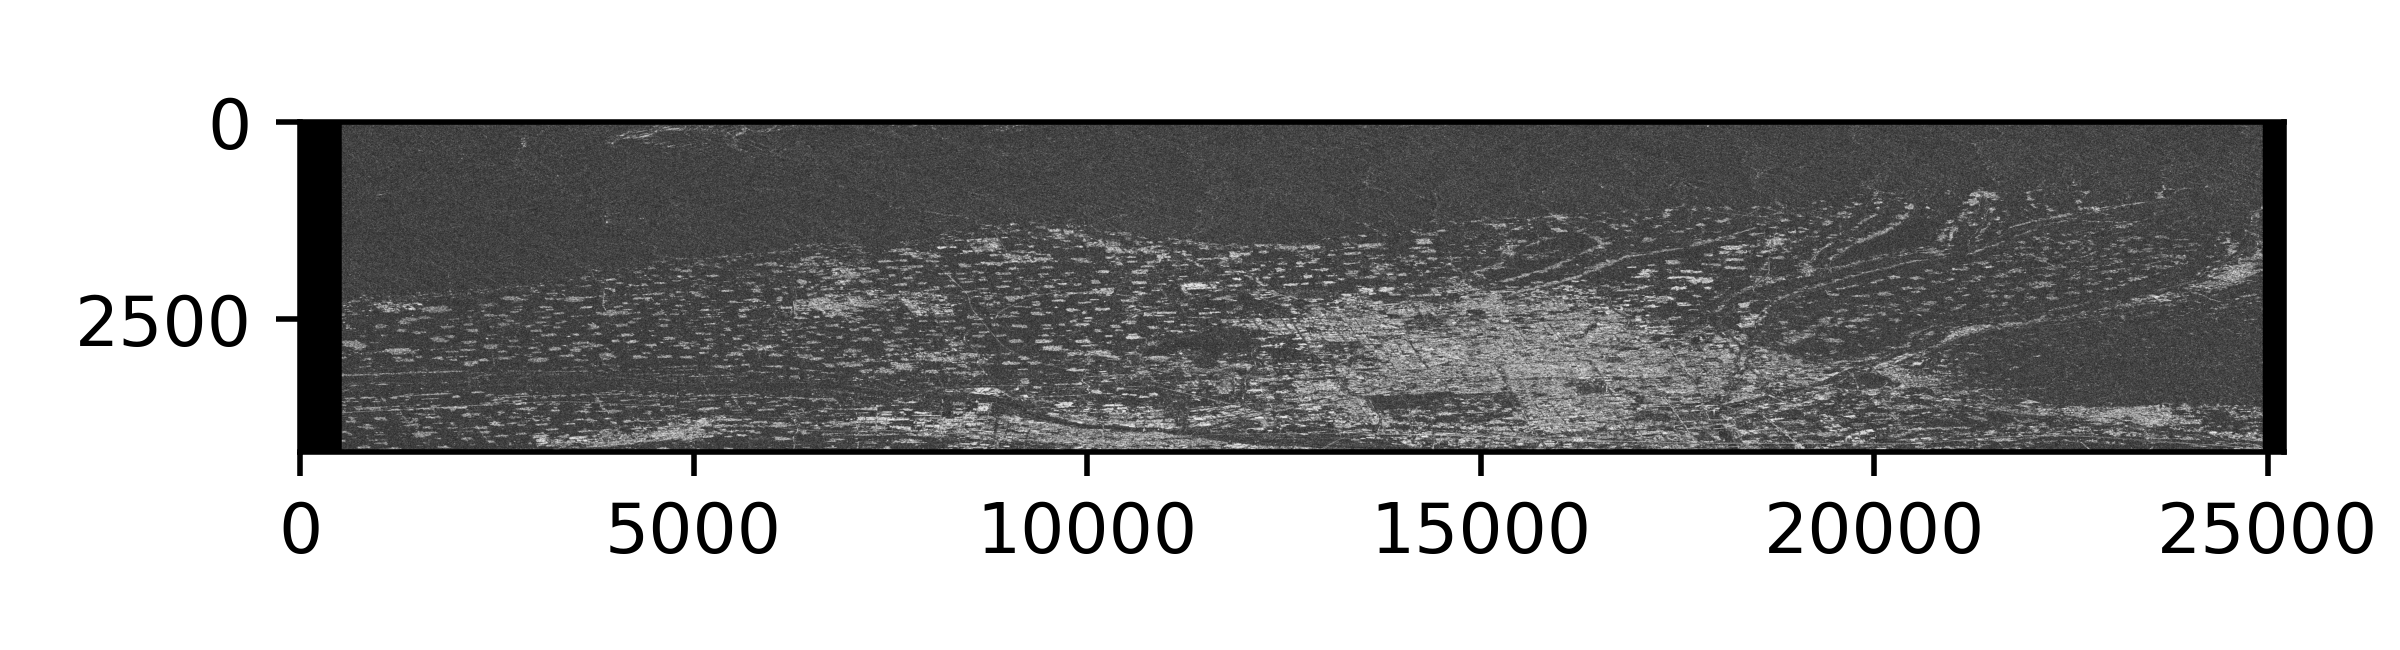
\includegraphics[width=\textwidth]{figure/The coherence/coh_XiAn_asc_esd1.png}
        \end{minipage}%
        \begin{minipage}{0.5\textwidth}
            \centering
            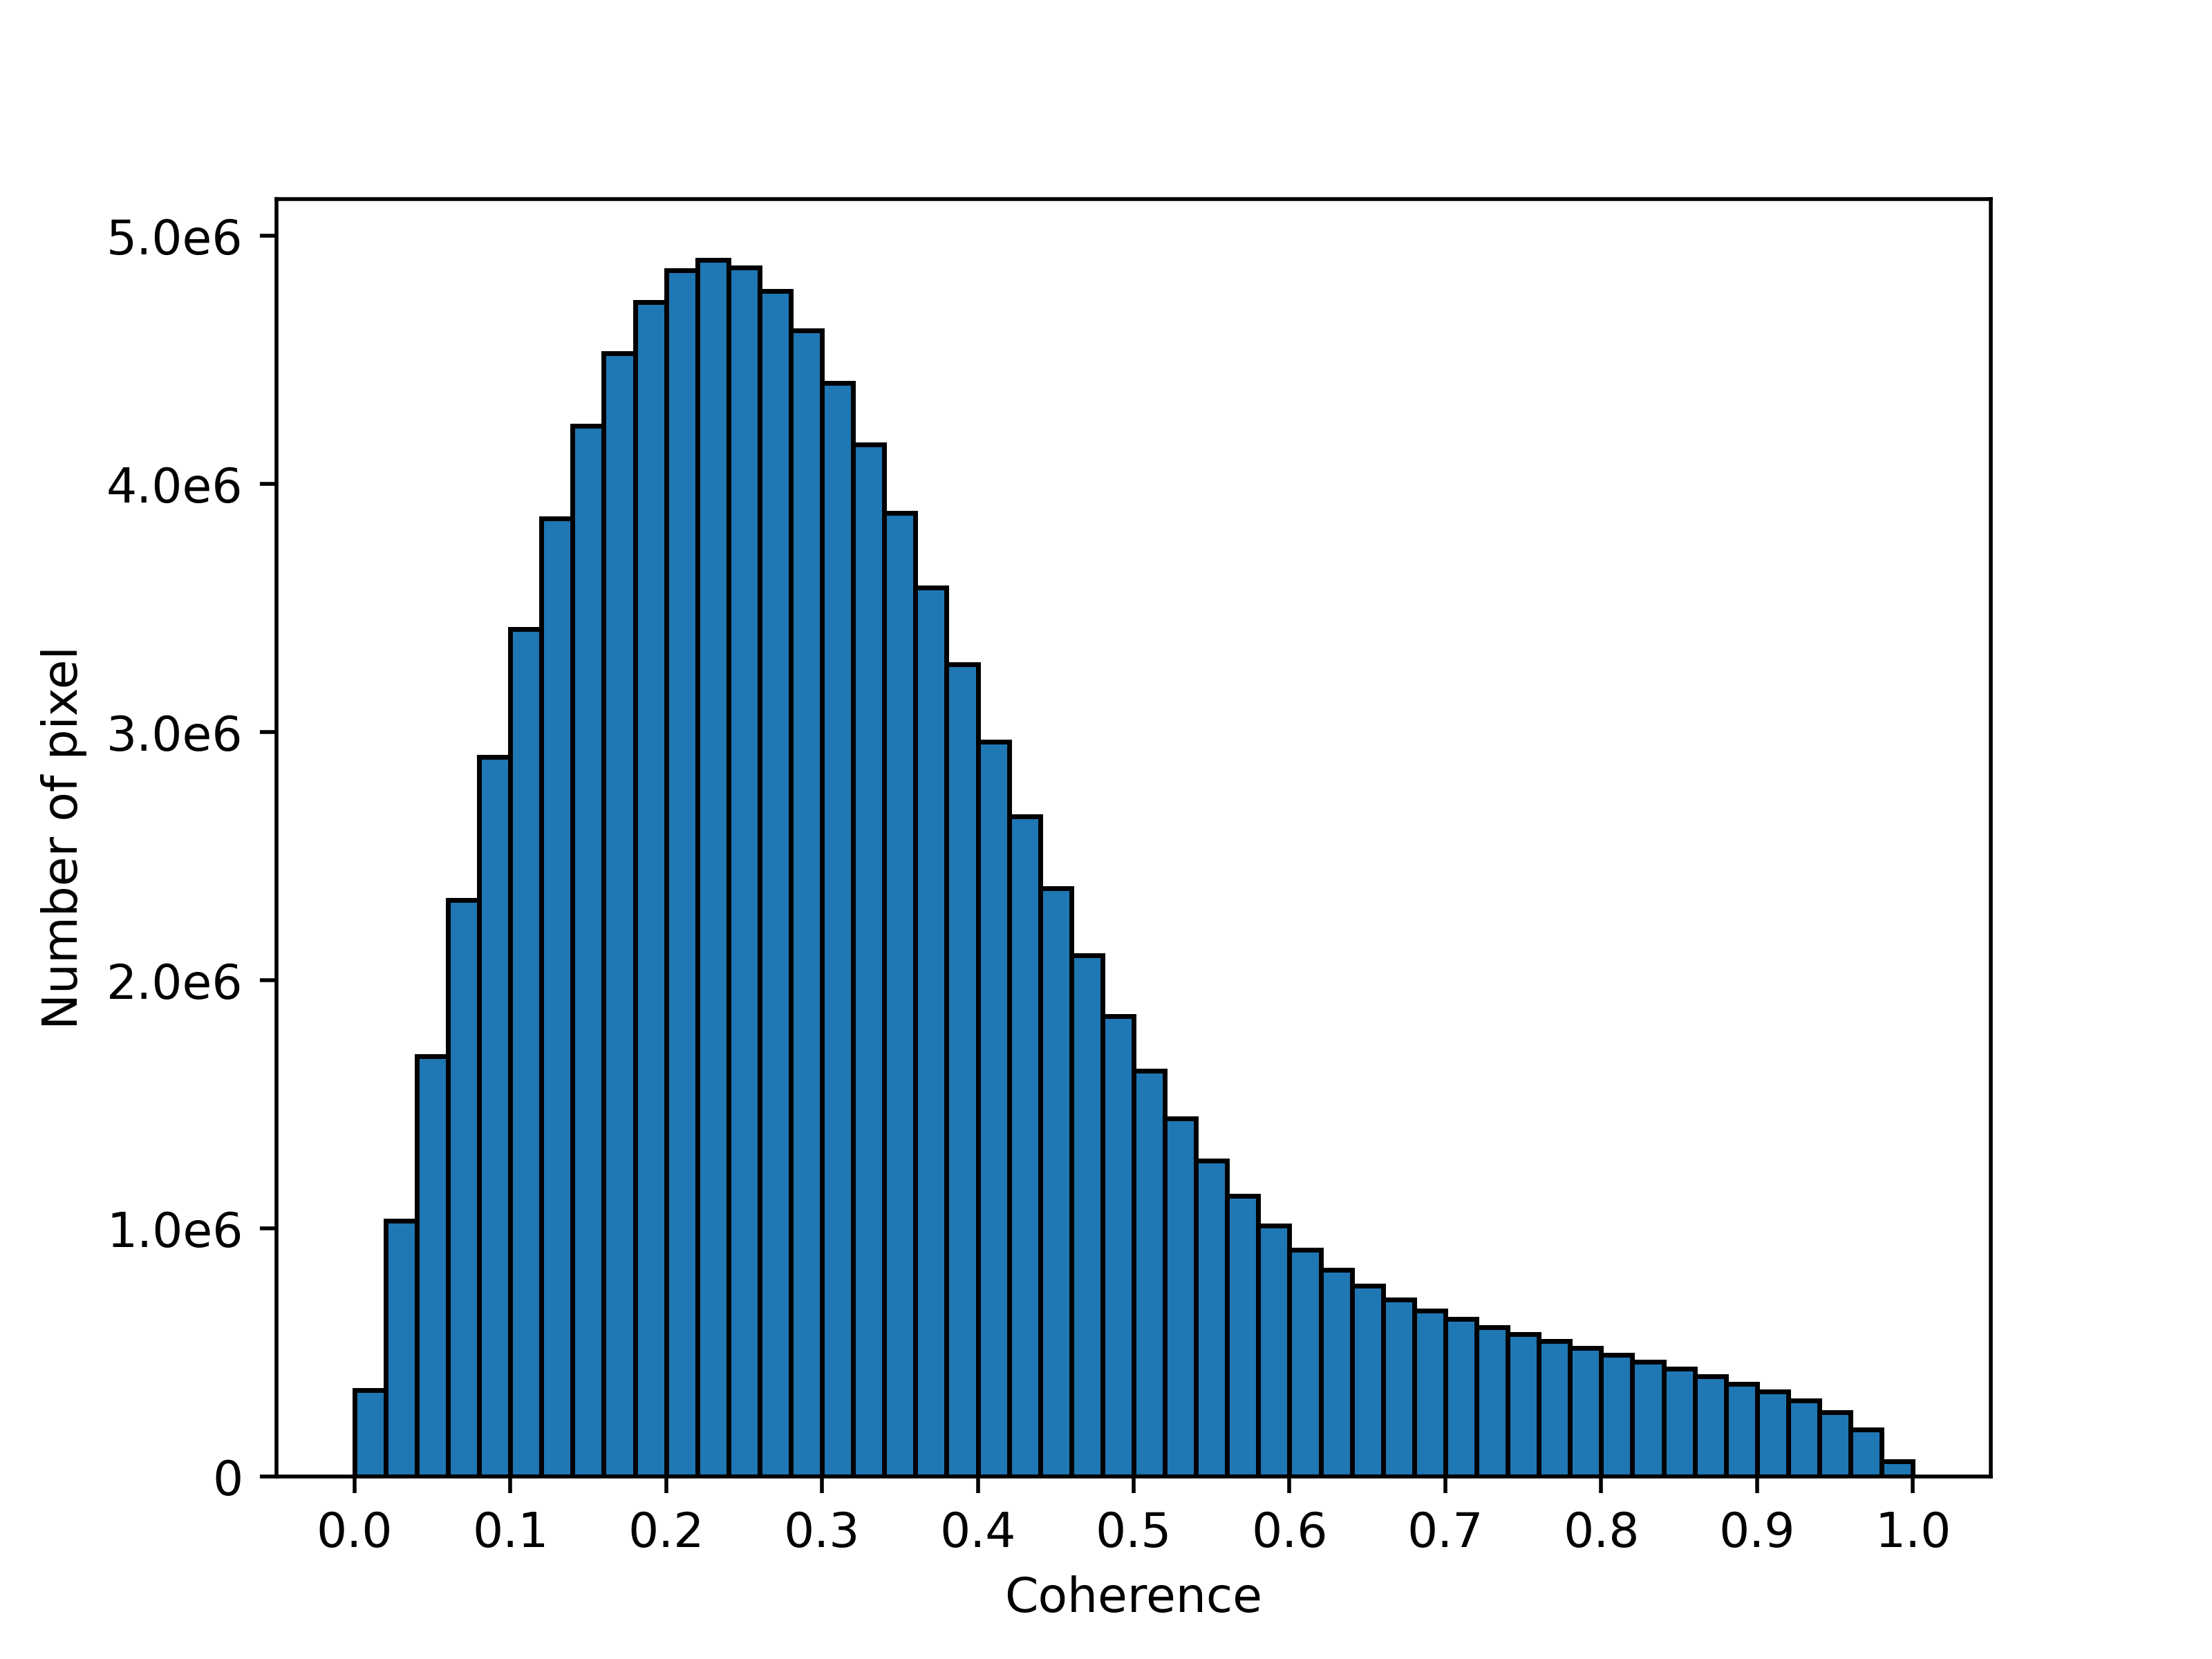
\includegraphics[width=\textwidth]{figure/The coherence/coh_XiAn_asc_esd1_histogram_.png}
        \end{minipage}
        \caption{Xi'an ascending}
        \label{fig_6e}
    \end{subfigure}%
    \begin{subfigure}{0.5\textwidth}
        \centering
        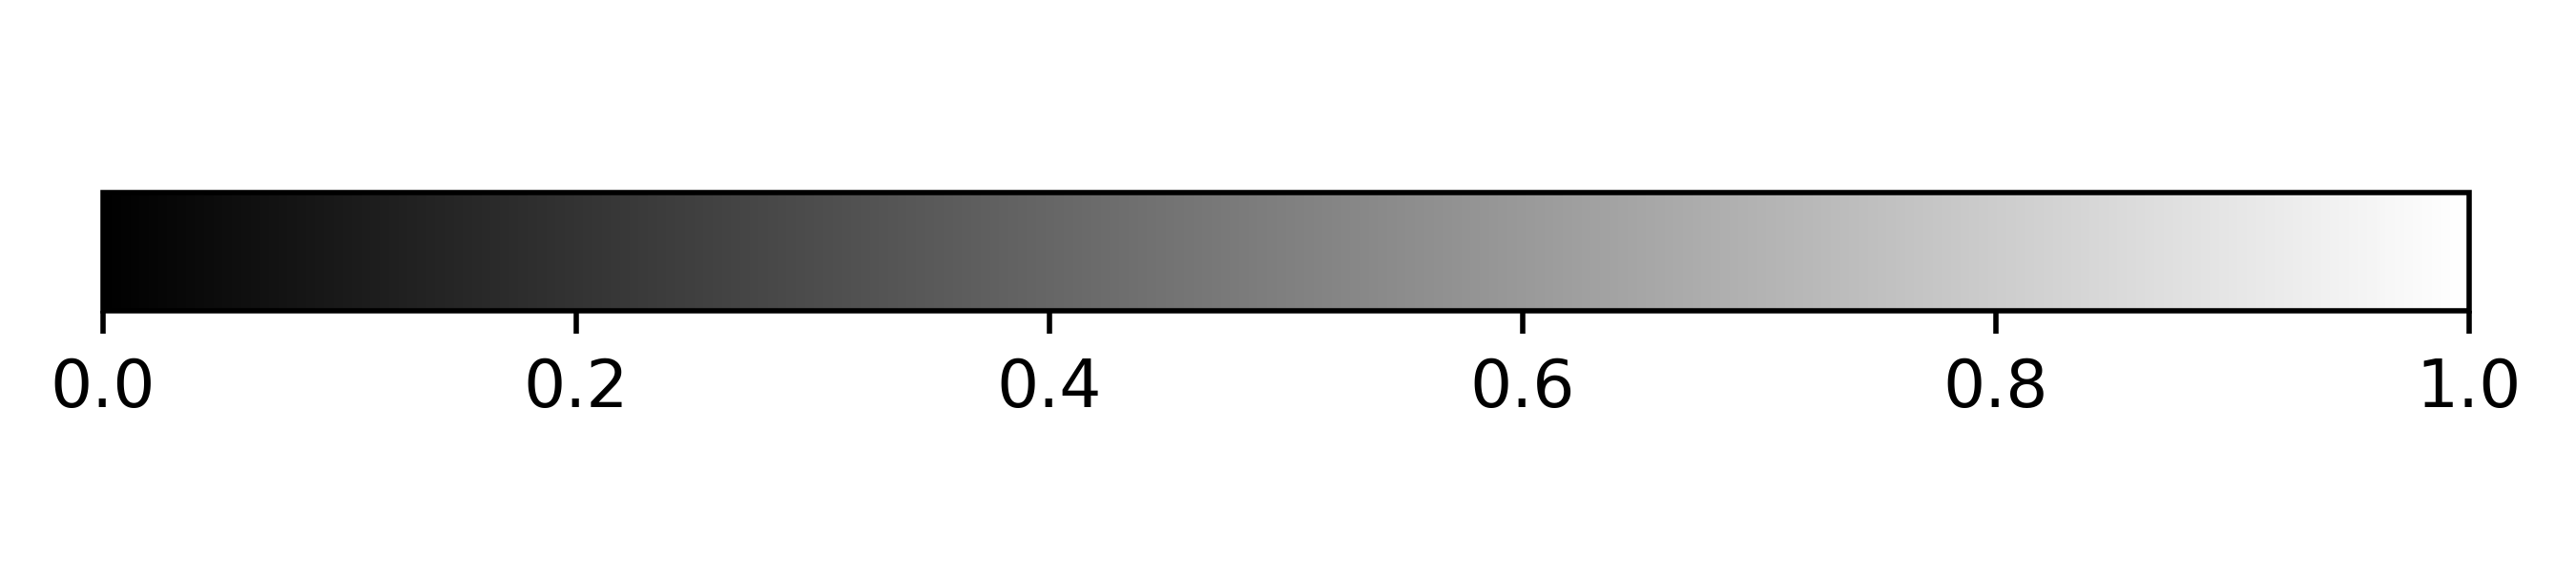
\includegraphics[width=\textwidth]{figure/The coherence/colorbar.png}
        \caption*{}
    \end{subfigure}%
    \hfill
    \begin{subfigure}{0.5\textwidth}
        \centering
        \begin{minipage}{0.5\textwidth}
            \centering
            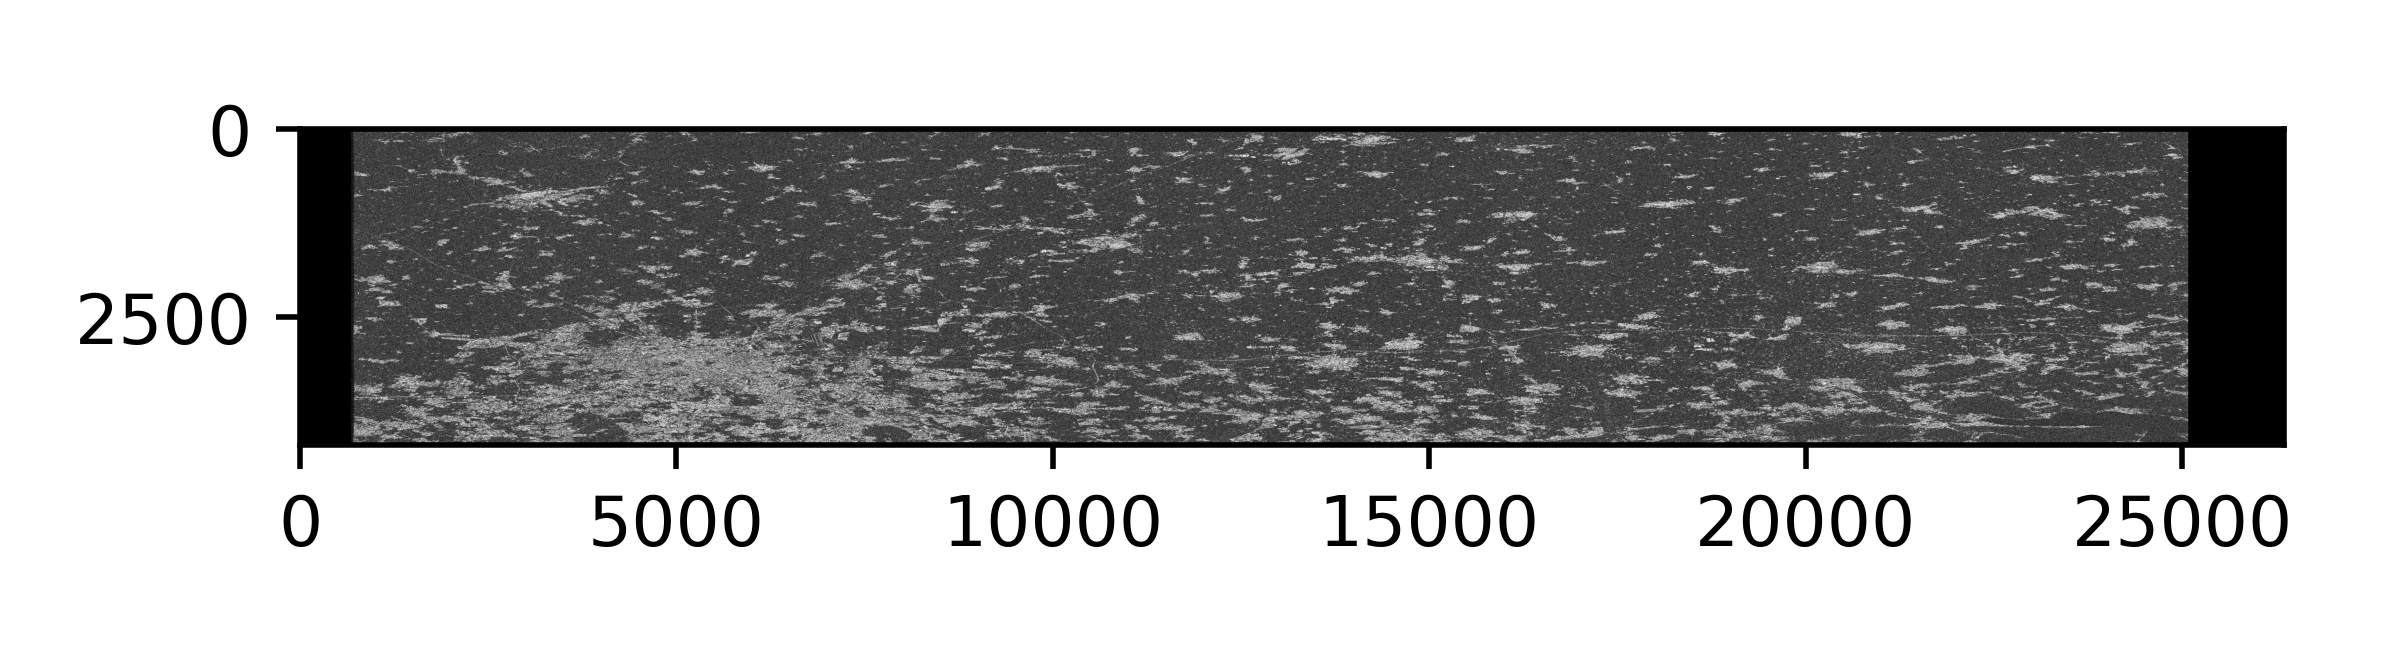
\includegraphics[width=\textwidth]{figure/The coherence/coh_Milan_asc_esd1.png}
        \end{minipage}%
        \begin{minipage}{0.5\textwidth}
            \centering
            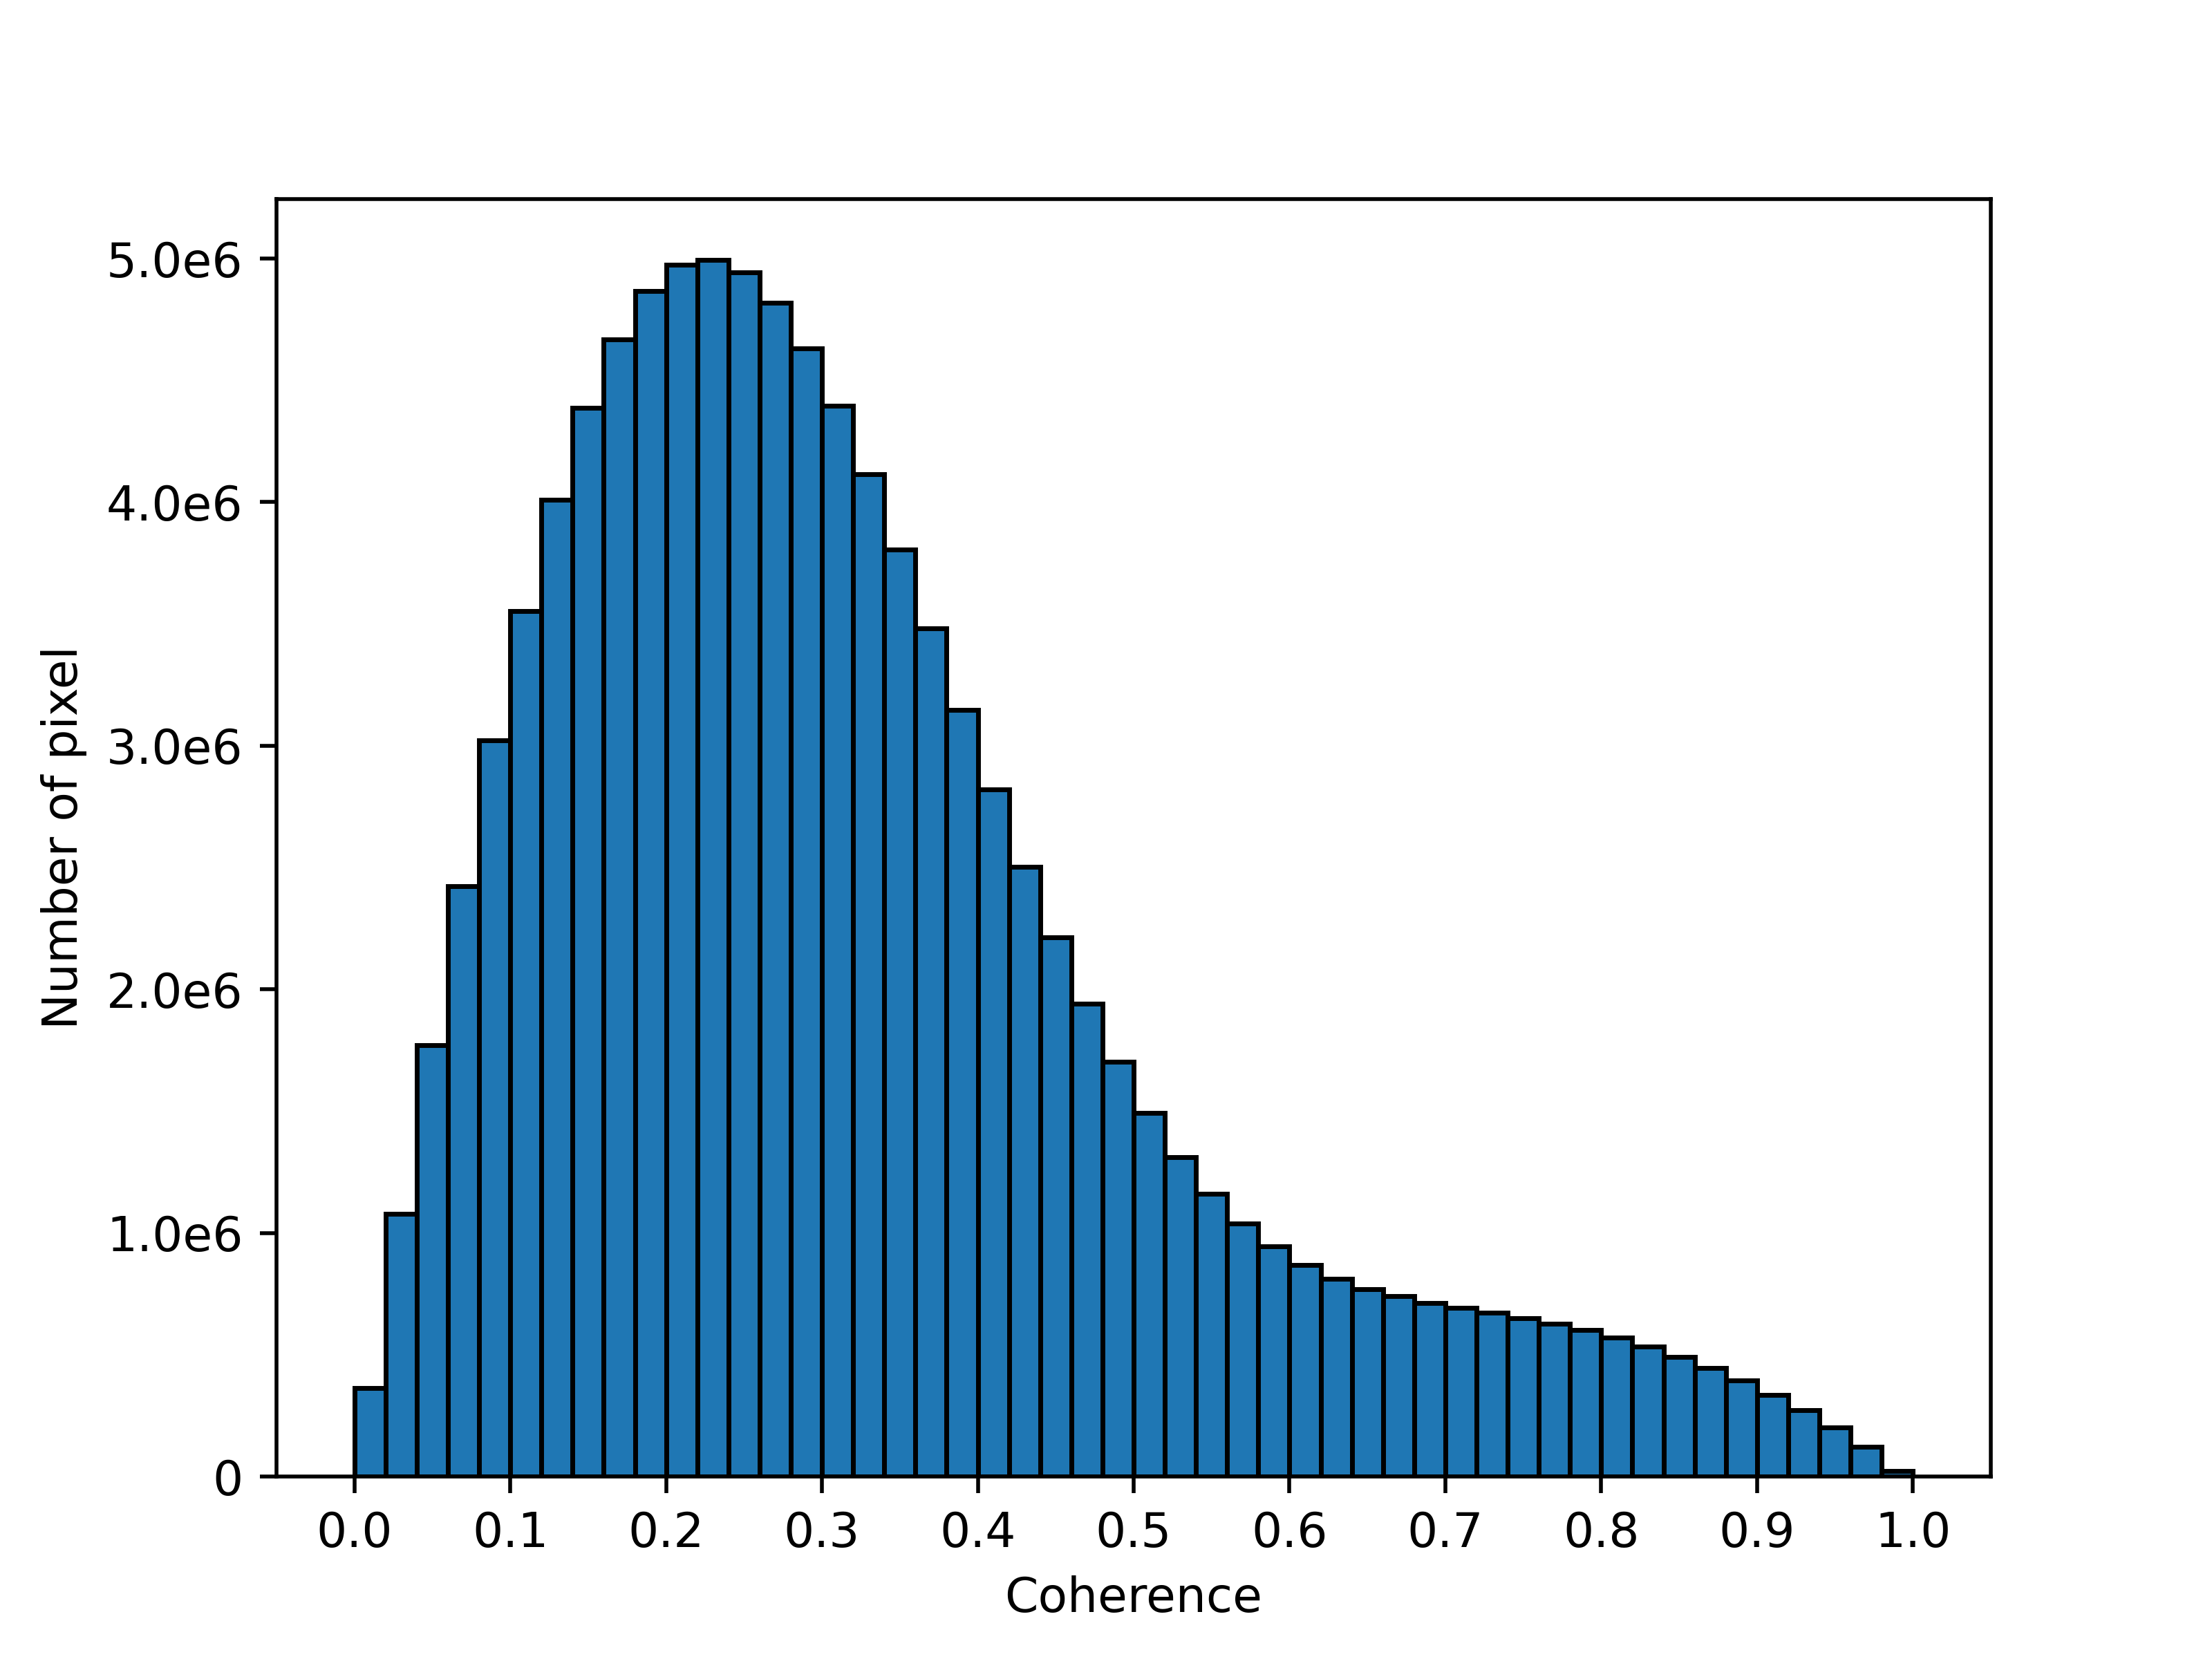
\includegraphics[width=\textwidth]{figure/The coherence/coh_Milan_asc_esd1_histogram_.png}
        \end{minipage}
        \caption{Milan ascending}
        \label{fig_6f}
    \end{subfigure}%
    \begin{subfigure}{0.5\textwidth}
        \centering
        \begin{minipage}{0.5\textwidth}
            \centering
            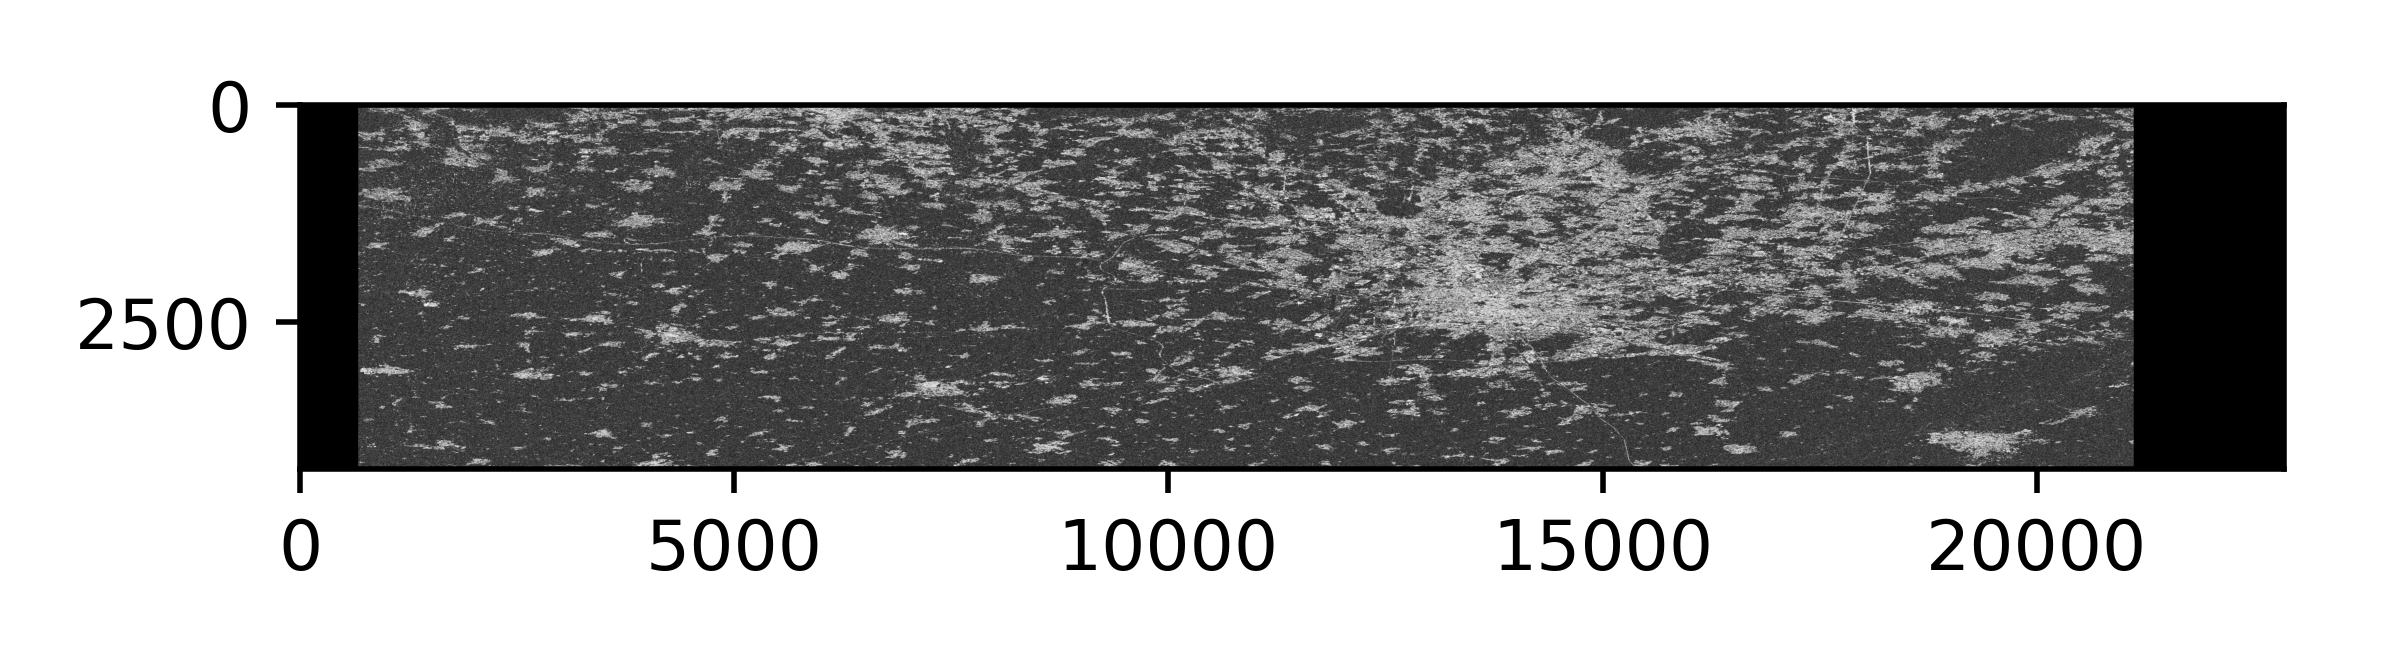
\includegraphics[width=\textwidth]{figure/The coherence/coh_Milan_des_esd1.png}
        \end{minipage}%
        \begin{minipage}{0.5\textwidth}
            \centering
            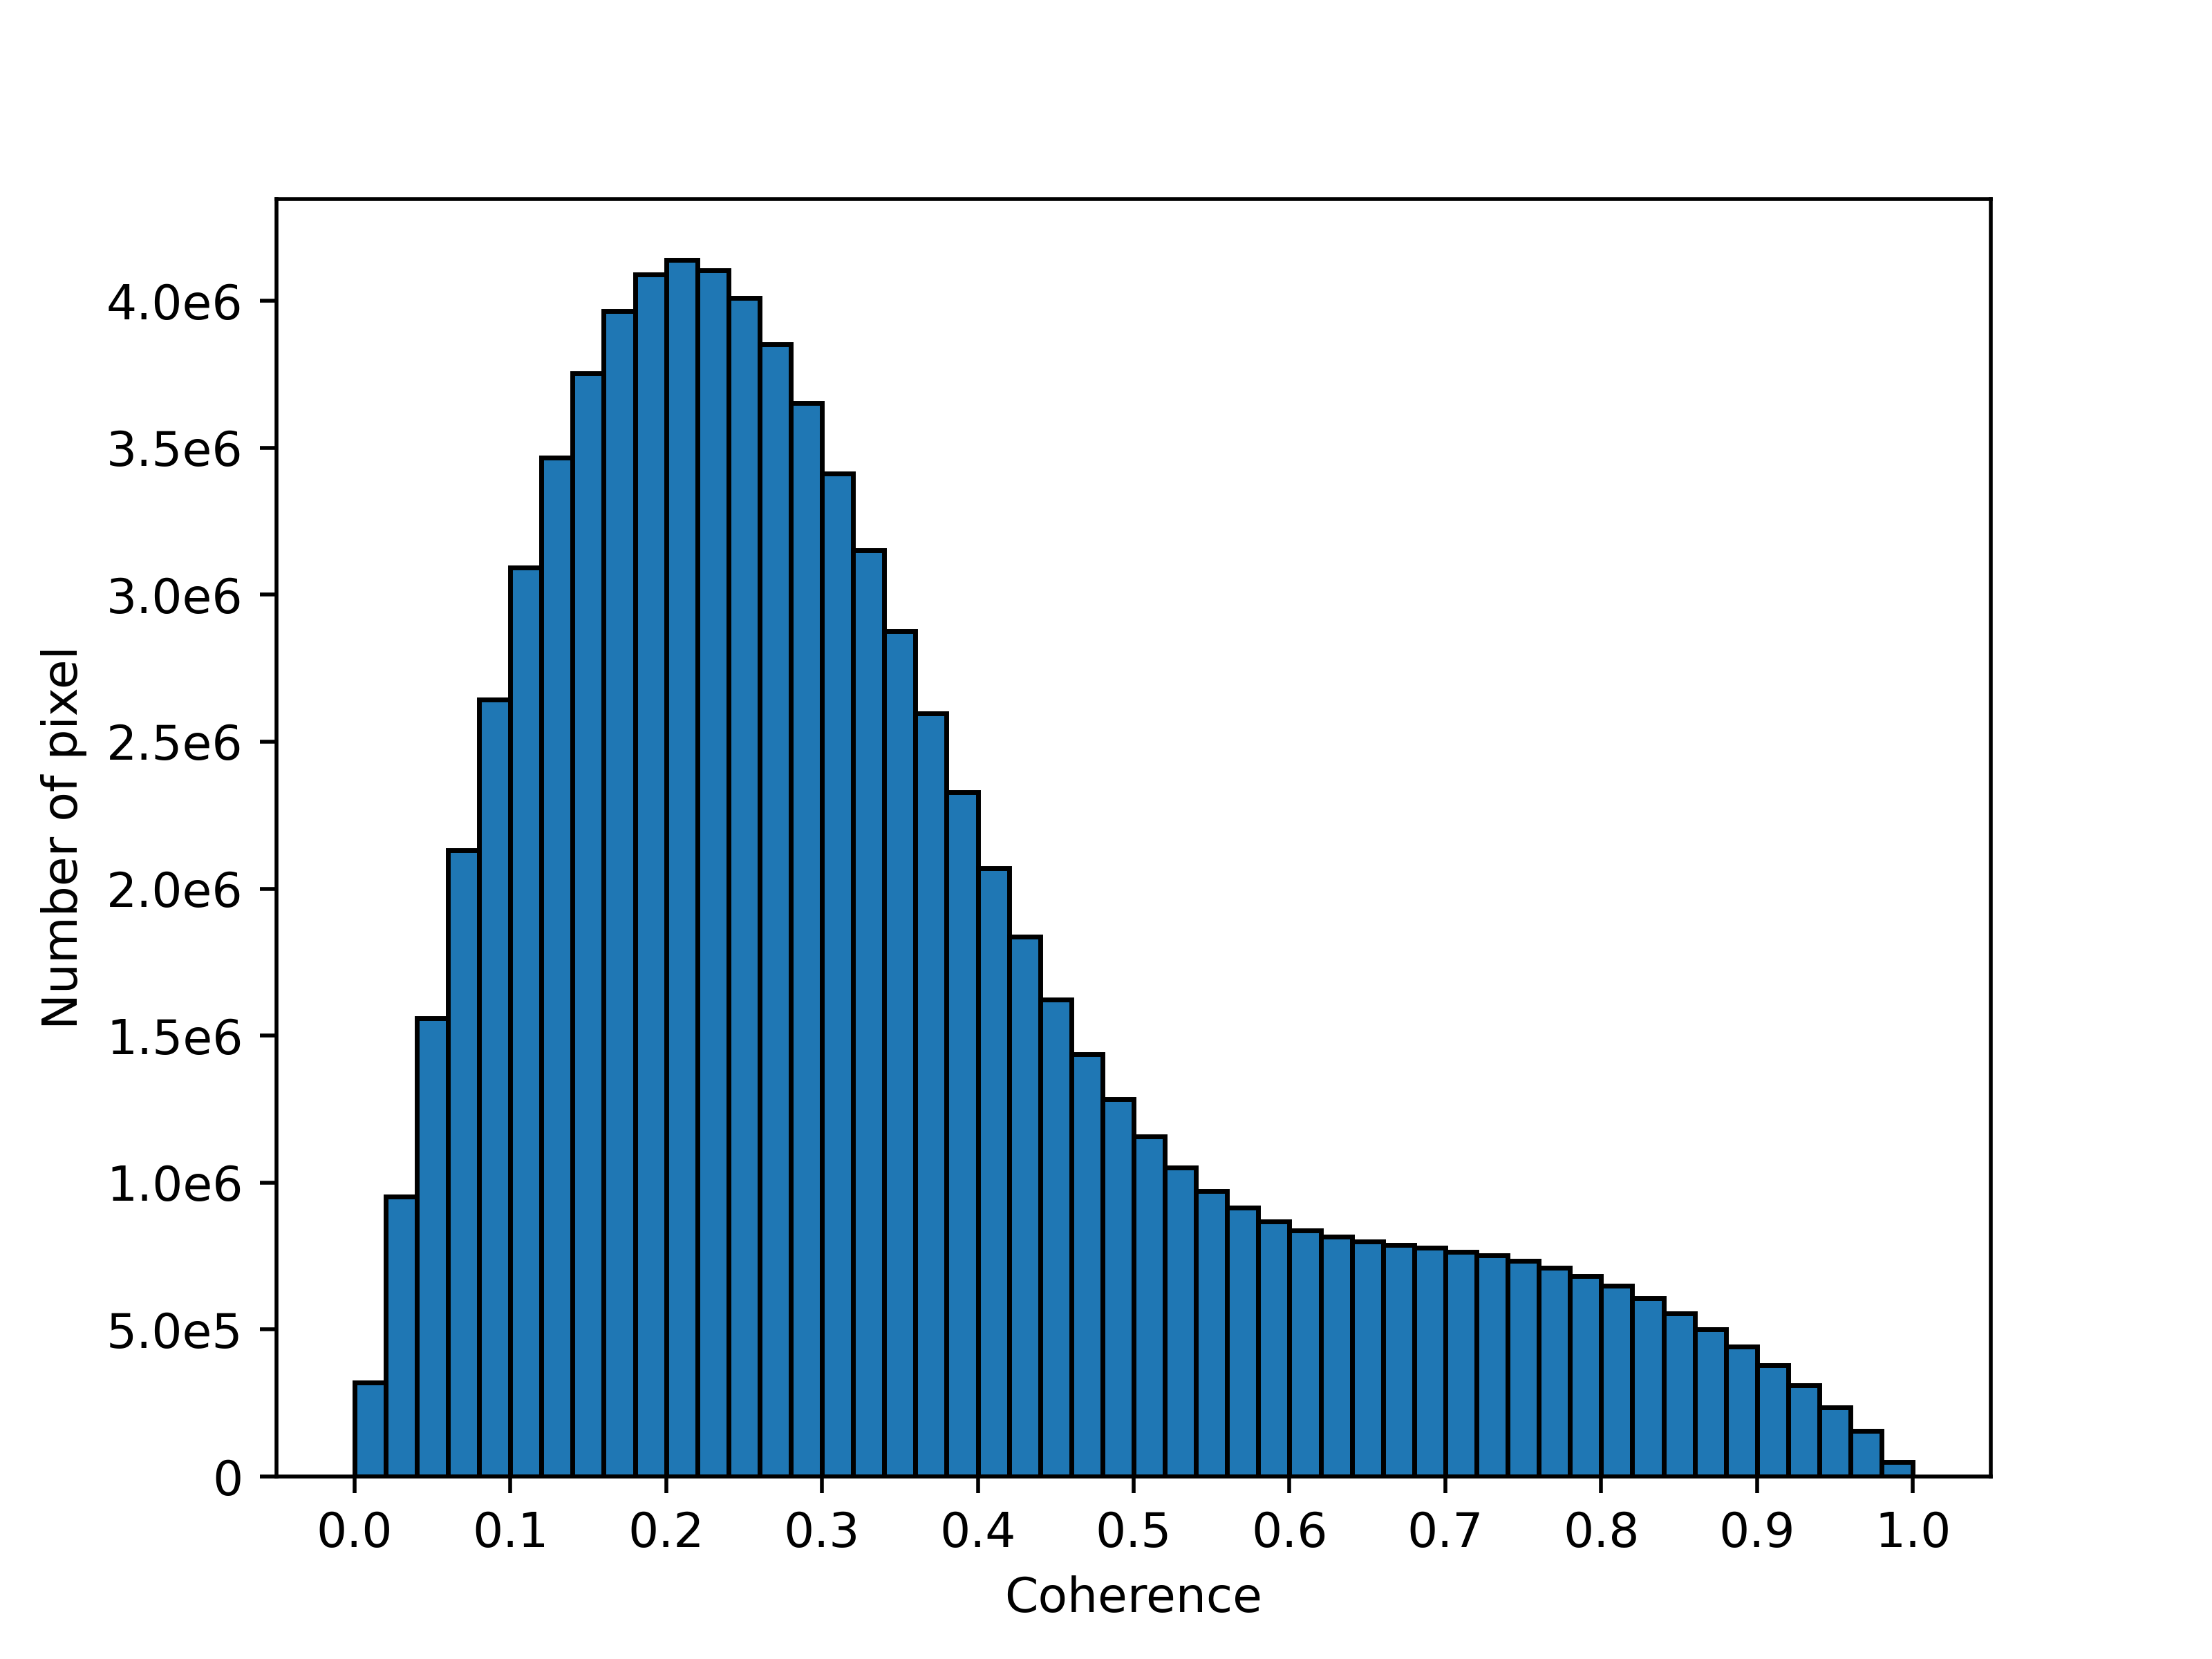
\includegraphics[width=\textwidth]{figure/The coherence/coh_Milan_des_esd1_histogram_.png}
        \end{minipage}
        \caption{Milan descending}
        \label{fig_6g}
    \end{subfigure}%
    \hfill
    \begin{subfigure}{0.5\textwidth}
        \centering
        \begin{minipage}{0.5\textwidth}
            \centering
            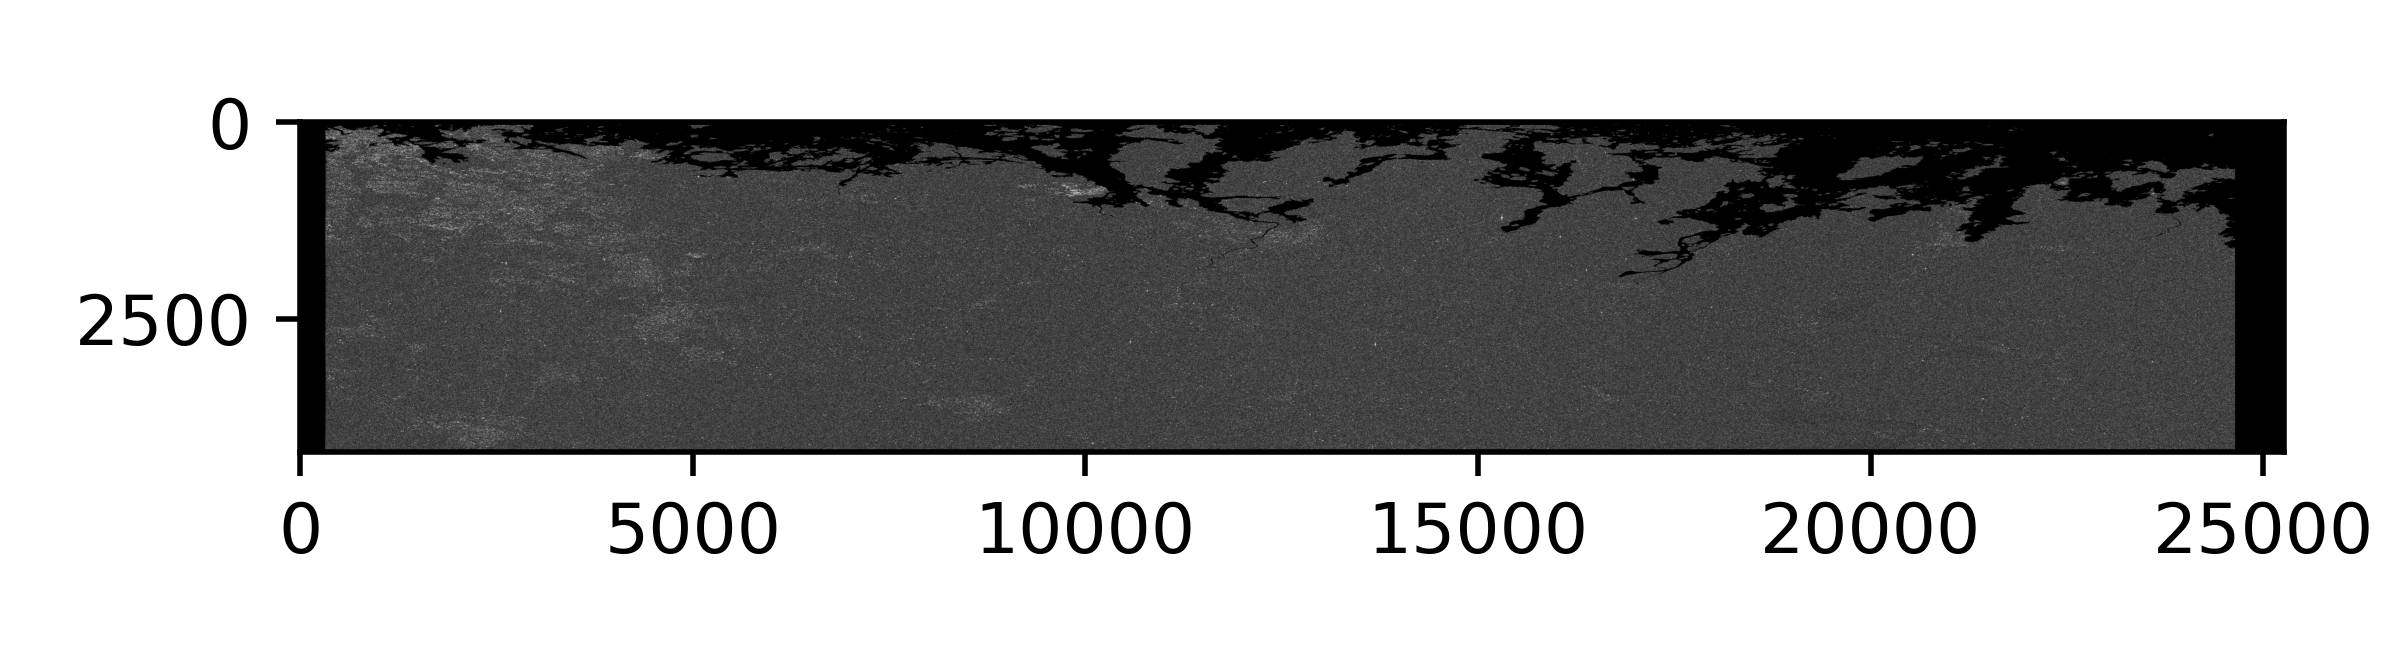
\includegraphics[width=\textwidth]{figure/The coherence/coh_Finland_asc_esd1.png}
        \end{minipage}%
        \begin{minipage}{0.5\textwidth}
            \centering
            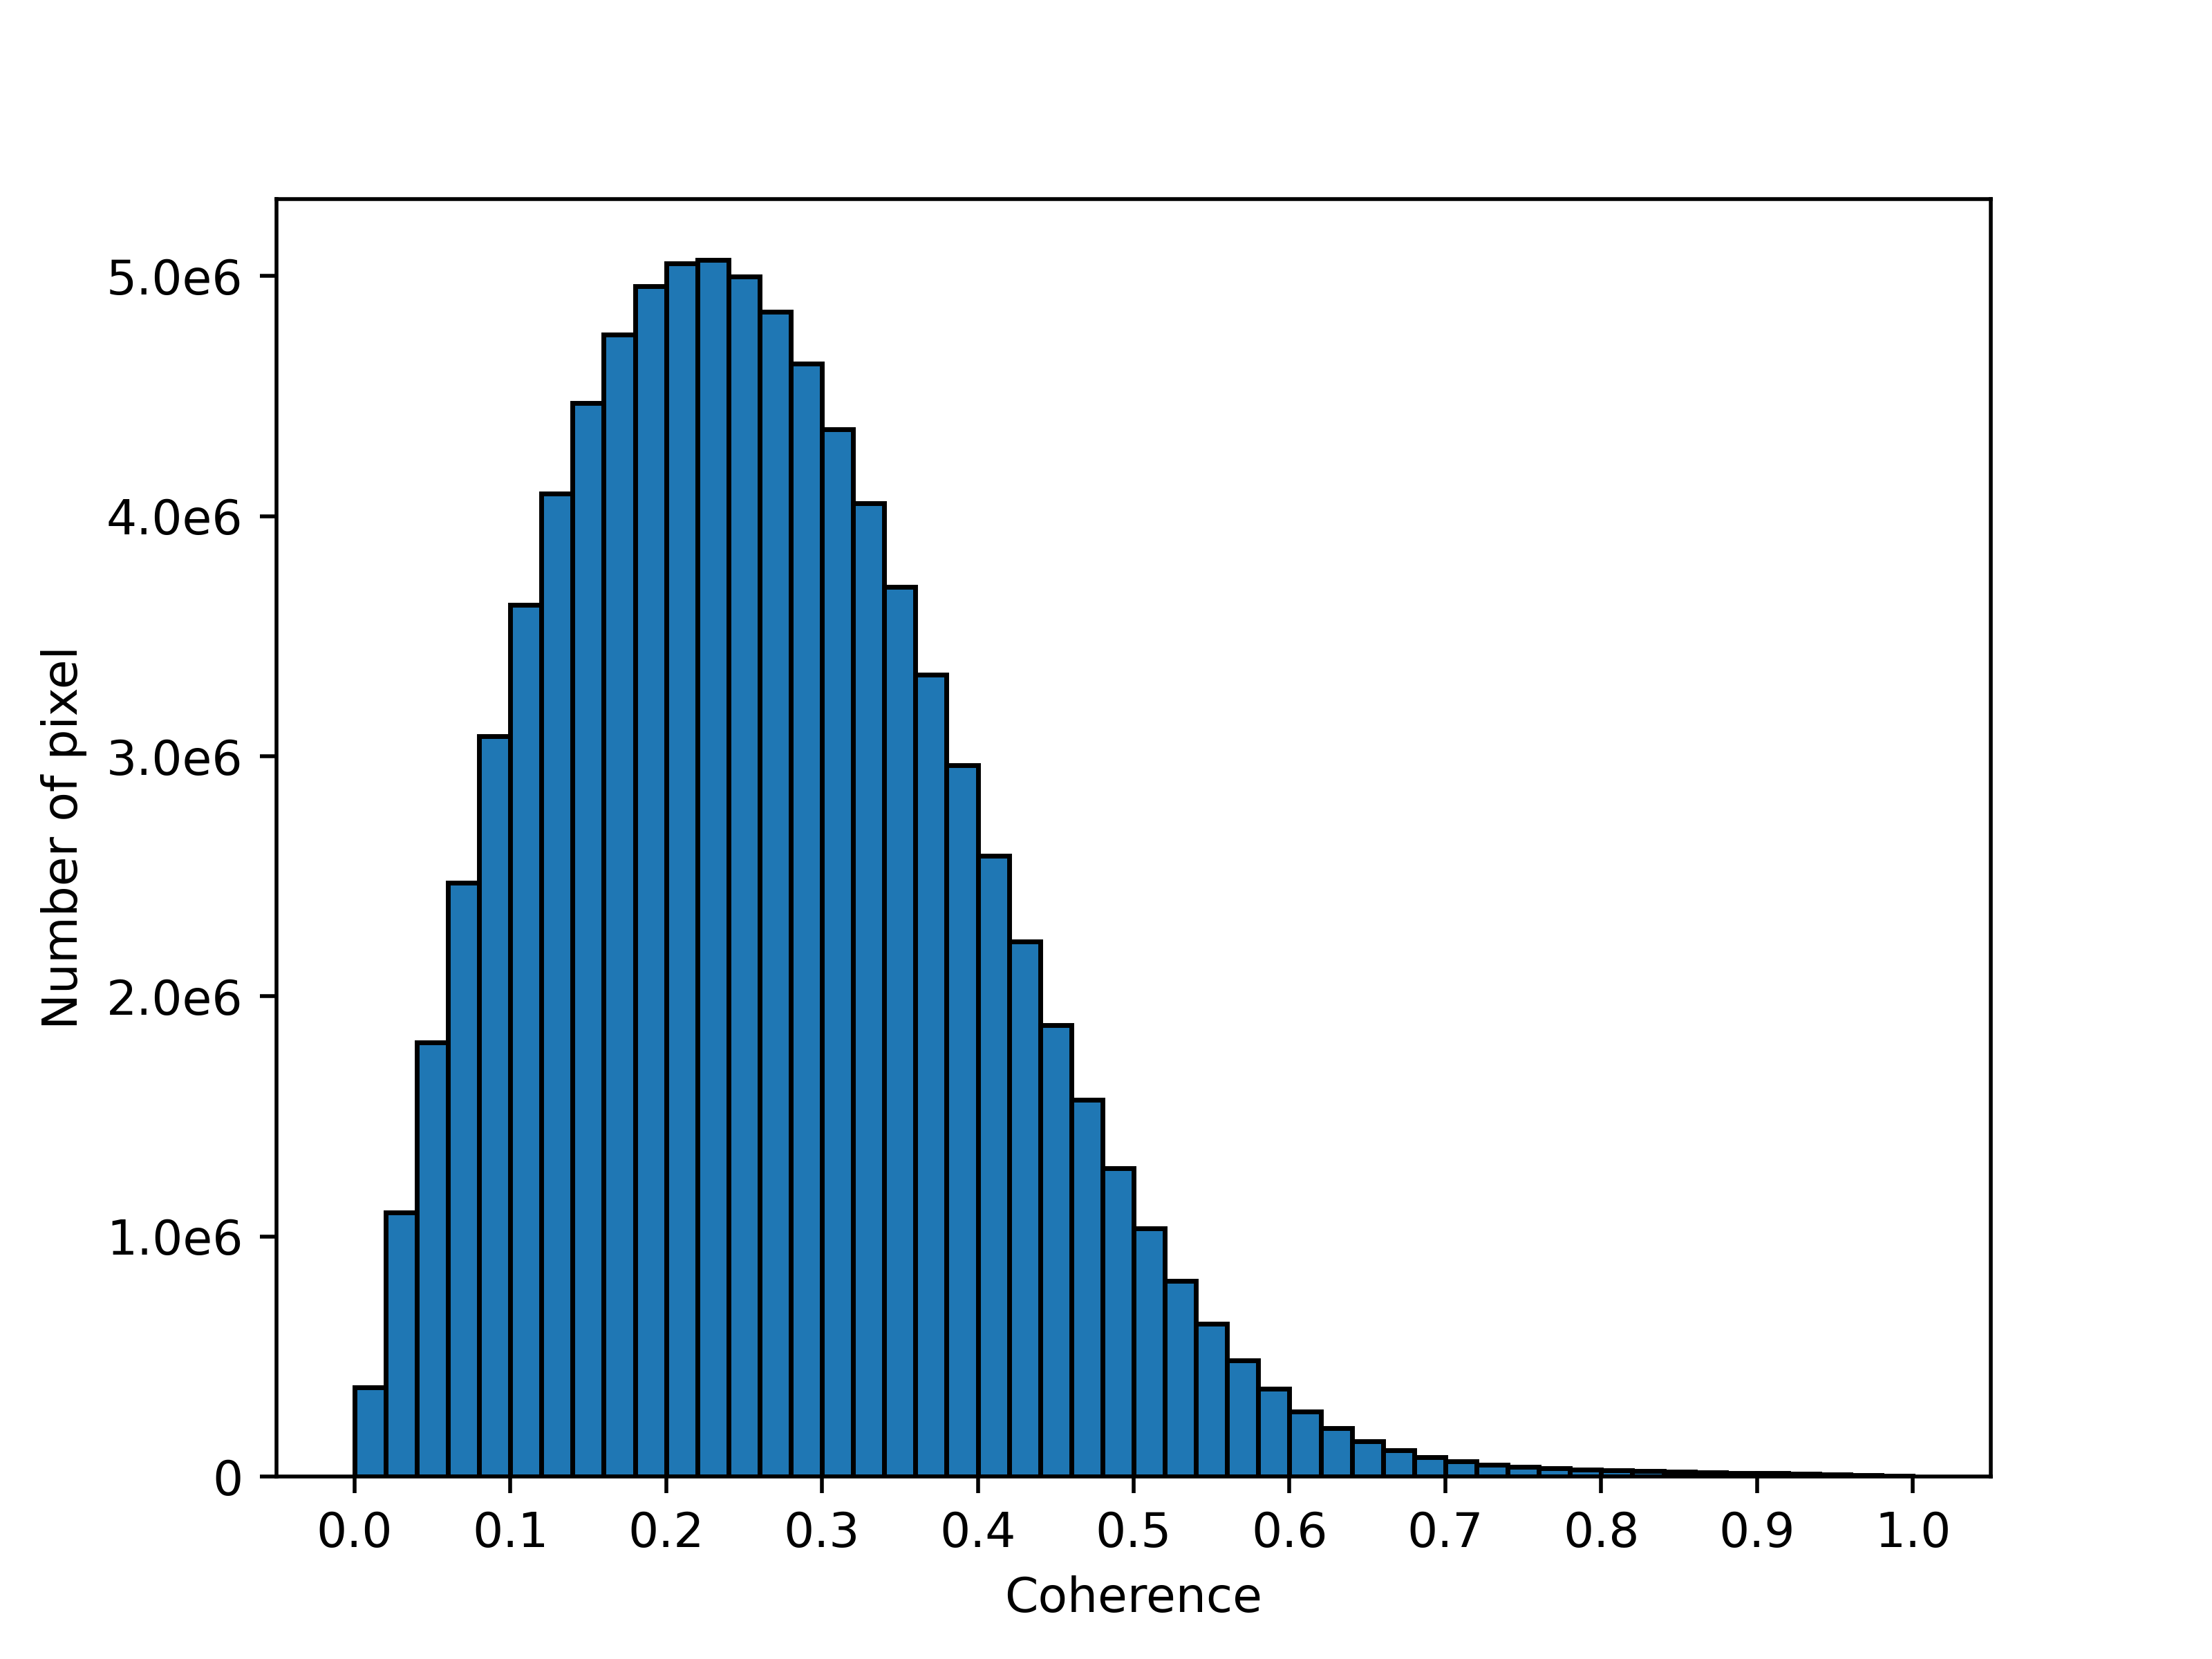
\includegraphics[width=\textwidth]{figure/The coherence/coh_Finland_asc_esd1_histogram_.png}
        \end{minipage}
        \caption{Finland ascending}
        \label{fig_6h}
    \end{subfigure}%
    \begin{subfigure}{0.5\textwidth}
        \centering
        \begin{minipage}{0.5\textwidth}
            \centering
            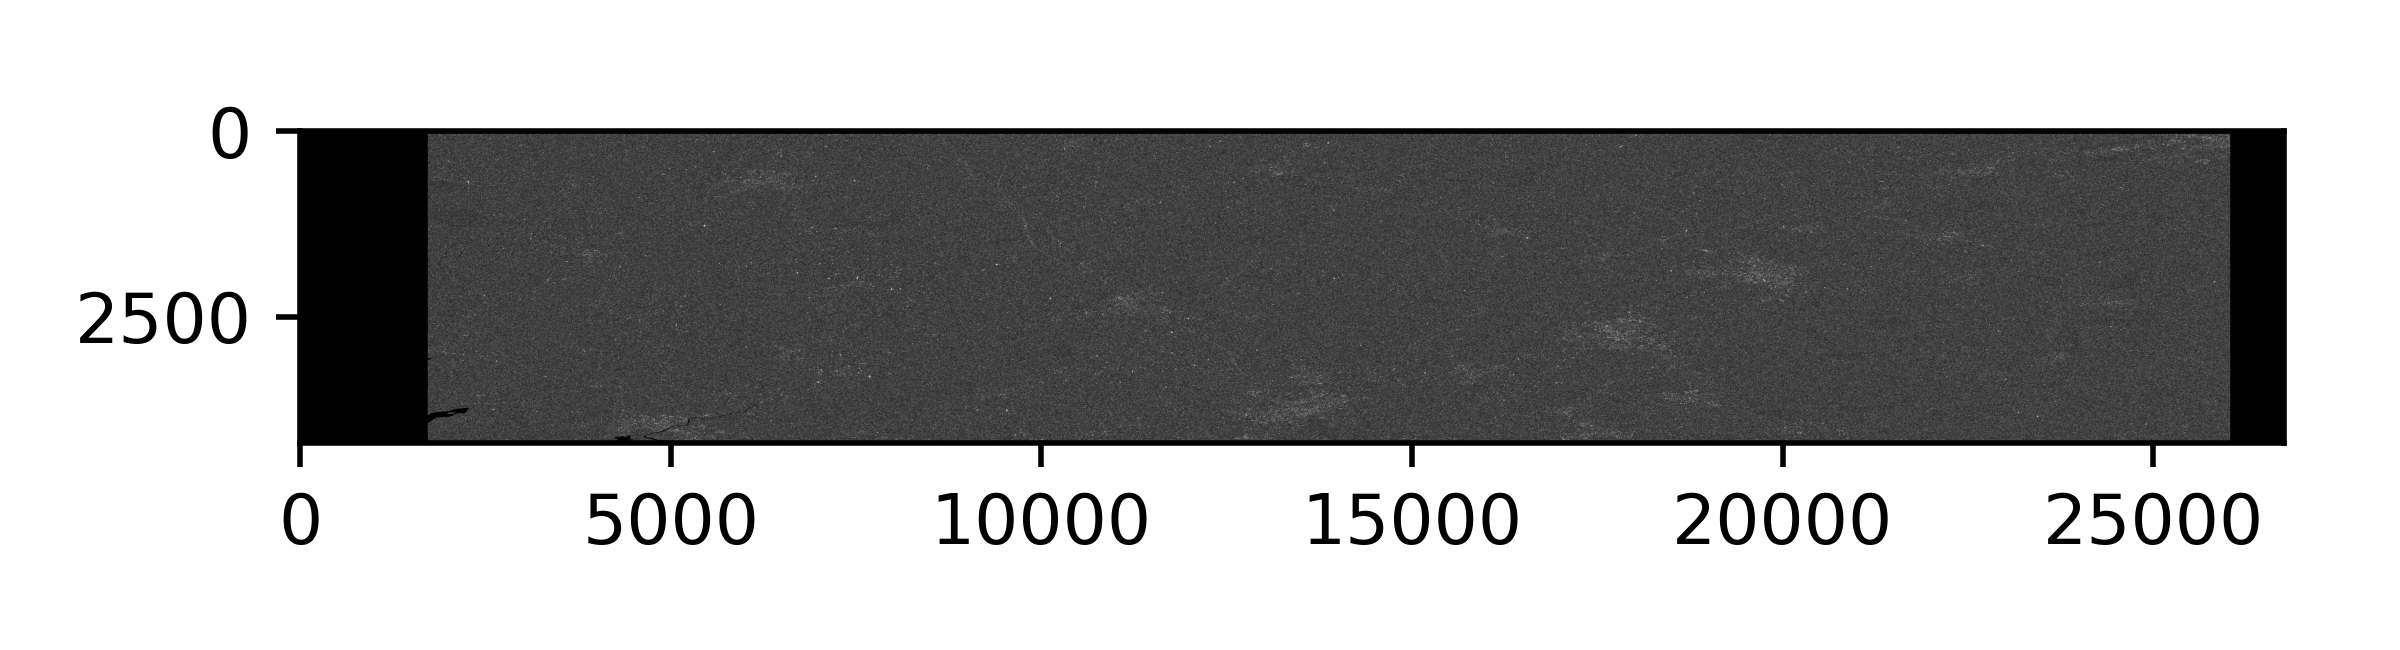
\includegraphics[width=\textwidth]{figure/The coherence/coh_Finland_des_esd1.png}
        \end{minipage}%
        \begin{minipage}{0.5\textwidth}
            \centering
            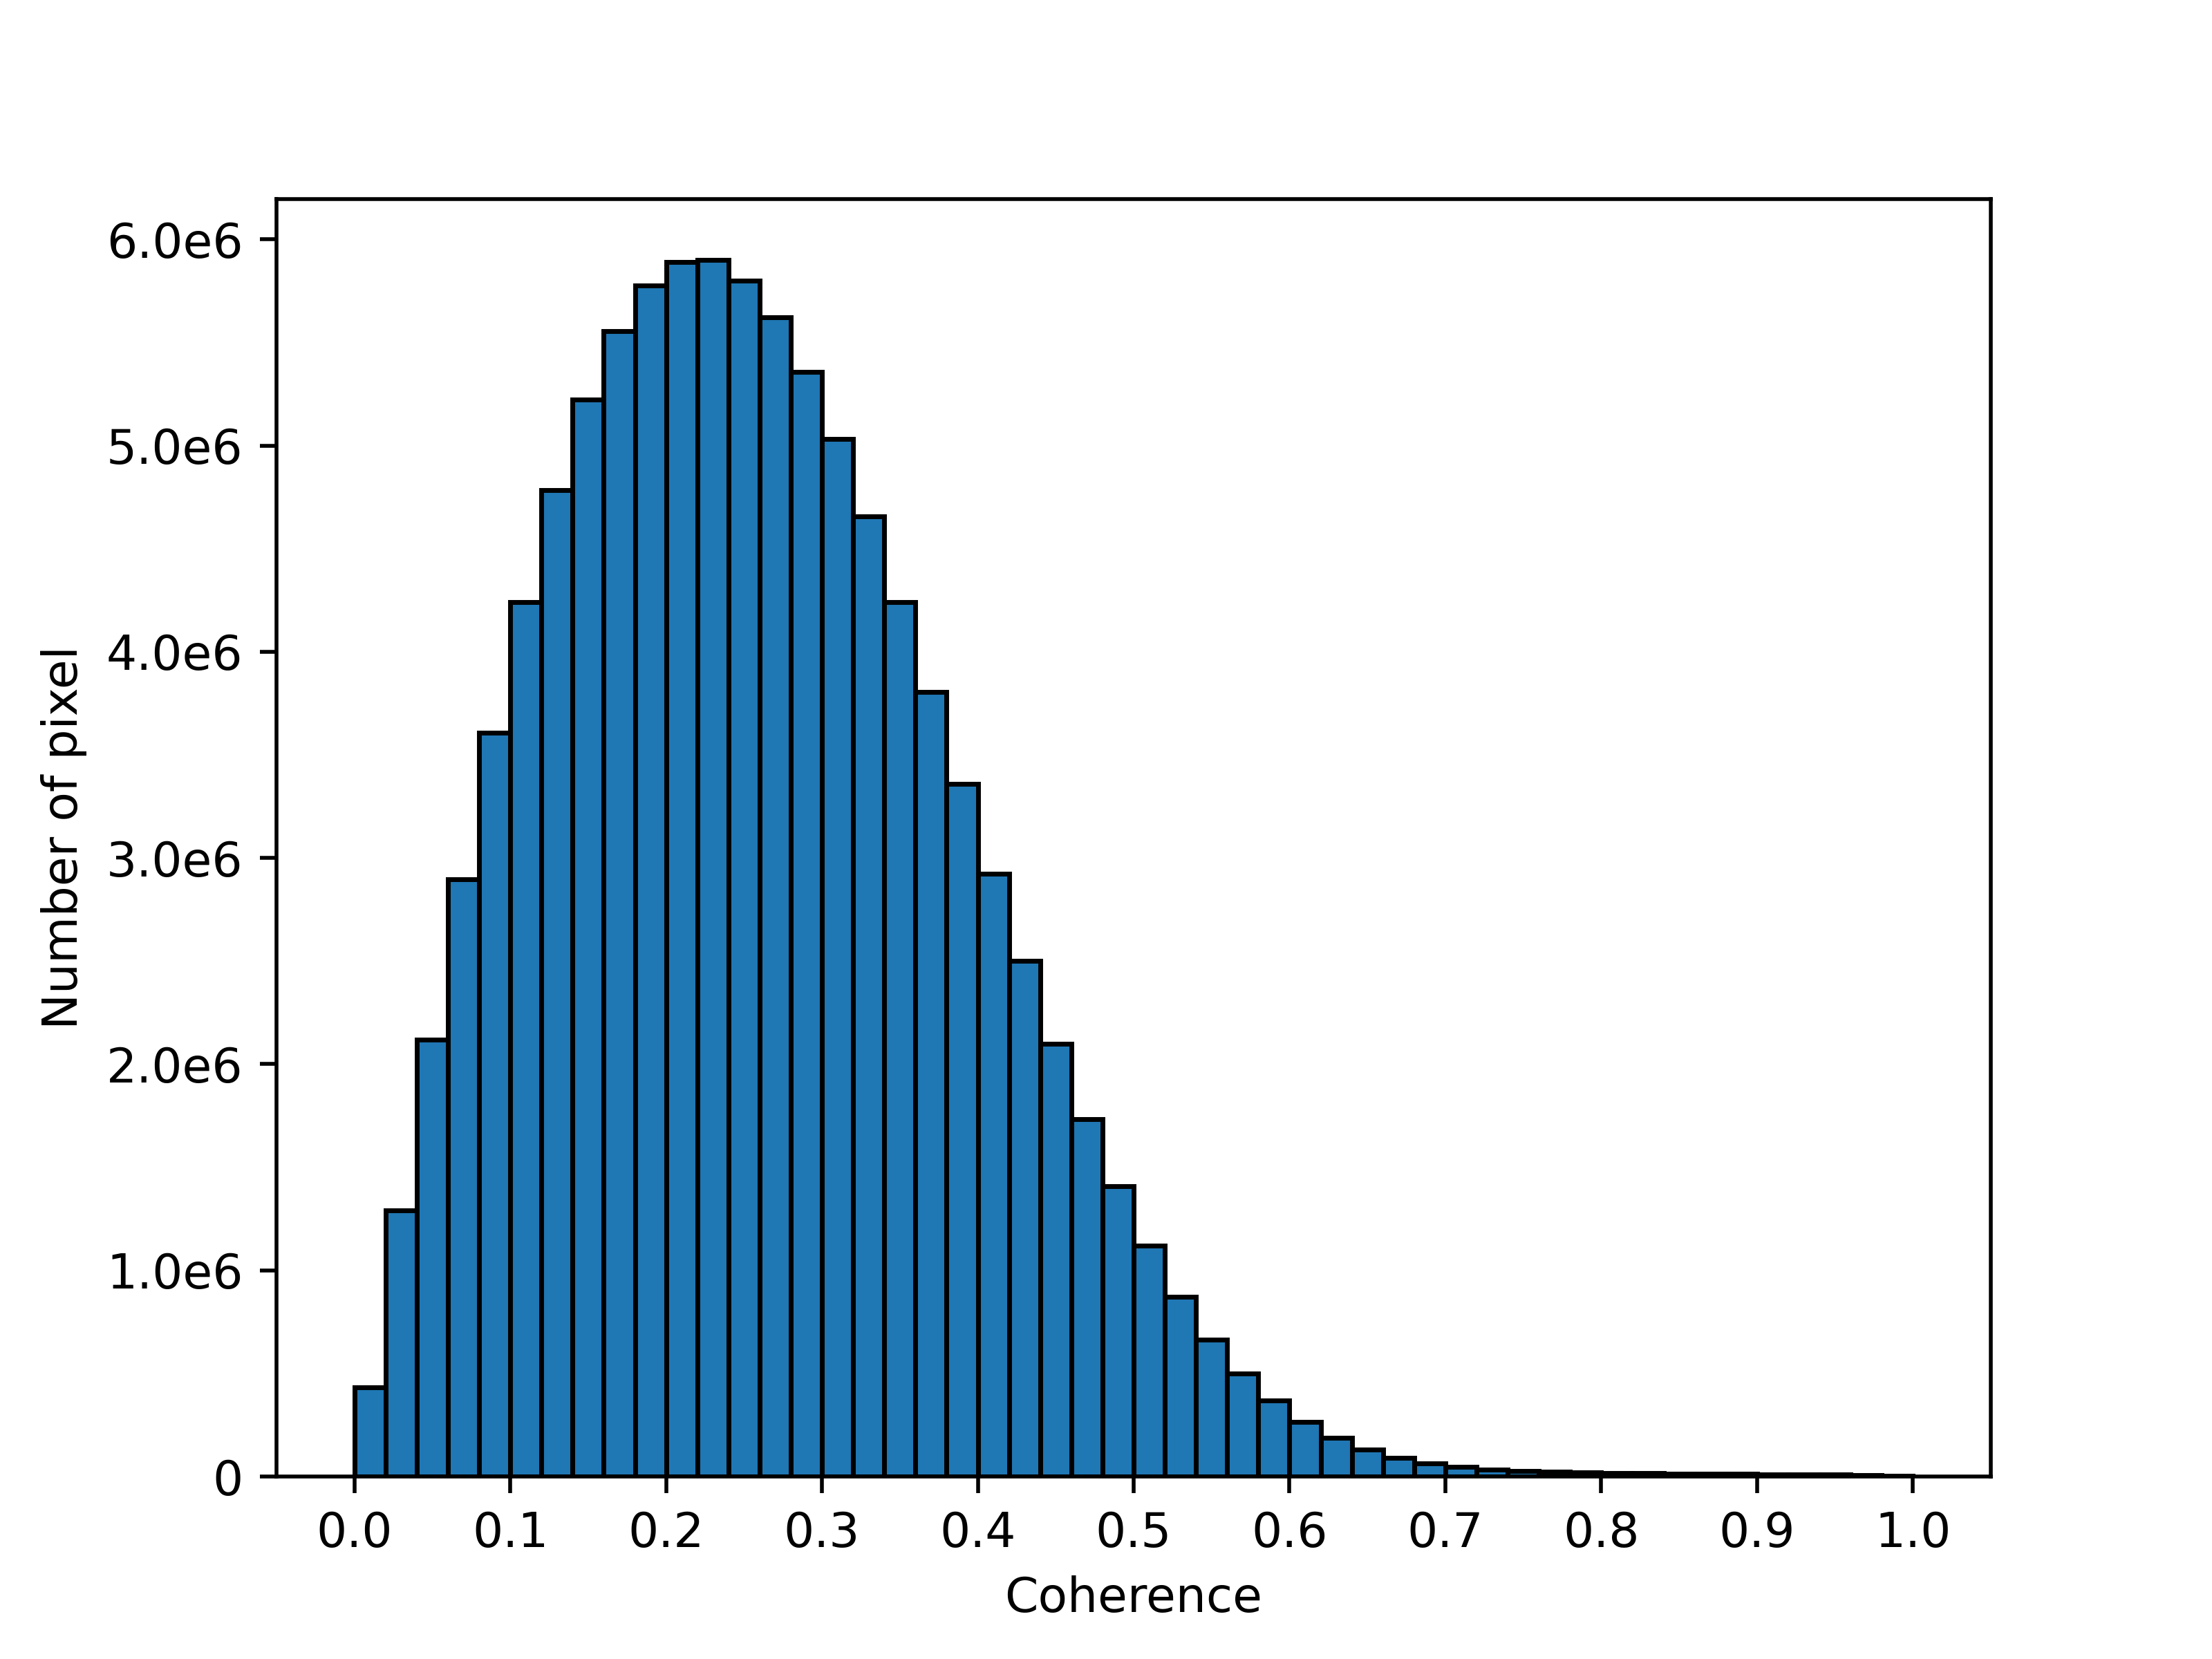
\includegraphics[width=\textwidth]{figure/The coherence/coh_Finland_des_esd1_histogram_.png}
        \end{minipage}
        \caption{Finland descending}
        \label{fig_6i}
    \end{subfigure}%
    \caption{The coherence and its distribution (Note: Taklamakan desert descending data is incomplete, and the results are selected from July 2022 to January 2023)}
    \label{fig_6}
\end{figure}

\subsection{Different Number of Bursts Experimental Result and Analysis}

When calculating the azimuth shift by ESD phase, the weight and the number of blocks are involved. Under different settings, the results may be different. Therefore, the interference experiment is carried out with the number of bursts as the independent variable, and the shifts calculated by different number of bursts in the same area are counted and compared. Different types of areas, the Taklamakan desert and Milan, were selected from January 2022 to December 2023, and the results are shown in \ref{table_5}. It can be seen from \ref{table_5} that different shifts are calculated by overlap area between different number of bursts in the same study area. The highest difference of mean is nearly 0.001 pixel, and the highest difference of standard deviation is nearly 0.001 pixel. In the face of the 0.001 pixel coregistration requirement required by TOPS, the above error magnitude cannot be ignored. Theoretically, the offset calculated by the ESD phase is a constant value, but in fact, the offset obtained by using different bursts calculations is different, and the magnitude of the difference between the offsets cannot be ignored. Therefore, it is necessary to pay attention to this when using ESD for fine coregistration, otherwise additional errors may be introduced. \par

\begin{table}[htbp]
\caption{The interference experiment result of different numbers of bursts}
\label{table_5}
\begin{minipage}[t]{\linewidth}
\centering
\begin{tabular*}{\linewidth}{@{\extracolsep{\fill}}>{\centering\arraybackslash}p{0.11\linewidth}>{\centering\arraybackslash}p{0.18\linewidth}*{10}{>{\centering\arraybackslash}p{0.042\linewidth}} }
\toprule
\multicolumn{2}{c}{\centering The serial number of the experiment} & 1 & 2 & 3 & 4 & 5 & 6 & 7 & 8 & 9 & 10 \\ % Table header row
\midrule
\multirow{2}{1\linewidth}{\centering Study area} & Taklamakan desert & $\bigcirc$ & $\bigcirc$ & $\bigcirc$ & $\bigcirc$ & $\bigcirc$ & $\bigcirc$ & $\bigcirc$ & $\bigcirc$ & $\bigcirc$ & $\bigcirc$ \\
 & Milan \\
\midrule
\multirow{2}{1\linewidth}{\centering Flight direction} & Ascending & $\bigcirc$ & $\bigcirc$ & $\bigcirc$ & $\bigcirc$ & $\bigcirc$ \\
 & Descending &  &  &  &  &  & $\bigcirc$ & $\bigcirc$ & $\bigcirc$ & $\bigcirc$ & $\bigcirc$ \\
\midrule
\multirow{5}{1\linewidth}{\centering Burst (start-end)} & 1-9 & $\bigcirc$ &  &  &  &  & $\bigcirc$ \\
 & 1-6 &  & $\bigcirc$ &  &  &  &  & $\bigcirc$ \\
 & 1-3 &  &  & $\bigcirc$ &  &  &  &  & $\bigcirc$ \\
 & 4-6 &  &  &  & $\bigcirc$ &  &  &  &  & $\bigcirc$ \\
 & 7-9 &  &  &  &  & $\bigcirc$ &  &  &  &  & $\bigcirc$ \\
\midrule
Shift & Mean value & -0.31 & -0.52 & -0.76 & -0.70 & -0.25 & -0.30 & -0.16 & -0.49 & -0.10 & 0.09 \\
($*10^{-3}$ pixel) & Standard deviation & 1.07 & 1.47 & 1.93 & 1.90 & 1.73 & 0.77 & 0.82 & 1.42 & 1.24 & 1.05 \\
\midrule
\multirow{2}{1\linewidth}{\centering Phase bias (radian)} & Mean value & -0.02 & -0.03 & -0.04 & -0.04 & -0.01 & -0.02 & -0.01 & -0.03 & -0.01 & 0.01 \\
 & Standard deviation & 0.06 & 0.08 & 0.11 & 0.11 & 0.10 & 0.04 & 0.05 & 0.08 & 0.07 & 0.06 \\
\bottomrule
\end{tabular*}
\end{minipage}

\vspace{0.1cm}

\begin{minipage}[t]{\linewidth}
\centering
\begin{tabular*}{\linewidth}{@{\extracolsep{\fill}}>{\centering\arraybackslash}p{0.11\linewidth}>{\centering\arraybackslash}p{0.18\linewidth}*{10}{>{\centering\arraybackslash}p{0.042\linewidth}} }
\toprule
\multicolumn{2}{c}{\centering The serial number of the experiment} & 1 & 2 & 3 & 4 & 5 & 6 & 7 & 8 & 9 & 10 \\ % Table header row
\midrule
\multirow{2}{1\linewidth}{\centering Study area} & Taklamakan desert \\
 & Milan & $\bigcirc$ & $\bigcirc$ & $\bigcirc$ & $\bigcirc$ & $\bigcirc$ & $\bigcirc$ & $\bigcirc$ & $\bigcirc$ & $\bigcirc$ & $\bigcirc$ \\
\midrule
\multirow{2}{1\linewidth}{\centering Flight direction} & Ascending & $\bigcirc$ & $\bigcirc$ & $\bigcirc$ & $\bigcirc$ & $\bigcirc$ \\
 & Descending &  &  &  &  &  & $\bigcirc$ & $\bigcirc$ & $\bigcirc$ & $\bigcirc$ & $\bigcirc$ \\
\midrule
\multirow{5}{1\linewidth}{\centering Burst (start-end)} & 1-9 & $\bigcirc$ &  &  &  &  & $\bigcirc$ \\
 & 1-6 &  & $\bigcirc$ &  &  &  &  & $\bigcirc$ \\
 & 1-3 &  &  & $\bigcirc$ &  &  &  &  & $\bigcirc$ \\
 & 4-6 &  &  &  & $\bigcirc$ &  &  &  &  & $\bigcirc$ \\
 & 7-9 &  &  &  &  & $\bigcirc$ &  &  &  &  & $\bigcirc$ \\
\midrule
Shift & Mean value & -1.44 & -1.44 & -2.08 & -1.02 & -0.64 & -4.09 & -3.32 & -3.28 & -4.20 & -4.89 \\
($*10^{-3}$ pixel) & Standard deviation & 1.71 & 1.78 & 2.01 & 1.80 & 2.10 & 1.65 & 1.69 & 1.61 & 1.89 & 1.88 \\
\midrule
\multirow{2}{1\linewidth}{\centering Phase bias (radian)} & Mean value & -0.08 & -0.08 & -0.12 & -0.06 & -0.04 & -0.27 & -0.22 & -0.22 & -0.28 & -0.33 \\
 & Standard deviation & 0.10 & 0.10 & 0.11 & 0.10 & 0.12 & 0.11 & 0.11 & 0.11 & 0.13 & 0.13 \\
\bottomrule
\end{tabular*}
\end{minipage}
\end{table}

In order to be more specific, the offsets of the Taklamakan Desert and Milan in different time ranges are selected as examples to illustrate. Using 9 bursts, there are 8 overlapping areas, each of which is divided into 10 blocks, so there are 8*10 offset results. Visualize the azimuth shift results, as shown in the \ref{fig_7}. Each pixel represents an offset, and the difference between the offsets is judged by the color depth. It can be seen from \ref{fig_7} that the results of different partitions are too different, which directly leads to the decrease of the accuracy of the calculation results. It is impossible to achieve accurate judgment only by image information such as weight, and more external factors need to be considered. \par

\begin{figure}
    \centering
    \begin{subfigure}{0.3\textwidth}
        \centering
        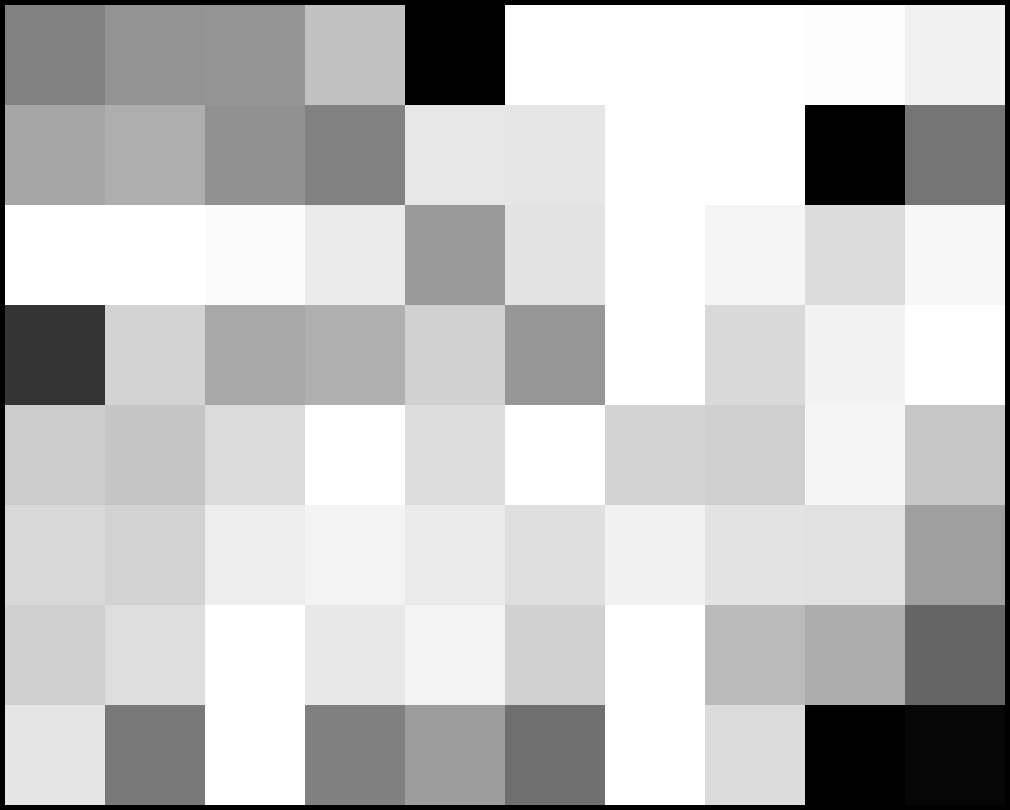
\includegraphics[width=\textwidth]{figure/The azimuth shift/shift_Milan_asc_20220626.png}
        \caption{2022.01 - 2022.06}
        \label{fig_7a}
    \end{subfigure}
    \begin{subfigure}{0.3\textwidth}
        \centering
        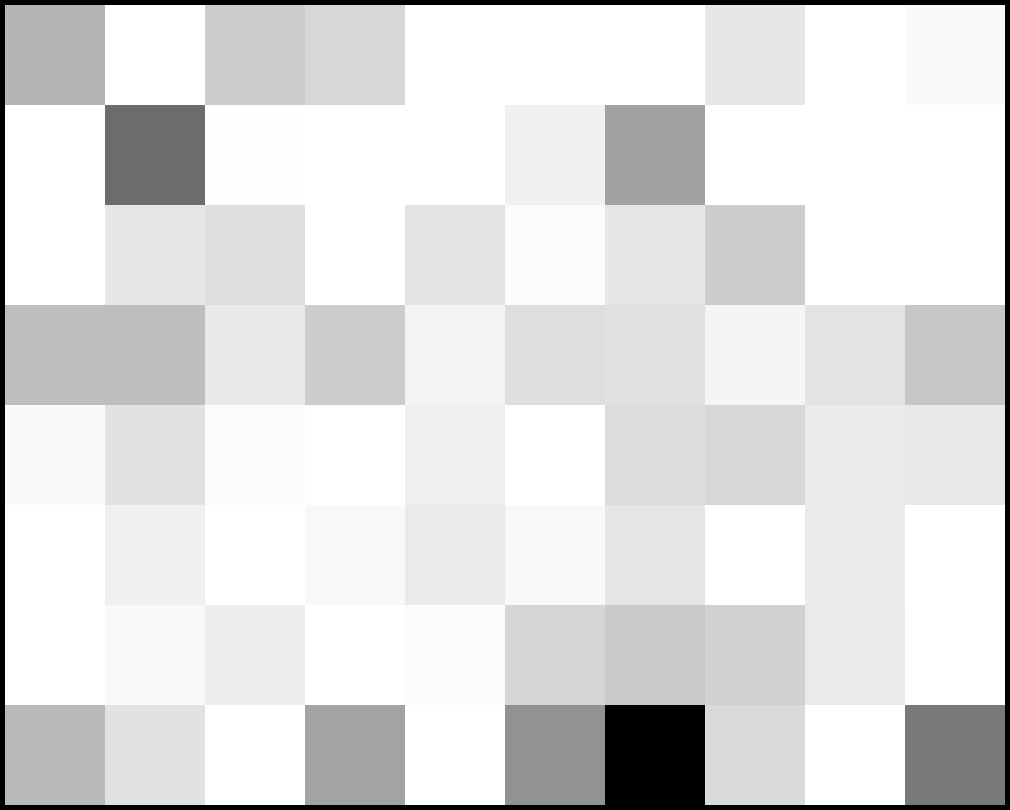
\includegraphics[width=\textwidth]{figure/The azimuth shift/shift_Milan_asc_20221223.png}
        \caption{2022.01 - 2022.12}
        \label{fig_7b}
    \end{subfigure}
    \begin{subfigure}{0.3\textwidth}
        \centering
        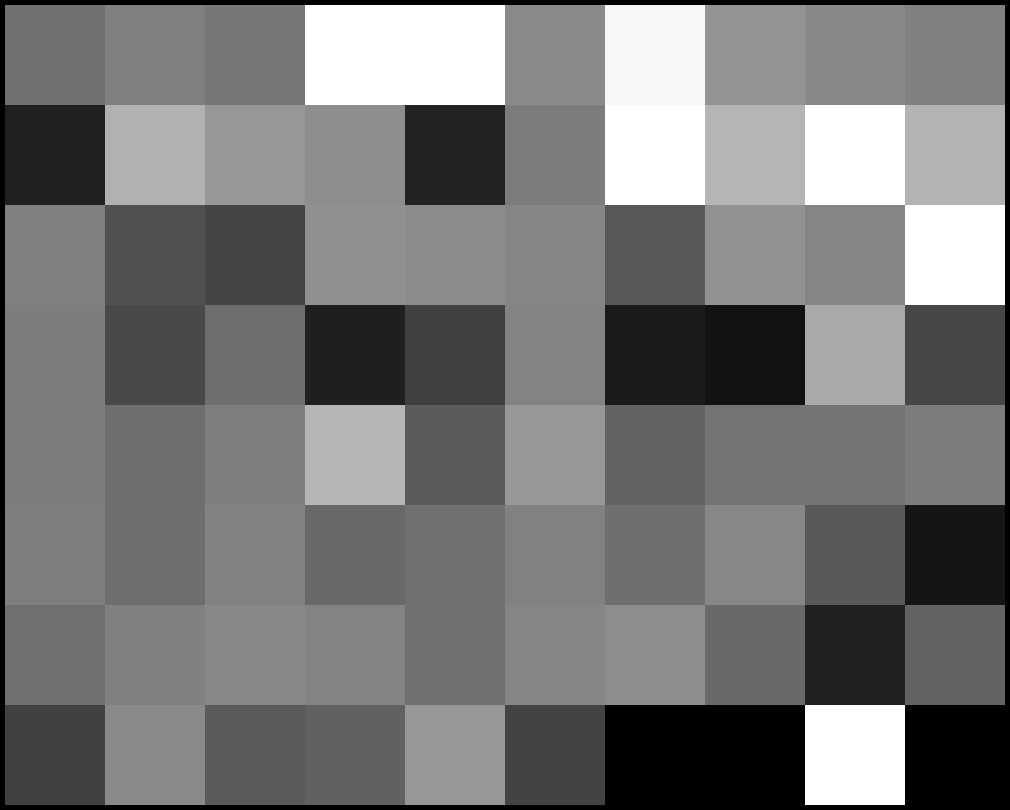
\includegraphics[width=\textwidth]{figure/The azimuth shift/shift_Milan_asc_20231230.png}
        \caption{2022.01 - 2023.12}
        \label{fig_7c}
    \end{subfigure}
    \hfill
    \begin{subfigure}{0.3\textwidth}
        \centering
        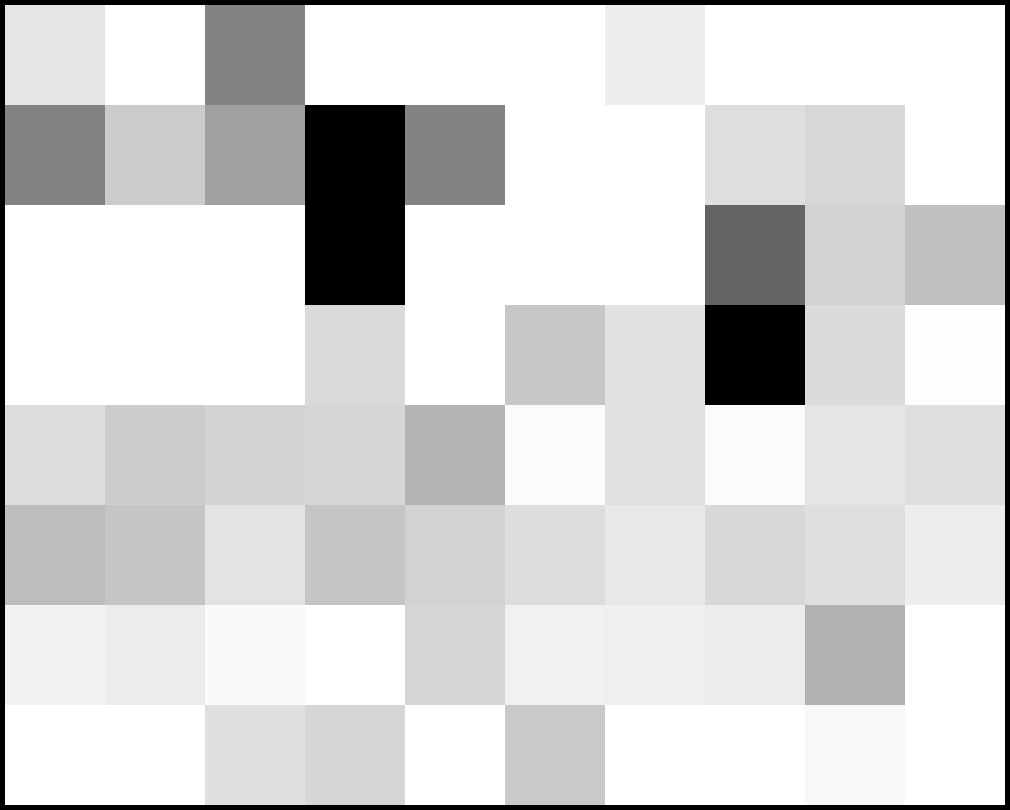
\includegraphics[width=\textwidth]{figure/The azimuth shift/shift_Milan_des_20220630.png}
        \caption{2022.01 - 2022.06}
        \label{fig_7d}
    \end{subfigure}
    \begin{subfigure}{0.3\textwidth}
        \centering
        \includegraphics[width=\textwidth]{figure/The azimuth shift/shift_Milan_des_20221227.png}
        \caption{2022.01 - 2022.12}
        \label{fig_7e}
    \end{subfigure}
    \begin{subfigure}{0.3\textwidth}
        \centering
        \includegraphics[width=\textwidth]{figure/The azimuth shift/shift_Milan_des_20231222.png}
        \caption{2022.01 - 2023.12}
        \label{fig_7f}
    \end{subfigure}
        \begin{subfigure}{0.3\textwidth}
        \centering
        \includegraphics[width=\textwidth]{figure/The azimuth shift/shift_TaklimakanDesert_asc_20220624.png}
        \caption{2022.01 - 2022.06}
        \label{fig_7j}
    \end{subfigure}
    \begin{subfigure}{0.3\textwidth}
        \centering
        \includegraphics[width=\textwidth]{figure/The azimuth shift/shift_TaklimakanDesert_asc_20221221.png}
        \caption{2022.01 - 2022.12}
        \label{fig_7h}
    \end{subfigure}
    \begin{subfigure}{0.3\textwidth}
        \centering
        \includegraphics[width=\textwidth]{figure/The azimuth shift/shift_TaklimakanDesert_asc_20231228.png}
        \caption{2022.01 - 2023.12}
        \label{fig_7ci}
    \end{subfigure}
    \hfill
    \begin{subfigure}{0.3\textwidth}
        \centering
        \includegraphics[width=\textwidth]{figure/The azimuth shift/shift_TaklimakanDesert_des_20221227.png}
        \caption{2022.07 - 2022.12}
        \label{fig_7g}
    \end{subfigure}
    \begin{subfigure}{0.3\textwidth}
        \centering
        \includegraphics[width=\textwidth]{figure/The azimuth shift/shift_TaklimakanDesert_des_20230625.png}
        \caption{2022.07 - 2023.06}
        \label{fig_7k}
    \end{subfigure}
    \begin{subfigure}{0.3\textwidth}
        \centering
        \includegraphics[width=\textwidth]{figure/The azimuth shift/colorbar.png}
        \caption*{}
    \end{subfigure}
    \caption{The azimuth shift (Note: a-c is the Milan ascending data, d-f is the Milan descending data, g-i is the Taklamakan desert ascending data, j-k is the Taklamakan desert descending data. The time intervals of half a year, one year and two years were selected respectively. Due to the incomplete data of the Taklamakan Desert, the results of the two-year interval are missing.)}
    \label{fig_7}
\end{figure}


\section{Discussion}

In this paper, the residual error after geometrical coregistration is judged by comparing the the azimuth shift difference and phase deviation. Importantly, in the experiment, we found two points of interest that need to be discussed in detail. \par

(1) The experimental results show that the residual error of geometrical coregistration does not decrease significantly from 2019 to 2020 regardless of the precise orbit data before and after adjustment. Taking the Milan ascending and descending experiments from May 2019 to September 2020 as an example, we calculate the difference between the azimuth shift of the slave images relative to the master image before and after the precise orbit configuration, as shown in the \ref{fig_8}. It can be seen from the \ref{fig_8} that the adjustment of the instantaneous position of the satellite in the azimuth direction is controlled within 4cm. Interference experiments show that the adjustment of this order of magnitude will not have a significant impact on geometrical coregistration. In addition, the same ARP and ANTEX configurations are not strictly used in the accuracy index during this period, and it is speculated that the accuracy of the control of the orbit itself may meet the requirements. Coregistration is a relative quantity between the master image and the slave image, while the orbit positioning accuracy is an absolute quantity. The \ref{eq_9} shows the mathematical relationship between the two, and most of the experimental results are within the accuracy range. \par

\begin{figure}
    \centering 
    \begin{subfigure}{0.5\textwidth}
        \centering
        \includegraphics[width=\textwidth]{figure/The azimuth shift of the slave images relative to the master image before and after the precise orbit configuration/asc.PNG}
        \caption{Milan ascending}
        \label{fig_8a}
    \end{subfigure}%
    \begin{subfigure}{0.5\textwidth}
        \centering
        \includegraphics[width=\textwidth]{figure/The azimuth shift of the slave images relative to the master image before and after the precise orbit configuration/des.png}
        \caption{Milan descending}
        \label{fig_8b}
    \end{subfigure}
    \caption{The azimuth shift of the slave images relative to the master image before and after the precise orbit configuration} 
    \label{fig_8}
\end{figure}

(2) After geometrical coregistration using precise orbit data with higher precision, the residual error is theoretically derived to be 0.0015 pixel by \ref{eq_9}, but the experimental results show that there is still an error of 0.002 to 0.003 pixel. The gap between theory and practice may be caused by factors from other sources. The premise of estimating geometrical coregistration error by ESD phase is to assume that the contribution of atmospheric phase screen (APS) and DEM error can be ignored \cite{Sentinel-1_precise_orbit_calibration_and_validation}. In some studies, it is suggested to use the stable overlap area between bursts to estimate the residual coregistration error \cite{Interferometry_with_TOPS:_coregistration_and_azimuth_shifts}. However, the actual ESD phase is not so ideal. In particular, under the requirement of TOPS high-precision coregistration, small phase errors cannot be ignored. On the one hand, the contribution of APS, such as water vapor delay and ionospheric disturbance, cannot be ignored. Previous studies have shown that the ionospheric phase screen can produce local azimuth delay in the image \cite{Interferometry_with_TOPS:_coregistration_and_azimuth_shifts}. On the other hand, any geophysical signal expressed in an almost constant manner in the monitoring scene cannot be separated from the geometrical error during coregistration \cite{Interferometry_with_TOPS:_coregistration_and_azimuth_shifts}. In addition to the above factors, it also includes the bistatic effects, frequency modulation rate miscoregistration, etc \cite{The_Extended_Timing_Annotation_Dataset_for_Sentinel-1—Product_Description_and_First_Evaluation_Results}. We call all the above factors as noise. In some studies, the spatio-temporal variability of the noise component in the data is described in detail by establishing a model of the spatio-temporal correlation between InSAR deformation monitoring \cite{Integrated_monitoring_of_subsidence_due_to_hydrocarbon_production:_consolidating_the_foundation, Radar_Interferometry_Data_Interpretation_and_Error_Analysis}. The essence of ESD phase is similar to InSAR deformation monitoring. For the S-1 TOPS IW data, the overlap area between the two bursts is about 14km in the azimuth direction. The standard deviation of the reference spatio-temporal variability is about 4mm, and the millimeter-scale deformation is calculated to the order of 0.001 to 0.01 pixel by \ref{eq_1}. The above errors can be classified as spatio-temporal variabi. \par


\section{Conclusion}
This paper aims at the coregistration method of S-1 TOPS, calculates the residual error of geometrical coregistration with the help of ESD, judges and evaluates the necessity of ESD assisted by higher precision orbit data, and studies the method to improve the coregistration efficiency. Considering a variety of factors, multiple types of data are selected for interference comparison experiments to draw universal conclusions. The conclusions include the following three points. (1) The accuracy of geometrical coregistration depends on the difference in the accuracy of the repeat orbit. The current precision orbit data released by the ESA has not had a significant impact on the accuracy of geometrical coregistration. (2) The error of geometrical coregistration mainly comes from the orbit error of the master image when registering multiple images of the repeat orbit. When the master image has no orbit error, the standard deviation of the coregistration error caused by the relative orbit error of the slave images relative to the master image is only 0.002 pixel. (3) Experiments show that the difference of ESD offset estimated by different bursts of the same track data is mostly more than 0.001 pixel, but in theory, the ESD offset of different bursts of the same track should be a constant value. Therefore, it is speculated that the coregistration error of 0.002 pixel may mainly come from the atmosphere, not the orbit error. The conclusion shows that if the constant value is used for correction of different bursts in the same orbit, it is possible to mistake the atmospheric error as the coregistration error correction. \par
ESD uses the phase inconsistency of the overlap area between bursts to perform constant offset to achieve coregistration, without considering the existence of many other interference sources in the phase, and is greatly affected by the coherence, which is ultimately reflected in the ESD mismatch accuracy. If the ESD method is used to simply perform a rigid change without considering this effect, it may bring additional coregistration errors to the results. Based on the above content, this paper gives corresponding suggestions. (1) For time series experiments, the influence of orbit error on phase is usually reduced with time series regression analysis. In the secondary coregistration process, the orbit error of the master image can be corrected by calculating the mean value of multiple interferograms, and the use of ESD may introduce additional errors. If you can accurately identify and correct phase artifacts from other sources, you can consider not correcting orbit errors \cite{InSAR_uncertainty_due_to_orbital_errors}. (2) For a single image experiment, the orbit error of the master image cannot be effectively estimated. When ESD must be used, this paper proposes a coregistration method based on phase without resampling, which can save 40\% of the calculation time. \par


% Numbered list
% Use the style of numbering in square brackets.
% If nothing is used, default style will be taken.
%\begin{enumerate}[a)]
%\item 
%\item 
%\item 
%\end{enumerate}  

% Unnumbered list
%\begin{itemize}
%\item 
%\item 
%\item 
%\end{itemize}  

% Description list
%\begin{description}
%\item[]
%\item[] 
%\item[] 
%\end{description}  

% % Figure
% \begin{figure}[<options>]
% 	\centering
% 		\includegraphics[<options>]{}
% 	  \caption{}\label{fig1}
% \end{figure}


% \begin{table}[<options>]
% \caption{}\label{tbl1}
% \begin{tabular*}{\tblwidth}{@{}LL@{}}
% \toprule
%   &  \\ % Table header row
% \midrule
%  & \\
%  & \\
%  & \\
%  & \\
% \bottomrule
% \end{tabular*}
% \end{table}

% Uncomment and use as the case may be
%\begin{theorem} 
%\end{theorem}

% Uncomment and use as the case may be
%\begin{lemma} 
%\end{lemma}

%% The Appendices part is started with the command \appendix;
%% appendix sections are then done as normal sections
%% \appendix


% To print the credit authorship contribution details
\printcredits

%% Loading bibliography style file
% \bibliographystyle{model1-num-names}
\bibliographystyle{cas-model2-names}

% Loading bibliography database
\bibliography{cas-refs}

% Biography
\bio{}
% Here goes the biography details.
\endbio

% \bio{pic1}
% % Here goes the biography details.
% \endbio

\end{document}

